%! Suppress = MissingImport
%! Suppress = TooLargeSection
%! Suppress = SentenceEndWithCapital
%! Suppress = LineBreak
%! Suppress = MissingLabel
%! Suppress = Unicode

\documentclass[main.tex]{subfiles}

\begin{document}

    \section{Metody dowodzenia poprawności pętli.}
    \section{Odwrotna Notacja Polska: definicja, własności, zalety i wady, algorytmy.}

    \subsection{Obliczanie wartości wyrażenia w ONP}
    \textbf{Przykład:}
    \[x ~ y ~ z ~ - ~ * ~ a ~ b ~ \text{\textasciicircum} ~ c ~ / ~ +\]

    Widok stosu:
    \begin{table}[H]
        \begin{tabular}{|p{2cm}|}
            \hline
            \textbf{x}\\
            \hline
            \hline
            \\
            \hline
            \\
            \hline
            x \\
            \hline
        \end{tabular}
        \begin{tabular}{|p{2cm}|}
            \hline
            \textbf{y}\\
            \hline
            \hline
            \\
            \hline
            y \\
            \hline
            x \\
            \hline
        \end{tabular}
        \begin{tabular}{|p{2cm}|}
            \hline
            \textbf{z}\\
            \hline
            \hline
            z \\
            \hline
            y \\
            \hline
            x \\
            \hline
        \end{tabular}
        \begin{tabular}{|p{2cm}|}
            \hline
            $\boldsymbol{-}$\\
            \hline
            \hline
            \\
            \hline
            y-z \\
            \hline
            x \\
            \hline
        \end{tabular}
        \begin{tabular}{|p{2cm}|}
            \hline
            $\boldsymbol{*}$\\
            \hline
            \hline
            \\
            \hline
            \\
            \hline
            x*(y-z)\\
            \hline
        \end{tabular}
    \end{table}
    \begin{table}[H]
        \begin{tabular}{|p{2cm}|}
            \hline
            \textbf{a}\\
            \hline
            \hline
            \\
            \hline
            a \\
            \hline
            x*(y-z)\\
            \hline
        \end{tabular}
        \begin{tabular}{|p{2cm}|}
            \hline
            \textbf{b}\\
            \hline
            \hline
            b \\
            \hline
            a \\
            \hline
            x*(y-z)\\
            \hline
        \end{tabular}
        \begin{tabular}{|p{2cm}|}
            \hline
            \textbf{\textasciicircum}\\
            \hline
            \hline
            \\
            \hline
            a \textasciicircum b\\
            \hline
            x*(y-z)\\
            \hline
        \end{tabular}
        \begin{tabular}{|p{2cm}|}
            \hline
            \textbf{c}\\
            \hline
            \hline
            c\\
            \hline
            a \textasciicircum b \\
            \hline
            x*(y-z)\\
            \hline
        \end{tabular}
        \begin{tabular}{|p{2cm}|}
            \hline
            $\boldsymbol{/}$\\
            \hline
            \hline
            \\
            \hline
            a \textasciicircum b /c\\
            \hline
            x*(y-z)\\
            \hline
        \end{tabular}
    \end{table}
    \begin{table}[H]
        \begin{tabular}{|p{3cm}|}
            \hline
            $\boldsymbol{+}$\\
            \hline
            \hline
            \\
            \hline
            \\
            \hline
            x*(y-z)+a \textasciicircum b/c\\
            \hline
        \end{tabular}
    \end{table}
    \textbf{Wyjście:}
    \[x*(y-z)+a\text{\textasciicircum}b/c\]

    \subsection{Zamiana wyrażenia infiksowego na ONP}
    \textbf{Przykład:}
    \[(a+b*c)\text{\textasciicircum}(x/y - z)\]

    \begin{table}[H]
        \begin{tabular}{|p{5cm}|p{5cm}|p{5cm}|}
            \hline
            \textbf{Wejście} & \textbf{Stos} & \textbf{Wyjście}\\
            \hline
            \hline
            $\boldsymbol{(}a+b*c)\text{\textasciicircum}(x/y - z)$ &&\\
            $\mathbf{a}+b*c)\text{\textasciicircum}(x/y - z)$ & $($ &\\
            $\boldsymbol{+}b*c)\text{\textasciicircum}(x/y - z)$ & $($ & $a$\\
            $\mathbf{b}*c)\text{\textasciicircum}(x/y - z)$ & $( ~ +$ & $a$\\
            $\boldsymbol{*}c)\text{\textasciicircum}(x/y - z)$  & $( ~ +$ & $a ~ b$\\
            $\mathbf{c})\text{\textasciicircum}(x/y - z)$  & $( ~ + ~ *$ & $a ~ b$\\
            $\boldsymbol{)}\text{\textasciicircum}(x/y - z)$  & $( ~ + ~ *$ & $a ~ b ~ c$\\
            $\text{\textbf{\textasciicircum}}(x/y - z)$  & & $a ~ b ~ c ~ * ~ +$\\
            $\boldsymbol{(}x/y - z)$  & \textasciicircum & $a ~ b ~ c ~ * ~ +$\\
            $\mathbf{x}/y - z)$  & \textasciicircum $($ & $a ~ b ~ c ~ * ~ +$\\
            $\boldsymbol{/}y - z)$  & \textasciicircum $($ & $a ~ b ~ c ~ * ~ + ~ x$\\
            $\mathbf{y} - z)$  & \textasciicircum $( ~ / $ & $a ~ b ~ c ~ * ~ + ~ x$\\
            $\boldsymbol{-} z)$  & \textasciicircum $( ~ / $ & $a ~ b ~ c ~ * ~ + ~ x ~ y$\\
            $\mathbf{z})$  & \textasciicircum $( ~ - $ & $a ~ b ~ c ~ * ~ + ~ x ~ y ~ /$\\
            $\boldsymbol{)}$  & \textasciicircum $( ~ - $ & $a ~ b ~ c ~ * ~ + ~ x ~ y ~ / ~ z$\\
            & \textasciicircum & $a ~ b ~ c ~ * ~ + ~ x ~ y ~ / ~ z -$\\
            & & $a ~ b ~ c ~ * ~ + ~ x ~ y ~ / ~ z - ~ $ \textasciicircum\\
            \hline
        \end{tabular}
    \end{table}
    \textbf{Wyjście:}
    \[a ~ b ~ c ~ * ~ + ~ x ~ y ~ / ~ z - ~ \text{\textasciicircum}\]

    \newpage

    \section{Modele obliczeń: maszyna Turinga.}

    Przykład: \textbf{Inkrementacja liczby binarnej}.\\

    \noindent Idea algorytmu:
    \begin{enumerate}
        \item Przechodź w prawo pomijając wszystkie znaki aż do znaku pustego.
        \item Przejdź w lewo drukując na znakach 1 znak 0 aż do oczytania znaku 0 lub znaku pustego.
        \item Wydrukuj znak 1 i zakończ.
    \end{enumerate}
    Przyjmujemy $b = \_$ (znak pusty).\\


    Zaczynamy od przechodzenia w prawo na koniec zapisu liczby:
    \begin{gather*}
        (A, 0) \mapsto (0, \rightarrow, A)\\
        (A, 1) \mapsto (1, \rightarrow, A)\\
    \end{gather*}

    Kiedy odczytamy znak pusty musimy zawrócić - tworzymy nowy stan (B), który będzie odpowiadał za przejście w lewo.
    \[ (A, \_) \mapsto (\_, \leftarrow, B) \]

    W stanie B przechodzimy wszystkie jedynki zastępując je zerami aż do natrafienia na 0 lub znak pusty:
    \begin{gather*}
        (B, 1) \mapsto (0, \leftarrow, B)\\
        (B, 0) \mapsto (1, \downarrow, Z)\\
        (B, \_) \mapsto (1, \downarrow, Z)\\
    \end{gather*}

    Gdzie Z jest stanem końcowym. Zatem nasza maszyna Turinga ma postać:
    \begin{gather*}
        MT = <Q, q_0, F, \tau, b, \delta>\\
        Q = \{A, B, Z\}\\
        q_0 = A\\
        F = \{Z\}\\
        \tau = \{ \_, 0, 1\}\\
        b = \_ \\
    \end{gather*}
    \begin{table}[H]
        \begin{center}
            \begin{tabular}{| p{1cm} || p{5cm} | p{5cm} | p{1cm} |}
                \hline
                $\boldsymbol{\delta}$ & \textbf{A} & \textbf{B} & \textbf{Z}\\
                \hline
                \hline
                \textbf{0} & $(0, \rightarrow, A)$ & $(1, \downarrow, Z)$ &\\
                \hline
                \textbf{1} & $(1, \rightarrow, A)$ & $(0, \leftarrow, B)$ &\\
                \hline
                $\boldsymbol{\_}$ & $(\_, \leftarrow, B)$ & $(1, \downarrow, Z)$ &\\
                \hline
            \end{tabular}
        \end{center}
    \end{table}

    \begin{center}
        \begin{tikzpicture}[scale=0.2]
            \tikzstyle{every node}+=[inner sep=0pt]
            \draw [black] (17,-19.8) circle (3);
            \draw (17,-19.8) node {$A$};
            \draw [black] (37,-36.3) circle (3);
            \draw (37,-36.3) node {$B$};
            \draw [black] (58.4,-25.6) circle (3);
            \draw (58.4,-25.6) node {$Z$};
            \draw [black] (58.4,-25.6) circle (2.4);
            \draw [black] (15.677,-17.12) arc (234:-54:2.25);
            \draw (17,-12.55) node [above] {$0,\mbox{ }0,\rightarrow$};
            \fill [black] (18.32,-17.12) -- (19.2,-16.77) -- (18.39,-16.18);
            \draw [black] (15.788,-22.531) arc (3.80557:-284.19443:2.25);
            \draw (11.26,-25.56) node [left] {$1,\mbox{ }1,\rightarrow$};
            \fill [black] (14.09,-20.5) -- (13.26,-20.05) -- (13.33,-21.05);
            \draw [black] (19.31,-21.71) -- (34.69,-34.39);
            \fill [black] (34.69,-34.39) -- (34.39,-33.5) -- (33.75,-34.27);
            \draw (23.88,-28.54) node [below] {$\_,\mbox{ }\_,\leftarrow$};
            \draw [black] (36.687,-39.272) arc (21.72436:-266.27564:2.25);
            \draw (30.29,-42.51) node [below] {$1,\mbox{ }0,\leftarrow$};
            \fill [black] (34.45,-37.86) -- (33.52,-37.69) -- (33.89,-38.62);
            \draw [black] (38.632,-33.785) arc (142.95131:90.1788:21.104);
            \fill [black] (55.41,-25.4) -- (54.61,-24.9) -- (54.61,-25.9);
            \draw (43.01,-27.11) node [above] {$0,\mbox{ }1,\downarrow$};
            \draw [black] (56.461,-27.887) arc (-43.47365:-83.39625:26.966);
            \fill [black] (56.46,-27.89) -- (55.55,-28.12) -- (56.27,-28.81);
            \draw (51.98,-33.97) node [below] {$\_,\mbox{ }1,\downarrow$};
            \draw [black] (6.7,-11.6) -- (14.65,-17.93);
            \fill [black] (14.65,-17.93) -- (14.34,-17.04) -- (13.72,-17.82);
        \end{tikzpicture}
    \end{center}

    \newpage

    \section{Modele obliczeń: automat skończony, automat ze stosem.}
    \subsection{Automat skończeniestanowy deterministyczny}
    \textbf{Zad 1.} \\

    \noindent Wykorzystując pochodne Brzozowskiego skonstruuj automat minimalny rozpoznający język $L = a(a+b)^{*}b(a+b)^{*}$ \\

    \noindent Wyznaczamy pochodne: \\
    $a^{-1}L = (a+b)^{*}b(a+b)^{*} = M$ \\
    $b^{-1}L = \emptyset$ \\
    $(aa)^{-1}L = M$ \\
    $(ab)^{-1}L = (a+b)^{*}b(a+b)^{*} + (a+b)^{*} = N$ \\
    $(aba)^{-1}L = N$ \\
    $(abb)^{-1}L = N$ \\

    \noindent Jak można zauważyć nie dostaniemy już innych pochodnych, więc nasz automat składa się z 4 stanów: L, $\emptyset$, M, N. \\
    Stan N jest stanem akceptującym, ponieważ został uzyskany przez odjęcie słowa należącego do języka L. L jest stanem początkowym. Przejściami w tym automacie są przejścia między pochodnymi pod wpływem kolejnych liter. \\

    \begin{center}
        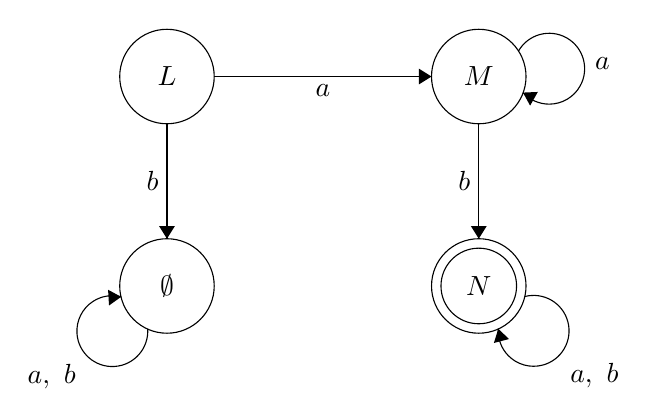
\begin{tikzpicture}[scale=0.2]
            \tikzstyle{every node}+=[inner sep=0pt]
            \draw [black] (17.3,-14.9) circle (3);
            \draw (17.3,-14.9) node {$L$};
            \draw [black] (17.3,-28.2) circle (3);
            \draw (17.3,-28.2) node {$\emptyset$};
            \draw [black] (37.1,-14.9) circle (3);
            \draw (37.1,-14.9) node {$M$};
            \draw [black] (37.1,-28.2) circle (3);
            \draw (37.1,-28.2) node {$N$};
            \draw [black] (37.1,-28.2) circle (2.4);
            \draw [black] (17.3,-17.9) -- (17.3,-25.2);
            \fill [black] (17.3,-25.2) -- (17.8,-24.4) -- (16.8,-24.4);
            \draw (16.8,-21.55) node [left] {$b$};
            \draw [black] (16.076,-30.926) arc (3.55967:-284.44033:2.25);
            \draw (11.54,-33.93) node [left] {$a,\mbox{ }b$};
            \fill [black] (14.39,-28.89) -- (13.56,-28.44) -- (13.62,-29.44);
            \draw [black] (20.3,-14.9) -- (34.1,-14.9);
            \fill [black] (34.1,-14.9) -- (33.3,-14.4) -- (33.3,-15.4);
            \draw (27.2,-15.4) node [below] {$a$};
            \draw [black] (39.617,-13.29) arc (150.34019:-137.65981:2.25);
            \draw (44.46,-14.05) node [right] {$a$};
            \fill [black] (39.91,-15.92) -- (40.36,-16.75) -- (40.85,-15.88);
            \draw [black] (37.1,-17.9) -- (37.1,-25.2);
            \fill [black] (37.1,-25.2) -- (37.6,-24.4) -- (36.6,-24.4);
            \draw (36.6,-21.55) node [left] {$b$};
            \draw [black] (40.011,-28.873) arc (104.71059:-183.28941:2.25);
            \draw (42.88,-33.91) node [right] {$a,\mbox{ }b$};
            \fill [black] (38.34,-30.92) -- (38.06,-31.82) -- (39.02,-31.57);
        \end{tikzpicture}
    \end{center}

    \noindent \textbf{Zad 2.}

    \noindent Dany jest automat $al{A}$ = (S, f) nad alfabetem A = \{a, b\}, tak że $S = \{s_{0}, s_{1}, s_{2}\}$.
    \begin{table}[H]
        \centering
        \begin{tabular}{|c|l|l|l|}
            \hline
            f & $s_{0}$ & $s_{1}$ & $s_{2}$ \\ \hline
            a & $s_{1}$ & $s_{2}$ & $s_{2}$ \\ \hline
            b & $s_{0}$ & $s_{0}$ & $s_{2}$ \\ \hline
        \end{tabular}
    \end{table}
    \noindent Określ dla tego automatu jego reprezentację oraz monoid przejść.

    \begin{center}
        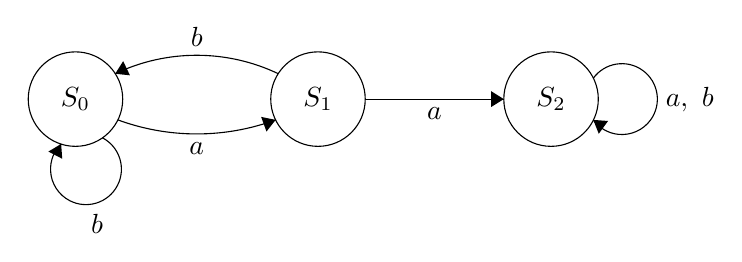
\begin{tikzpicture}[scale=0.2]
            \tikzstyle{every node}+=[inner sep=0pt]
            \draw [black] (17.6,-22.6) circle (3);
            \draw (17.6,-22.6) node {$S_0$};
            \draw [black] (33,-22.6) circle (3);
            \draw (33,-22.6) node {$S_1$};
            \draw [black] (47.8,-22.6) circle (3);
            \draw (47.8,-22.6) node {$S_2$};
            \draw [black] (30.311,-23.919) arc (-69.79109:-110.20891:14.507);
            \fill [black] (30.31,-23.92) -- (29.39,-23.73) -- (29.73,-24.66);
            \draw (25.3,-25.31) node [below] {$a$};
            \draw [black] (36,-22.6) -- (44.8,-22.6);
            \fill [black] (44.8,-22.6) -- (44,-22.1) -- (44,-23.1);
            \draw (40.4,-23.1) node [below] {$a$};
            \draw [black] (50.48,-21.277) arc (144:-144:2.25);
            \draw (55.05,-22.6) node [right] {$a,\mbox{ }b$};
            \fill [black] (50.48,-23.92) -- (50.83,-24.8) -- (51.42,-23.99);
            \draw [black] (19.305,-25.054) arc (62.53077:-225.46923:2.25);
            \draw (18.97,-29.87) node [below] {$b$};
            \fill [black] (16.69,-25.45) -- (15.88,-25.93) -- (16.76,-26.39);
            \draw [black] (20.12,-20.987) arc (115.48516:64.51484:12.038);
            \fill [black] (20.12,-20.99) -- (21.06,-21.09) -- (20.63,-20.19);
            \draw (25.3,-19.32) node [above] {$b$};
        \end{tikzpicture}
    \end{center}

    \noindent Określamy reprezentację uzupełniając tabelkę wpisując po lewej stronie kolejne słowa, a w kolejnych kolumnach stan w jakim się znajdziemy po przejściu pod wpływem tego słowa zaczynając od stanu z wiersza u samej góry: \\

    \begin{table}[H]
        \centering
        \begin{tabular}{|c|l|l|l|}
            \hline
            & $s_{0}$ & $s_{1}$ & $s_{2}$ \\ \hline
            1 & $s_{0}$ & $s_{1}$ & $s_{2}$ \\ \hline
            a & $s_{1}$ & $s_{2}$ & $s_{2}$ \\ \hline
            b & $s_{0}$ & $s_{0}$ & $s_{2}$ \\ \hline
            $a^2$  & $s_{2}$ & $s_{2}$ & $s_{2}$ \\ \hline
            ab & $s_{0}$ & $s_{2}$ & $s_{2}$ \\ \hline
            ba & $s_{1}$ & $s_{1}$ & $s_{2}$ \\ \hline
        \end{tabular}
    \end{table}

    \noindent Powyższa tabelka przedstawia już wszystkie możliwe kombinacje stanów do uzyskania dla tego automatu (kolejne słowa dawałyby stan, który już jest w tabelce dla innego słowa) i jest ona reprezentacją naszego automatu. \\

    \noindent Dodatkowo możemy podczas uzupełniania tabelki zauważyć m.in. że: \\
    $b^2 = b$ \\
    $a^3 = a^2$ \\
    $a^{2}b = a^2$ \\
    co może nam ułatwić jej uzupełnianie. \\

    \noindent Monoidem przejść nazywamy zbiór tych słów, które udało nam się uzyskać w naszej tabelce: \\
    $\mathcal{M(A)}$ = \{1, a, b, $a^2$, ab, ba, $b^2$\} = $\tau \mathcal{A}(A^{*})$

    \subsection{Automat ze stosem}
    Dany jest automat ze stosem gdzie: \\
    $A_{S} = \{z_{0}, a\}$ $A = \{a, b, c\}$, $Q = \{q_{0}, q_{1}, q_{2}\}$ \\
    $P = \{z_{0}q_{0}a \rightarrow aq_{0}, aq_{0}a \rightarrow a^2 q_{0}, aq_{0}b \rightarrow a^2 q_{1}, aq_{1}b \rightarrow a^2 q_{1}, aq_{1}c \rightarrow 1q_{2}, aq_{2}c \rightarrow 1q_{2}\}$ \\

    \noindent Narysuj graf automatu i określ język akceptowany przez pusty stos: \\

    \begin{center}
        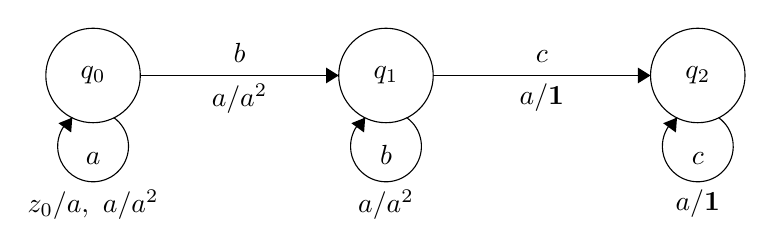
\begin{tikzpicture}[scale=0.2]
            \tikzstyle{every node}+=[inner sep=0pt]
            \draw [black] (15,-24.8) circle (3);
            \draw (15,-24.8) node {$q_0$};
            \draw [black] (33.6,-24.8) circle (3);
            \draw (33.6,-24.8) node {$q_1$};
            \draw [black] (53.4,-24.8) circle (3);
            \draw (53.4,-24.8) node {$q_2$};
            \draw [black] (16.323,-27.48) arc (54:-234:2.25);
            \draw (15,-30.5) node [above] {$a$};
            \draw (15,-32.05) node [below] {$z_0/a,\mbox{ }a/a^2$};
            \fill [black] (13.68,-27.48) -- (12.8,-27.83) -- (13.61,-28.42);
            \draw [black] (18,-24.8) -- (30.6,-24.8);
            \fill [black] (30.6,-24.8) -- (29.8,-24.3) -- (29.8,-25.3);
            \draw (24.3,-24) node [above] {$b$};
            \draw (24.3,-25.3) node [below] {$a/a^2$};
            \draw [black] (34.923,-27.48) arc (54:-234:2.25);
            \draw (33.6,-30.5) node [above] {$b$};
            \draw (33.6,-32.05) node [below] {$a/a^2$};
            \fill [black] (32.28,-27.48) -- (31.4,-27.83) -- (32.21,-28.42);
            \draw [black] (54.723,-27.48) arc (54:-234:2.25);
            \draw (53.4,-30.5) node [above] {$c$};
            \draw (53.4,-32.05) node [below] {$a/\mathbf{1}$};
            \fill [black] (52.08,-27.48) -- (51.2,-27.83) -- (52.01,-28.42);
            \draw [black] (36.6,-24.8) -- (50.4,-24.8);
            \fill [black] (50.4,-24.8) -- (49.6,-24.3) -- (49.6,-25.3);
            \draw (43.5,-24) node [above] {$c$};
            \draw (43.5,-25.3) node [below] {$a/\mathbf{1}$};
        \end{tikzpicture}
    \end{center}

    \noindent Językiem akceptowanym przez ten automat jest język $a^{N}b^{M}c^{N+M}$, gdzie N, M $>$ 0.


    \newpage

    \section{Złożoność obliczeniowa - definicja notacji: $O, \Omega, \Theta$.}

    \newpage

    \section{Złożoność obliczeniowa - pesymistyczna i średnia.}

    \begin{exercise}
        Oblicz pesymistyczną i średnią złożoność obliczeniową algorytmu sortowania przez wstawianie.
    \end{exercise}

    \textbf{Złożoność pesymistyczna}

    Przypadek pesymistyczny polega na otrzymaniu na wejściu odwrotnie posortowanej tablicy.
    Wówczas każdy element (oprócz pierwszego) z zostanie porównany
    i zamieniony ze wszystkimi elementami uprzednio posortowanego fragmentu tablicy.
    Obliczmy złożoność zakładając, że zamiana elementów zajmuje czas równy stałej $c$.

    \begin{gather*}
        W(c) = \sum_{i = 2}^n ic\\
        W(c) = \frac{n^2 + n - 2}{2}c\\
        W(c) = \theta(n^2)\\
    \end{gather*}

    \textbf{Złożoność średnia}

    Zauważmy, że ilość zamian elementów jest zależna od liczby inwersji w tablicy wejściowej. Aby obliczyć średnią złożoność algorytmu musimy obliczyć średnią liczbę inwersji.\\

    Niech $X_{ij}$ będzie zmienną losową oznaczającą, czy w tablicy wejściowej $A[i]$ jest w inwersji z $A[j]$.
    Ilość par $i,j$ jest równa $\frac{n(n-1)}{2}.$

    \[A(n) = E\left(\sum X_{ij}\right) = \sum E(X_i j) = \frac{1}{2} \cdot \frac{n(n - 1)}{2} = \frac{n(n - 1)}{4}\]

    \begin{exercise}
        Oblicz średnią złożoność obliczeniową algorytmu quicksort.
    \end{exercise}

    Zakładamy, że tablica wejściowa nie posiada duplikatów, zaś operacją dominującą jest porównywanie.
    Przy każdym wyborze elementu rozdzielającego ilość elementów od niego mniejsza jest zmienną losową od 0 do $n - 1$ o rozkładzie jednostajnym.
    Zatem po podziale otrzymujemy dwie tablice: o długości $i$ oraz o długości $n - i - 1$ gdzie $i$ jest zmienną losową o rozkładzie jednostajnym od 0 do $n - 1$.
    Zatem zakładając, że ilość porównań przy każdym podziale wynosi $n - 1$, średnia ilość porównań dla wszystkich permutacji otrzymanej tablicy jest równa:
    \begin{align*}
        &A(n) = n - 1 + \frac{1}{n}\sum_{i = 0}^{n - 1}(A(i) + A(n - i - 1)) =
        n - 1 + \frac{2}{n}\sum_{i = 0}^{n - 1}A(i)\\
        &nA(n) = n(n - 1) + 2 \sum_{i = 0}^{n - 1}A(i)\\
        &nA(n) - (n - 1)A(n-1) = n(n - 1) - (n - 1)(n - 2) + 2\sum_{i = 0}^{n - 1}A(i) - 2\sum_{i = 0}^{n - 2}A(i) =\\
        &= 2(n - 1) + 2A(n - 1)\\
        &\\
        &nA(n) = (n + 1)A(n - 1) + 2n - 2\\
        &\\
        &A(n) = \frac{(n + 1)A(n - 1)}{n} + 2 - \frac{2}{n}\\
        &\frac{A(n)}{n + 1} = \frac{A(n - 1)}{n} + \frac{2}{n + 1} - \frac{2}{n(n + 1)}
        = \frac{A(n - 2)}{n - 1} + \frac{2}{n} - \frac{2}{(n - 1)n} - \frac{2}{n(n + 1)} + \frac{2}{n + 1} =\\
        &= \cdots = \frac{A(1)}{2} + \sum_{i = 2}^n \frac{2}{i + 1} - \sum_{i = 2}^n \frac{2}{i(i + 1)} =
        2\sum_{i = 1}^{n - 1} \frac{1}{i} - \frac{n - 1}{n + 1}\\
        &\\
        &\sum_{i = 1}^{n - 1} \frac{1}{i} \approx \int_1^{n - 1}\frac{dx}{x} = ln(n - 1)\\
        &\\
        &A(n) = 2(n + 1)\;ln(n - 1) - n + 1 = 2n\;ln(n - 1) + 2ln(n - 1) - n + 1 \leq\\
        &\leq 2\;ln(n) \approx 1.39 n \; log_2 n = \theta(n\;ln(n))\\
    \end{align*}

    \newpage


    \section{Metoda "dziel i zwyciężaj": zalety i wady.}

    \subsection{Binary search}

    Problem: dla zadanej posortowanej tablicy $A$ o długości $n$, znajdź indeks elementu
    równego $x$ lub zwróć -1 w przypadku braku $x$ w tablicy $A$.
    \[\]
    Działamy na (zmniejszającym się) przedziale tablicy $A$. Indeks początka przedziału:
    $l = 0$, indeks końca przedziału: $r = n - 1$.

    \begin{enumerate}
        \item \textbf{Dziel}

        Porównaj element $A[s]$ ($s = \frac{l+ r}{2}$) z $x$.

        \begin{itemize}
            \item $A[s] = x$

            Zwróć $s$.

            \item $A[s] > x$

            Powtórz dla $A[l : s - 1]$, tzn $l = l, r = s - 1$

            \item $A[s] < x$

            Powtórz rekurencyjnie dla $A[s + 1 : n - 1]$, tzn $l = s + 1, r = r$
        \end{itemize}

        Złożoność obliczeniowa: $\theta(1)$.

        \item \textbf{Zwyciężaj}

        Dla tablicy z $n = 1$ ($l = r$) porównaj $A[l]$ z $x$

        \begin{itemize}
            \item $A[l] = x$

            zwróć $l$
            \item $A[l] \neq x$

            $x$ nie znajduje się w $A$, zwróć -1
        \end{itemize}

        Złożoność obliczeniowa: $\theta(1)$.

        \item \textbf{Łącz}

        Zwróć wynik zwrócony z podproblemu.

        Złożoność obliczeniowa: $\theta(1)$.
    \end{enumerate}

    Złożoność obliczeniowa algorytmu: $O(\log(n))$.

    \subsection{Otoczka wypukła}

    Dla zbioru punktów $A$ na przestrzeni dwuwymiarowej znajdź listę punktów tworzących
    otoczkę wypukłą.
    \[\]
    Działamy na zbiorze posortowanym względem osi $x$.

    \begin{enumerate}
        \item \textbf{Dziel}

        Podziel $A$ na dwa zbiory: lewy $L$ i prawy $R$ względem prostej równoległej do
        osi $y$.
        \begin{center}
            \begin{tikzpicture}
                \tikzstyle{green}=[fill={rgb,255: red,0; green,170; blue,0}, draw=black, shape=circle]
                \tikzstyle{red}=[fill={rgb,255: red,213; green,0; blue,0}, draw=black, shape=circle]
                \tikzstyle{white}=[fill=white, draw=white, shape=circle]
                \node [style=green] (0) at (-0.75, 1) {};
                \node [style=green] (1) at (-3.25, 0.5) {};
                \node [style=green] (2) at (0.25, 0) {};
                \node [style=green] (3) at (-1.5, -1.75) {};
                \node [style=red] (4) at (2, -0.25) {};
                \node [style=red] (5) at (3.25, -2) {};
                \node [style=red] (6) at (5.25, -1.5) {};
                \node [style=red] (7) at (5, 1.25) {};
                \node [style=red] (8) at (2.75, 3.25) {};
                \node [style=white] (9) at (1, -3) {};
                \node [style=white] (10) at (1, 4) {};
                \draw (9) to (10);
            \end{tikzpicture}

        \end{center}

        Złożoność obliczeniowa: $\theta(1)$.

        \item \textbf{Zwyciężaj}

        Dla zbioru $A$ o mocy $|A| \leq 3$ otoczka wypukła jest listą wszystkich punktów.

        Złożoność obliczeniowa: $\theta(1)$.
        \begin{center}
            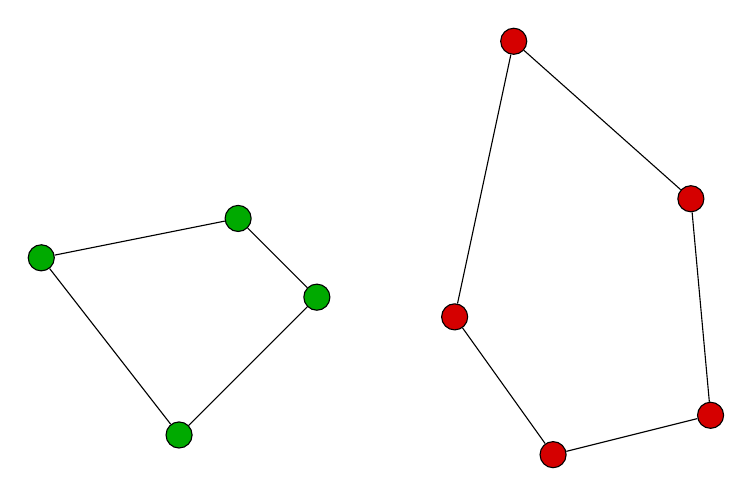
\begin{tikzpicture}
                % Node styles
                \tikzstyle{green}=[fill={rgb,255: red,0; green,170; blue,0}, draw=black, shape=circle]
                \tikzstyle{red}=[fill={rgb,255: red,213; green,0; blue,0}, draw=black, shape=circle]

                \node [style=green] (0) at (-0.75, 1) {};
                \node [style=green] (1) at (-3.25, 0.5) {};
                \node [style=green] (2) at (0.25, 0) {};
                \node [style=green] (3) at (-1.5, -1.75) {};
                \node [style=red] (4) at (2, -0.25) {};
                \node [style=red] (5) at (3.25, -2) {};
                \node [style=red] (6) at (5.25, -1.5) {};
                \node [style=red] (7) at (5, 1.25) {};
                \node [style=red] (8) at (2.75, 3.25) {};
                \draw (1) to (0);
                \draw (0) to (2);
                \draw (2) to (3);
                \draw (3) to (1);
                \draw (4) to (5);
                \draw (5) to (6);
                \draw (6) to (7);
                \draw (7) to (8);
                \draw (8) to (4);
            \end{tikzpicture}
        \end{center}
        \item \textbf{Łącz}

        Połącz wypukłe otoczki podzbiorów.

        Złożoność obliczeniowa: $O(n)$.

        \begin{center}
            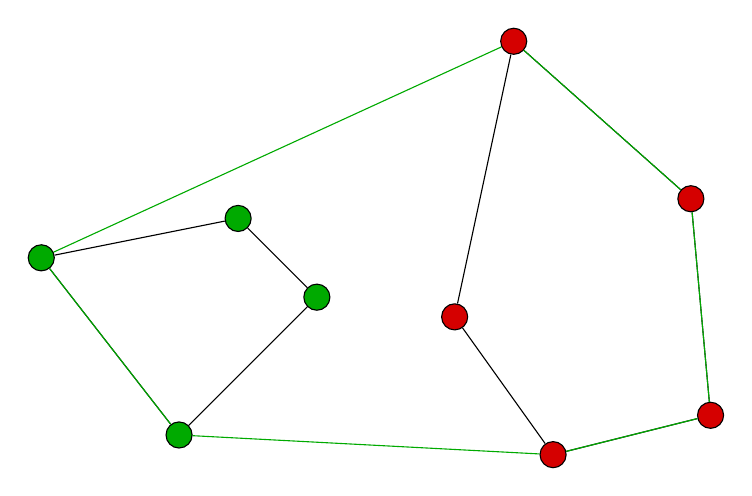
\begin{tikzpicture}
                % Node styles
                \tikzstyle{green}=[fill={rgb,255: red,0; green,170; blue,0}, draw=black, shape=circle]
                \tikzstyle{red}=[fill={rgb,255: red,213; green,0; blue,0}, draw=black, shape=circle]
                \tikzstyle{white}=[fill=white, draw=white, shape=circle]

                % Edge styles
                \tikzstyle{green-line}=[-, draw={rgb,255: red,0; green,170; blue,0}]

                \node [style=green] (0) at (-0.75, 1) {};
                \node [style=green] (1) at (-3.25, 0.5) {};
                \node [style=green] (2) at (0.25, 0) {};
                \node [style=green] (3) at (-1.5, -1.75) {};
                \node [style=red] (4) at (2, -0.25) {};
                \node [style=red] (5) at (3.25, -2) {};
                \node [style=red] (6) at (5.25, -1.5) {};
                \node [style=red] (7) at (5, 1.25) {};
                \node [style=red] (8) at (2.75, 3.25) {};
                \draw (1) to (0);
                \draw (0) to (2);
                \draw (2) to (3);
                \draw (3) to (1);
                \draw (4) to (5);
                \draw (5) to (6);
                \draw (6) to (7);
                \draw (7) to (8);
                \draw (8) to (4);
                \draw [style=green-line] (1) to (8);
                \draw [style=green-line] (3) to (5);
                \draw [style=green-line] (1) to (3);
                \draw [style=green-line] (8) to (7);
                \draw [style=green-line] (7) to (6);
                \draw [style=green-line] (6) to (5);
            \end{tikzpicture}
        \end{center}

        \begin{enumerate}
            \item Znajdź element $l_1$ ($r_1$) będący elementem wysuniętym najbardziej na
            lewo (prawo) w zbiorze $L$ ($R$)
            \begin{center}
                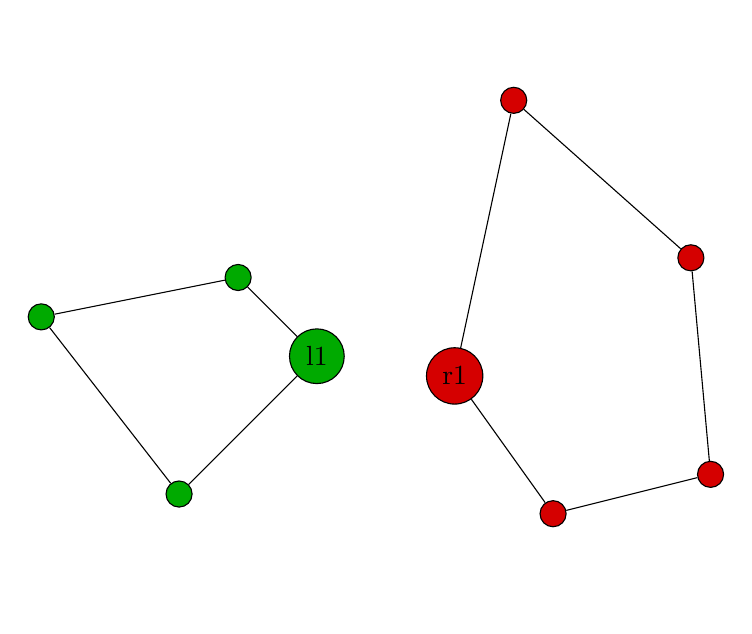
\begin{tikzpicture}
                    % Node styles
                    \tikzstyle{green}=[fill={rgb,255: red,0; green,170; blue,0}, draw=black, shape=circle]
                    \tikzstyle{red}=[fill={rgb,255: red,213; green,0; blue,0}, draw=black, shape=circle]
                    \tikzstyle{white}=[fill=white, draw=white, shape=circle]

                    % Edge styles
                    \tikzstyle{green-line}=[-, draw={rgb,255: red,0; green,170; blue,0}]
                    \tikzstyle{red-line}=[-, draw={rgb,255: red,213; green,0; blue,0}]
                    \node [style=green] (0) at (-0.75, 1) {};
                    \node [style=green] (1) at (-3.25, 0.5) {};
                    \node [style=green] (2) at (0.25, 0) {l1};
                    \node [style=green] (3) at (-1.5, -1.75) {};
                    \node [style=red] (4) at (2, -0.25) {r1};
                    \node [style=red] (5) at (3.25, -2) {};
                    \node [style=red] (6) at (5.25, -1.5) {};
                    \node [style=red] (7) at (5, 1.25) {};
                    \node [style=red] (8) at (2.75, 3.25) {};
                    \node [style=white] (9) at (1, -3) {};
                    \node [style=white] (10) at (1, 4) {};
                    \draw (1) to (0);
                    \draw (0) to (2);
                    \draw (2) to (3);
                    \draw (3) to (1);
                    \draw (4) to (5);
                    \draw (5) to (6);
                    \draw (6) to (7);
                    \draw (7) to (8);
                    \draw (8) to (4);
                \end{tikzpicture}
            \end{center}

            \item Znajdź elementy "górne" w $L$ i $R$, tzn. $l_u$ i $r_u$ dające wypukłą otoczkę,
            zaczynając od $l_1$ ($r_1$) i idąc przeciwnie (zgodnie z) do wskazówek zegara.
            \begin{center}
                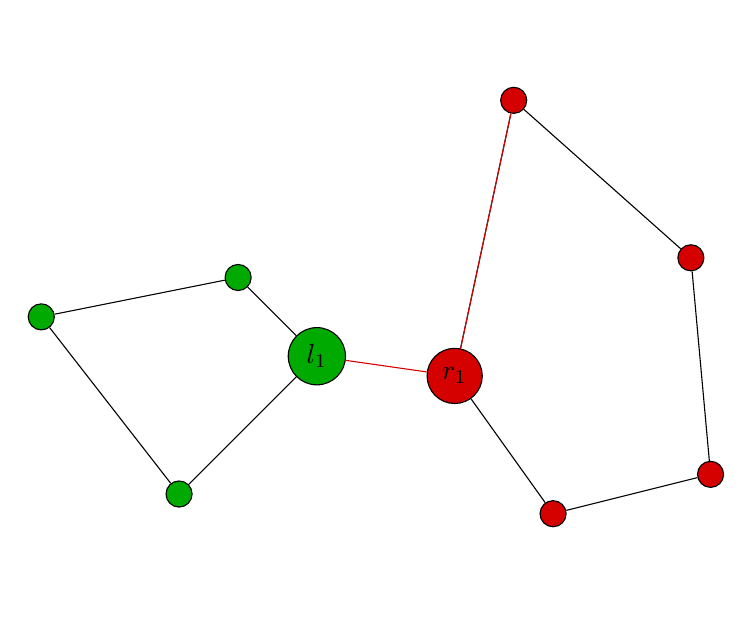
\begin{tikzpicture}
                    % Node styles
                    \tikzstyle{green}=[fill={rgb,255: red,0; green,170; blue,0}, draw=black, shape=circle]
                    \tikzstyle{red}=[fill={rgb,255: red,213; green,0; blue,0}, draw=black, shape=circle]
                    \tikzstyle{white}=[fill=white, draw=white, shape=circle]

                    % Edge styles
                    \tikzstyle{green-line}=[-, draw={rgb,255: red,0; green,170; blue,0}]
                    \tikzstyle{red-line}=[-, draw={rgb,255: red,213; green,0; blue,0}]

                    \node [style=green] (0) at (-0.75, 1) {};
                    \node [style=green] (1) at (-3.25, 0.5) {};
                    \node [style=green] (2) at (0.25, 0) {$l_1$};
                    \node [style=green] (3) at (-1.5, -1.75) {};
                    \node [style=red] (4) at (2, -0.25) {$r_1$};
                    \node [style=red] (5) at (3.25, -2) {};
                    \node [style=red] (6) at (5.25, -1.5) {};
                    \node [style=red] (7) at (5, 1.25) {};
                    \node [style=red] (8) at (2.75, 3.25) {};
                    \node [style=white] (9) at (1, -3) {};
                    \node [style=white] (10) at (1, 4) {};
                    \draw (1) to (0);
                    \draw (0) to (2);
                    \draw (2) to (3);
                    \draw (3) to (1);
                    \draw (4) to (5);
                    \draw (5) to (6);
                    \draw (6) to (7);
                    \draw (7) to (8);
                    \draw (8) to (4);
                    \draw [style=red-line] (2) to (4);
                    \draw [style=red-line] (4) to (8);
                \end{tikzpicture}

                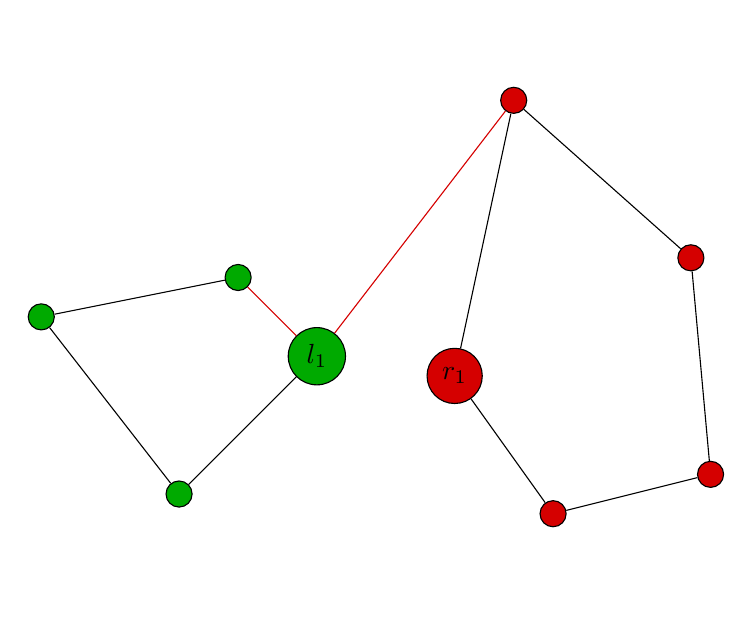
\begin{tikzpicture}
                    % Node styles
                    \tikzstyle{green}=[fill={rgb,255: red,0; green,170; blue,0}, draw=black, shape=circle]
                    \tikzstyle{red}=[fill={rgb,255: red,213; green,0; blue,0}, draw=black, shape=circle]
                    \tikzstyle{white}=[fill=white, draw=white, shape=circle]

                    % Edge styles
                    \tikzstyle{green-line}=[-, draw={rgb,255: red,0; green,170; blue,0}]
                    \tikzstyle{red-line}=[-, draw={rgb,255: red,213; green,0; blue,0}]
                    \node [style=green] (0) at (-0.75, 1) {};
                    \node [style=green] (1) at (-3.25, 0.5) {};
                    \node [style=green] (2) at (0.25, 0) {$l_1$};
                    \node [style=green] (3) at (-1.5, -1.75) {};
                    \node [style=red] (4) at (2, -0.25) {$r_1$};
                    \node [style=red] (5) at (3.25, -2) {};
                    \node [style=red] (6) at (5.25, -1.5) {};
                    \node [style=red] (7) at (5, 1.25) {};
                    \node [style=red] (8) at (2.75, 3.25) {};
                    \node [style=white] (9) at (1, -3) {};
                    \node [style=white] (10) at (1, 4) {};
                    \draw (1) to (0);
                    \draw (2) to (3);
                    \draw (3) to (1);
                    \draw (4) to (5);
                    \draw (5) to (6);
                    \draw (6) to (7);
                    \draw (7) to (8);
                    \draw [style=red-line] (2) to (8);
                    \draw [style=red-line] (0) to (2);
                    \draw  (8) to (4);
                \end{tikzpicture}

                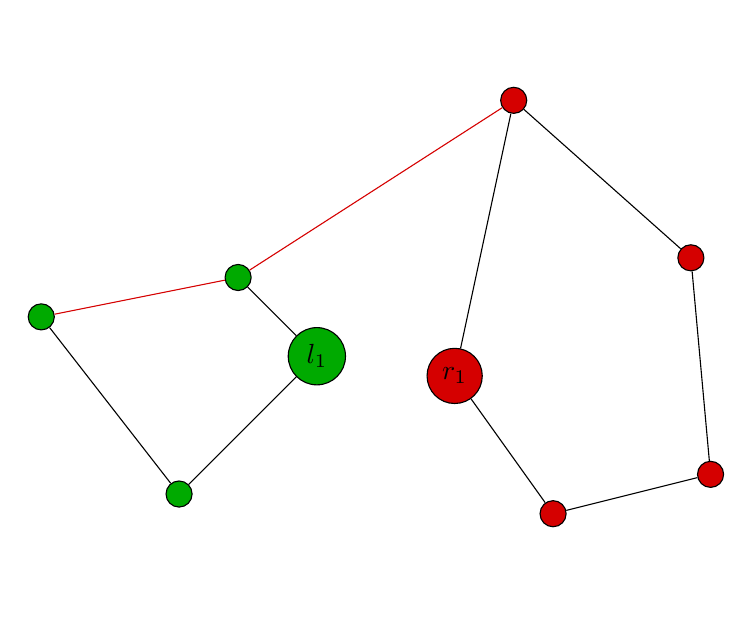
\begin{tikzpicture}
                    % Node styles
                    \tikzstyle{green}=[fill={rgb,255: red,0; green,170; blue,0}, draw=black, shape=circle]
                    \tikzstyle{red}=[fill={rgb,255: red,213; green,0; blue,0}, draw=black, shape=circle]
                    \tikzstyle{white}=[fill=white, draw=white, shape=circle]

                    % Edge styles
                    \tikzstyle{green-line}=[-, draw={rgb,255: red,0; green,170; blue,0}]
                    \tikzstyle{red-line}=[-, draw={rgb,255: red,213; green,0; blue,0}]

                    \node [style=green] (0) at (-0.75, 1) {};
                    \node [style=green] (1) at (-3.25, 0.5) {};
                    \node [style=green] (2) at (0.25, 0) {$l_1$};
                    \node [style=green] (3) at (-1.5, -1.75) {};
                    \node [style=red] (4) at (2, -0.25) {$r_1$};
                    \node [style=red] (5) at (3.25, -2) {};
                    \node [style=red] (6) at (5.25, -1.5) {};
                    \node [style=red] (7) at (5, 1.25) {};
                    \node [style=red] (8) at (2.75, 3.25) {};
                    \node [style=white] (9) at (1, -3) {};
                    \node [style=white] (10) at (1, 4) {};
                    \draw (2) to (3);
                    \draw (3) to (1);
                    \draw (4) to (5);
                    \draw (5) to (6);
                    \draw (6) to (7);
                    \draw (7) to (8);
                    \draw (8) to (4);
                    \draw [style=red-line] (1) to (0);
                    \draw [style=red-line] (0) to (8);
                    \draw (2) to (0);
                \end{tikzpicture}

                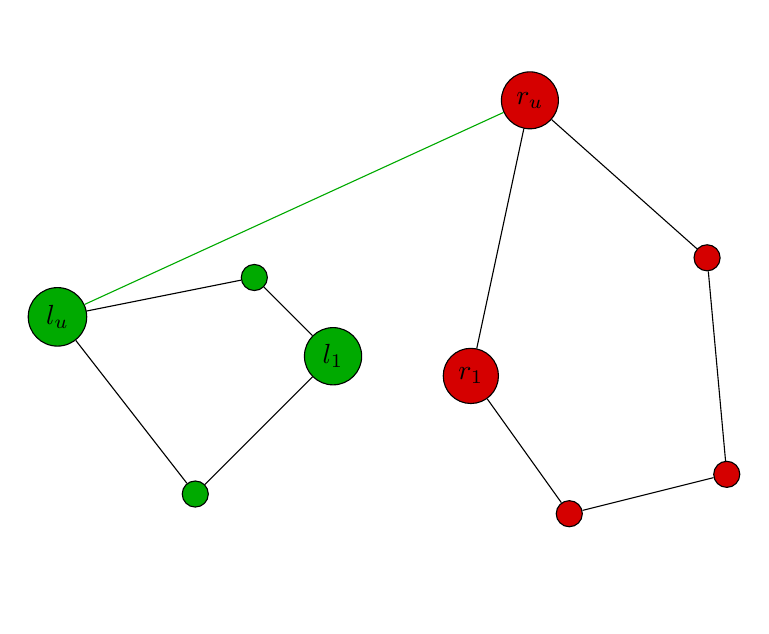
\begin{tikzpicture}
                    % Node styles
                    \tikzstyle{green}=[fill={rgb,255: red,0; green,170; blue,0}, draw=black, shape=circle]
                    \tikzstyle{red}=[fill={rgb,255: red,213; green,0; blue,0}, draw=black, shape=circle]
                    \tikzstyle{white}=[fill=white, draw=white, shape=circle]

                    % Edge styles
                    \tikzstyle{green-line}=[-, draw={rgb,255: red,0; green,170; blue,0}]
                    \tikzstyle{red-line}=[-, draw={rgb,255: red,213; green,0; blue,0}]

                    \node [style=green] (0) at (-0.75, 1) {};
                    \node [style=green] (1) at (-3.25, 0.5) {$l_u$};
                    \node [style=green] (2) at (0.25, 0) {$l_1$};
                    \node [style=green] (3) at (-1.5, -1.75) {};
                    \node [style=red] (4) at (2, -0.25) {$r_1$};
                    \node [style=red] (5) at (3.25, -2) {};
                    \node [style=red] (6) at (5.25, -1.5) {};
                    \node [style=red] (7) at (5, 1.25) {};
                    \node [style=red] (8) at (2.75, 3.25) {$r_u$};
                    \node [style=white] (9) at (1, -3) {};
                    \node [style=white] (10) at (1, 4) {};
                    \draw (1) to (0);
                    \draw (0) to (2);
                    \draw (2) to (3);
                    \draw (3) to (1);
                    \draw (4) to (5);
                    \draw (5) to (6);
                    \draw (6) to (7);
                    \draw (7) to (8);
                    \draw (8) to (4);
                    \draw [style=green-line] (1) to (8);
                \end{tikzpicture}

            \end{center}
            \item Analogicznie znajdź $l_d$ i $r_d$

            \begin{center}
                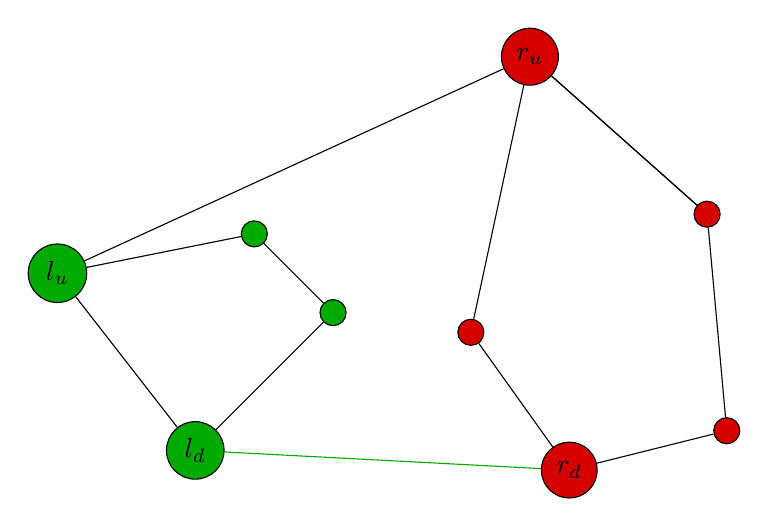
\begin{tikzpicture}
                    % Node styles
                    \tikzstyle{green}=[fill={rgb,255: red,0; green,170; blue,0}, draw=black, shape=circle]
                    \tikzstyle{red}=[fill={rgb,255: red,213; green,0; blue,0}, draw=black, shape=circle]
                    \tikzstyle{white}=[fill=white, draw=white, shape=circle]

                    % Edge styles
                    \tikzstyle{green-line}=[-, draw={rgb,255: red,0; green,170; blue,0}]

                    \node [style=green] (0) at (-0.75, 1) {};
                    \node [style=green] (1) at (-3.25, 0.5) {$l_u$};
                    \node [style=green] (2) at (0.25, 0) {};
                    \node [style=green] (3) at (-1.5, -1.75) {$l_d$};
                    \node [style=red] (4) at (2, -0.25) {};
                    \node [style=red] (5) at (3.25, -2) {$r_d$};
                    \node [style=red] (6) at (5.25, -1.5) {};
                    \node [style=red] (7) at (5, 1.25) {};
                    \node [style=red] (8) at (2.75, 3.25) {$r_u$};
                    \draw (0) to (2);
                    \draw (2) to (3);
                    \draw (3) to (1);
                    \draw (4) to (5);
                    \draw (5) to (6);
                    \draw (6) to (7);
                    \draw (7) to (8);
                    \draw (8) to (4);
                    \draw (1) to (8);
                    \draw (1) to (0);
                    \draw (8) to (7);
                    \draw [style=green-line] (3) to (5);
                \end{tikzpicture}
            \end{center}
            \item Zwróć otoczkę składającą się z:
            \begin{itemize}
                \item krawędzi $l_u$ - $r_u$
                \item fragmentu otoczki $R$ łączącej $r_u$ z $r_l$
                \item krawędzi $r_d$ - $l_d$
                \item fragmentu otoczki $L$ łączącej $l_d$ z $l_u$
            \end{itemize}

            \begin{center}
                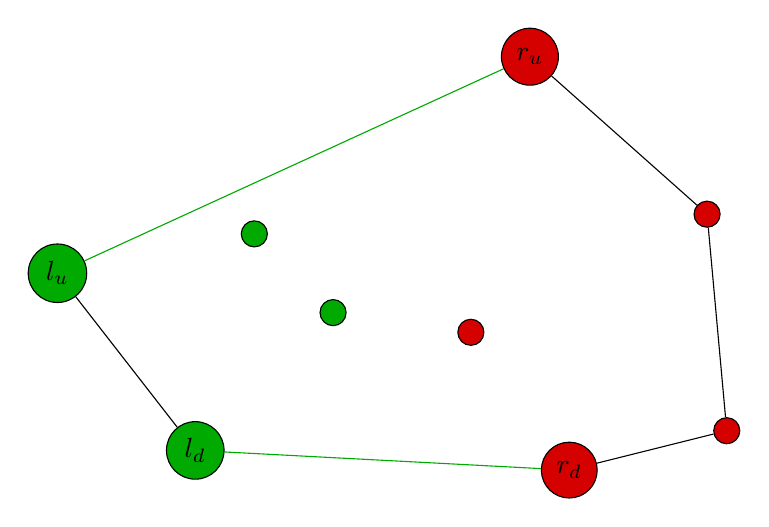
\begin{tikzpicture}
                    % Node styles
                    \tikzstyle{green}=[fill={rgb,255: red,0; green,170; blue,0}, draw=black, shape=circle]
                    \tikzstyle{red}=[fill={rgb,255: red,213; green,0; blue,0}, draw=black, shape=circle]

                    % Edge styles
                    \tikzstyle{green-line}=[-, draw={rgb,255: red,0; green,170; blue,0}]
                    \tikzstyle{red-line}=[-, draw={rgb,255: red,213; green,0; blue,0}]

                    \node [style=green] (0) at (-0.75, 1) {};
                    \node [style=green] (1) at (-3.25, 0.5) {$l_u$};
                    \node [style=green] (2) at (0.25, 0) {};
                    \node [style=green] (3) at (-1.5, -1.75) {$l_d$};
                    \node [style=red] (4) at (2, -0.25) {};
                    \node [style=red] (5) at (3.25, -2) {$r_d$};
                    \node [style=red] (6) at (5.25, -1.5) {};
                    \node [style=red] (7) at (5, 1.25) {};
                    \node [style=red] (8) at (2.75, 3.25) {$r_u$};
                    \draw (3) to (1);
                    \draw (5) to (6);
                    \draw (6) to (7);
                    \draw (7) to (8);
                    \draw [style=green-line] (1) to (8);
                    \draw [style=green-line] (3) to (5);
                \end{tikzpicture}

            \end{center}
        \end{enumerate}
    \end{enumerate}
    \[\]
    \textbf{Złożoność algorytmu:} $\theta(n \cdot \log(n))$. \[\]
    \textbf{Uzasadnienie:} podział na 2 podproblemy (z podziałem i łączeniem zajmującym
    $O(n)$ czasu): $O(n \cdot \log(n))$ + złożoność sortowania punktów wg. osi $x$
    ($\theta(n \cdot \log(n)$), co daje razem $\theta(n \cdot \log(n))$.
    \newpage

    \section{Lista: ujęcie abstrakcyjne, możliwe implementacje i ich złożoności.}
    \section{Kolejka i kolejka priorytetowa: ujęcie abstrakcyjne, możliwe implementacje i ich złożoności.}
    \section{Algorytmy sortowania QuickSort i MergeSort: metody wyboru pivota w QS; złożoności.}
    \section{Algorytm sortowania bez porównań (sortowanie przez zliczanie, sortowanie kubełkowe oraz sortowanie pozycyjne).}

    \newpage

    \section{Reprezentacja drzewa binarnego za pomocą porządków (preorder, inorder, postorder).}

    \begin{center}
        \begin{forest}
            for tree={circle,draw}
            [22
            [13
            [30
            [15]
            [85]]
            [71
            [17]
            [20]]]
            [11
            [32
            [33]
            [,.phantom]]
            [55]]]
        \end{forest}
    \end{center}

    \noindent \textbf{Preorder}: 22, 13, 30, 15, 85, 71, 17, 20, 11, 32, 33, 55\\
    \textbf{Inorder}: 15, 30, 85, 13, 17, 71, 20, 22, 33, 32, 11, 55\\
    \textbf{Postorder}: 15, 85, 30, 17, 20, 71, 13, 33, 32, 55, 11, 22\\

    \subsection{Odtworzenie drzewa z preordera i inordera.}
    Idea algorytmu:
    \begin{enumerate}
        \item Element pierwszy w preorderze to korzeń.
        \item Znalezienie tego elementu w inorderze dzieli go na dwie części - elementy po lewej stanowią jego
        lewe poddrzewo, po prawej - prawe.
        \item Rekurencyjnie budujemy kolejne poddrzewa.
    \end{enumerate}

    \noindent \textbf{Preorder}:  \textbf{22}, 13, 30, 15, 85, 71, 17, 20, 11, 32, 33, 55\\
    \textbf{Inorder}: 15, 30, 85, 13, 17, 71, 20, \textbf{22}, 33, 32, 11, 55\\

    \begin{center}
        \begin{forest}
            for tree={circle,draw}
            [22
            [$L_1$]
            [$P_1$]]
        \end{forest}
    \end{center}
    Gdzie $L_1$ = lewe poddrzewo zawierające elementy 15, 30, 85, 13, 17, 71, 20, $P_1$ - prawe poddrzewo zawierające
    33, 32, 11, 55.\\

    \noindent Budujemy rekurencyjnie $L_1$.\\
    \textbf{Preorder}:  \textbf{13}, 30, 15, 85, 71, 17, 20\\
    \textbf{Inorder}: 15, 30, 85, \textbf{13}, 17, 71, 20\\

    \begin{center}
        \begin{forest}
            for tree={circle,draw}
            [22
            [13
            [$L_2$]
            [$P_2$]]
            [$P_1$]]
        \end{forest}
    \end{center}
    $L_2$ = 15, 30, 85; $P_2$ = 17, 71, 20.\\

    \noindent Budujemy rekurencyjnie $L_2$.\\
    \textbf{Preorder}: \textbf{30}, 15, 85\\
    \textbf{Inorder}: 15, \textbf{30}, 85\\

    \begin{center}
        \begin{forest}
            for tree={circle,draw}
            [22
            [13
            [30
            [15]
            [85]]
            [$P_2$]]
            [$P_1$]]
        \end{forest}
    \end{center}
    \hfill \\

    \noindent Budujemy rekurencyjnie $P_2$.\\
    \textbf{Preorder}: \textbf{71}, 17, 20\\
    \textbf{Inorder}: 17, \textbf{71}, 20\\

    \begin{center}
        \begin{forest}
            for tree={circle,draw}
            [22
            [13
            [30
            [15]
            [85]]
            [71
            [17]
            [20]]]
            [$P_1$]]
        \end{forest}
    \end{center}
    \hfill \\

    \noindent Budujemy rekurencyjnie $P_1$.\\
    \textbf{Preorder}:  \textbf{11}, 32, 33, 55\\
    \textbf{Inorder}: 33, 32, \textbf{11}, 55\\

    \begin{center}
        \begin{forest}
            for tree={circle,draw}
            [22
            [13
            [30
            [15]
            [85]]
            [71
            [17]
            [20]]]
            [11
            [$L_3$]
            [55]]]
        \end{forest}
    \end{center}
    Gdzie $L_3$ = 32, 33.\\

    \noindent Budujemy rekurencyjnie $L_3$.\\
    \textbf{Preorder}:  \textbf{32}, 33\\
    \textbf{Inorder}: 33, \textbf{32}\\

    \begin{center}
        \begin{forest}
            for tree={circle,draw}
            [22
            [13
            [30
            [15]
            [85]]
            [71
            [17]
            [20]]]
            [11
            [32
            [33]
            [,.phantom]]
            [55]]]
        \end{forest}
    \end{center}

    Odbudowaliśmy drzewo wyjściowe.\\

    Odtworzenie drzewa z postordera i inordera jest kompletnie analogiczne, z dokładnością do przeglądania postordera
    od końca i budowania rekurencyjnie najpierw prawych, potem lewych poddrzew. Cała logika jest identyczna.


    \newpage

    \section{Algorytmy wyszukiwania następnika i poprzednika w drzewach BST; usuwanie węzła.}

    \subsection{Wyszukiwanie następnika i poprzednika w BST.}

    \begin{center}
        \begin{forest}
            for tree={circle,draw}
            [8
            [3
            [1
            [,.phantom]
            [,.phantom]]
            [6
            [4]
            [7]]]
            [10
            [,.phantom
            [,.phantom]
            [,.phantom]]
            [14
            [13]
            [,.phantom]]]]
        \end{forest}
    \end{center}

    Rodzaje następników:
    \begin{enumerate}
        \item skrajnie lewy element prawego poddrzewa węzła, jeśli posiada on prawe poddrzewo, np:
        \begin{itemize}
            \item 4 jest następnikiem 3,
            \item 10 jest następnikiem 8,
            \item 13 jest następnikiem 10.
        \end{itemize}
        \item pierwszy napotkany przodek węzła, dla którego węzeł jest w lewym poddrzewie, np:
        \begin{itemize}
            \item 3 jest następnikiem 1,
            \item 8 jest następnikiem 7,
            \item 14 jest następnikiem 13.
        \end{itemize}
    \end{enumerate}

    Rodzaje poprzedników:
    \begin{enumerate}
        \item skrajnie prawy element lewego poddrzewa węzła, jeśli posiada on lewe poddrzewo, np:
        \begin{itemize}
            \item 7 jest poprzednikiem 8,
            \item 1 jest poprzednikiem 3,
            \item 13 jest poprzednikiem 14.
        \end{itemize}
        \item pierwszy napotkany przodek węzła, dla którego węzeł jest w prawym poddrzewie, np:
        \begin{itemize}
            \item 6 jest poprzednikiem 7,
            \item 10 jest poprzednikiem 13,
            \item 8 jest poprzednikiem 10.
        \end{itemize}
    \end{enumerate}

    \subsection{Usuwanie węzła z BST.}

    Przypadki usuwania węzła:
    \begin{enumerate}
        \item usuwanie liścia, np. 13:
        \begin{center}
            \begin{forest}
                for tree={circle,draw}
                [8
                [3
                [1
                [,.phantom]
                [,.phantom]]
                [6
                [4]
                [7]]]
                [10
                [,.phantom
                [,.phantom]
                [,.phantom]]
                [14
                [13, draw={red}]
                [,.phantom]]]]
            \end{forest}
            \begin{forest}
                for tree={circle,draw}
                [8
                [3
                [1
                [,.phantom]
                [,.phantom]]
                [6
                [4]
                [7]]]
                [10
                [,.phantom
                [,.phantom]
                [,.phantom]]
                [14
                [,.phantom]
                [,.phantom]]]]
            \end{forest}
        \end{center}
        \item usuwanie węzła z jednym synem, np. 14:
        \begin{center}
            \begin{forest}
                for tree={circle,draw}
                [8
                [3
                [1
                [,.phantom]
                [,.phantom]]
                [6
                [4]
                [7]]]
                [10
                [,.phantom
                [,.phantom]
                [,.phantom]]
                [14, draw={red}
                [13]
                [,.phantom]]]]
            \end{forest}
            \begin{forest}
                for tree={circle,draw}
                [8
                [3
                [1
                [,.phantom]
                [,.phantom]]
                [6
                [4]
                [7]]]
                [10
                [,.phantom
                [,.phantom]
                [,.phantom]]
                [13, draw={red}, edge={red}
                [,.phantom]
                [,.phantom]]]]
            \end{forest}
        \end{center}
        \item usuwanie węzła z dwoma synami, np 3 (następnikiem 3 jest 4):
        \begin{center}
            \begin{forest}
                for tree={circle,draw}
                [8
                [3, draw={red}
                [1
                [,.phantom]
                [,.phantom]]
                [6
                [4]
                [7]]]
                [10
                [,.phantom
                [,.phantom]
                [,.phantom]]
                [14
                [13]
                [,.phantom]]]]
            \end{forest}
            \begin{forest}
                for tree={circle,draw}
                [8
                [4, draw={red}
                [1
                [,.phantom]
                [,.phantom]]
                [6
                [,.phantom]
                [7]]]
                [10
                [,.phantom
                [,.phantom]
                [,.phantom]]
                [14
                [13]
                [,.phantom]]]]
            \end{forest}
        \end{center}
    \end{enumerate}

    \newpage

    \section{B-drzewa: operacje i ich złożoność.}
    Wszystkie operacje są przeprowadzane na drzewie rzędu 3.

    \subsection{Wyszukiwanie}
    Wyszukanie elementu \texttt{0003} w drzewie.

    \begin{center}
        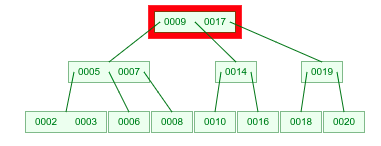
\includegraphics[width=0.7\linewidth]{b-trees/find/find-1.png} \\
        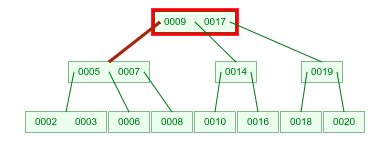
\includegraphics[width=0.7\linewidth]{b-trees/find/find-2.png} \\
        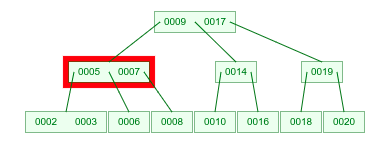
\includegraphics[width=0.7\linewidth]{b-trees/find/find-3.png} \\
        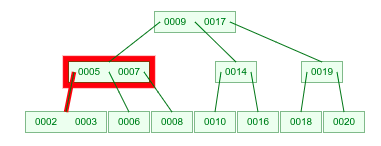
\includegraphics[width=0.7\linewidth]{b-trees/find/find-4.png} \\
        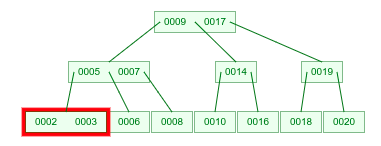
\includegraphics[width=0.7\linewidth]{b-trees/find/find-5.png} \\
        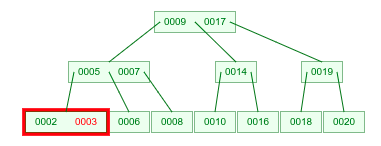
\includegraphics[width=0.7\linewidth]{b-trees/find/find-6.png} \\
    \end{center}

    \subsection{Wstawianie}
    Wstawianie elementu \texttt{0030} do poniższego drzewa: \\
    
\includegraphics[width=\linewidth]{b-trees/insert/begin.png} \\

    \noindent Wyszukujemy liść, do którego mamy wstawić element: \\
    \includegraphics[width=\linewidth]{b-trees/insert/find-01.png} \\
    \includegraphics[width=\linewidth]{b-trees/insert/find-02.png} \\
    \includegraphics[width=\linewidth]{b-trees/insert/find-03.png} \\
    \includegraphics[width=\linewidth]{b-trees/insert/find-04.png} \\
    \includegraphics[width=\linewidth]{b-trees/insert/find-05.png} \\

    \noindent Następnie wstawiamy nasz element: \\
    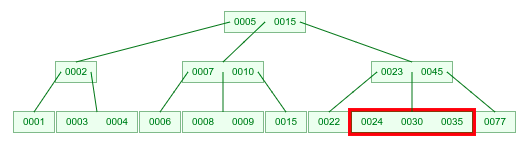
\includegraphics[width=\linewidth]{b-trees/insert/insert.png} \\

    \noindent Ponieważ liść, do którego wstawiliśmy element nie spełnia warunków drzewa ($3 \geq K=3$) musimy zbalansować drzewo. Bierzemy więc środkowy element z naszego liścia i przenosimy do rodzica, a jako jego potomków ustawiamy odpowiednio obie części podzielonego oryginalnego liścia: \\
    \includegraphics[width=\linewidth]{b-trees/insert/rebalance-01.png} \\

    \noindent Okazuje się, że po tej operacji nasz rodzic nie spełnia założenia drzewa. Stosujemy więc wobec niego podobną operację: \\
    \includegraphics[width=\linewidth]{b-trees/insert/rebalance-02.png} \\
    \includegraphics[width=\linewidth]{b-trees/insert/rebalance-03.png} \\

    \noindent Następnie okazuje się, że i w korzeniu warunki drzewa są zaburzone. Zwiększamy więc głębokość drzewa dzieląc dotychczasowy korzeń na dwa względem środkowego elementu i czyniąc z nich potomków środkowego elementu, który staje się teraz nowym korzeniem: \\
    \includegraphics[width=\linewidth]{b-trees/insert/rebalance-04.png} \\
    \includegraphics[width=\linewidth]{b-trees/insert/rebalance-05.png} \\

    \noindent Teraz drzewo jest zbalansowane

    \subsection{Usuwanie}
    Usuwanie elementu \texttt{0023} z drzewa: \\
    
\includegraphics[width=\linewidth]{b-trees/delete/begin.png} \\

    \noindent Wyszukujemy element do usunięcia: \\
    \includegraphics[width=\linewidth]{b-trees/delete/find-01.png} \\
    \includegraphics[width=\linewidth]{b-trees/delete/find-02.png} \\
    \includegraphics[width=\linewidth]{b-trees/delete/find-03.png} \\
    \includegraphics[width=\linewidth]{b-trees/delete/find-04.png} \\
    \includegraphics[width=\linewidth]{b-trees/delete/find-05.png} \\

    \noindent Usuwamy element: \\
    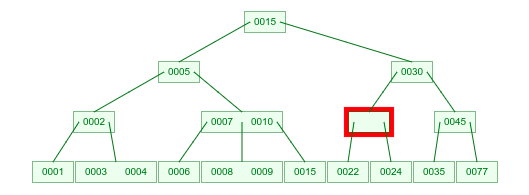
\includegraphics[width=\linewidth]{b-trees/delete/delete.png} \\

    \noindent Usunięty element zastępujemy największym elementem z lewego poddrzewa: \\
    \includegraphics[width=\linewidth]{b-trees/delete/rebalance-01.png} \\

    \noindent Ponieważ warunki drzewa nie są zachowane dla węzła z przedostatniego poziomu ($1 < \lceil K/2 \rceil = 2$ - minimalna ilość potomków - lewy liść w praktyce nie istnieje) musimy zbalansować drzewo: \\
    \includegraphics[width=\linewidth]{b-trees/delete/rebalance-02.png} \\
    \includegraphics[width=\linewidth]{b-trees/delete/rebalance-03.png} \\
    \includegraphics[width=\linewidth]{b-trees/delete/rebalance-04.png} \\
    \includegraphics[width=\linewidth]{b-trees/delete/rebalance-05.png} \\

    \noindent To samo musimy przeprowadzić dla wyższego poziomu: \\
    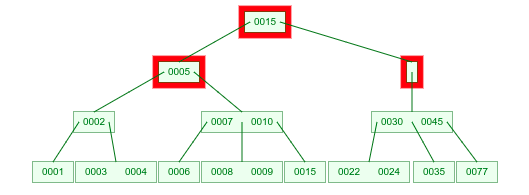
\includegraphics[width=\linewidth]{b-trees/delete/rebalance-06.png} \\
    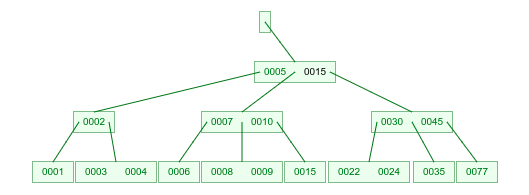
\includegraphics[width=\linewidth]{b-trees/delete/rebalance-07.png} \\
    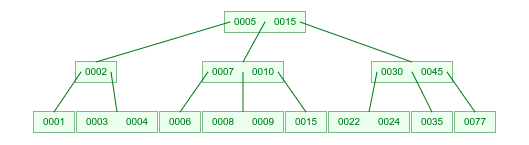
\includegraphics[width=\linewidth]{b-trees/delete/rebalance-08.png} \\

    \noindent Teraz drzewo jest zbalansowane \\

    \noindent \textbf{Link do symulatora: \url{https://www.cs.usfca.edu/~galles/visualization/BTree.html}}

    \newpage


    \section{Drzewa AVL: rotacje, operacje z wykorzystaniem rotacji i ich złożoność.}
    \subsection{Wstawianie}
    Wstawiamy po kolei elementy: 10, 5, 2, 4, 3 \\

    \noindent Wstawianie 2 pierwszych elementów przebiega dokładnie tak, jak dla zwykłego drzewa BST - równoważenie nie jest wymagane. Po wstawieniu 3 elementu tą samą metodą dostajemy następujące drzewo: \\

    \begin{center}
        \begin{forest}
            for tree={circle,draw}
            [10
            [5
            [2][,.phantom]
            [,.phantom]]
            [,.phantom]]
        \end{forest}
    \end{center}

    Ponieważ dla węzła \texttt{10} lewe poddrzewo jest o 2 głębsze niż prawe poddrzewo, musimy zastosować rotację. Na pierwszym poziomie mamy głębsze lewe poddrzewo, na drugim podobnie, musimy więc zastosować rotację LL: \\

    \begin{center}
        \begin{forest}
            for tree={circle,draw}
            [5
            [2]
            [10]]
        \end{forest}
    \end{center}

    Następnie wstawiamy element \texttt{4} - równoważenie nie jest potrzebne. Wstawiamy element \texttt{3} i otrzymujemy następujące drzewo: \\

    \begin{center}
        \begin{forest}
            for tree={circle,draw}
            [5
            [2
            [,.phantom]
            [4
            [3][,.phantom]]]
            [10]]
        \end{forest}
    \end{center}

    Jak widać dla węzła \texttt{2} prawe poddrzewo jest o 2 głębsze niż lewe. Ponieważ na pierwszym poziomie (względem elementu \texttt{2}) mamy głębsze prawe poddrzewo, a na drugim lewe, musimy zastosować rotację RL: \\

    \noindent Pierwszy krok rotacji RL (doprowadzamy do sytuacji dla rotacji RR): \\

    \begin{center}
        \begin{forest}
            for tree={circle,draw}
            [5
            [2
            [,.phantom]
            [3
            [,.phantom][4]]]
            [10]]
        \end{forest}
    \end{center}

    Drugi krok rotacji RL (taki sam jak przy rotacji RR): \\

    \begin{center}
        \begin{forest}
            for tree={circle,draw}
            [5
            [3
            [2][4]]
            [10]]
        \end{forest}
    \end{center}

    Drzewo znów jest zrównoważone

    \subsection{Usuwanie}
    Z drzewa z poprzedniego przykładu usuniemy element \texttt{10}. Po jego usunięciu tak jak w przypadku zwykłego drzewa BST, otrzymujemy poniższe drzewo: \\

    \begin{center}
        \begin{forest}
            for tree={circle,draw}
            [5
            [3
            [2][4]]
            [,.phantom]]
        \end{forest}
    \end{center}

    Widzimy że dla węzła \texttt{5} drzewo jest niezrównoważone. Na pierwszym poziomie lewe poddrzewo jest głębsze. Na drugim poziomie oba poddrzewa mają tą samą głębokość - możemy więc zastosować prostszą wersję algorytmu rotacji - rotację LL (a nie rotację LR): \\

    \begin{center}
        \begin{forest}
            for tree={circle,draw}
            [3
            [2][,.phantom]
            [5
            [4][,.phantom]
            [,.phantom]]]
        \end{forest}
    \end{center}

    Teraz drzewo jest znów zrównoważone. \\

    \noindent \textbf{Link do symulatora: \url{https://www.cs.usfca.edu/~galles/visualization/AVLtree.html}}

    \newpage

    \section{Algorytmy przeszukiwania wszerz i wgłąb w grafach.}

    \subsection{Przeszukiwanie wszerz}

    \begin{center}

        \begin{gather*}
            S = \{s\}\\
            P = \{\}\\
        \end{gather*}
        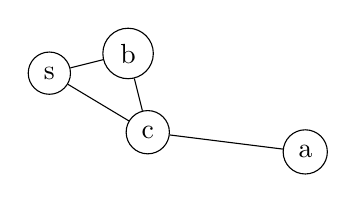
\begin{tikzpicture}
            \tikzstyle{white-fill}=[fill=white, draw=black, shape=circle]

            \node [style=white-fill] (0) at (-1.75, -0.25) {s};
            \node [style=white-fill] (2) at (-0.75, 0) {b};
            \node [style=white-fill] (3) at (-0.5, -1) {c};
            \node [style=white-fill] (4) at (1.5, -1.25) {a};
            \draw (0) to (2);
            \draw (0) to (3);
            \draw (3) to (4);
            \draw (2) to (3);
        \end{tikzpicture}

        \begin{gather*}
            S = \{b, c\}\\
            P = \{b : s, c : s\}\\
        \end{gather*}

        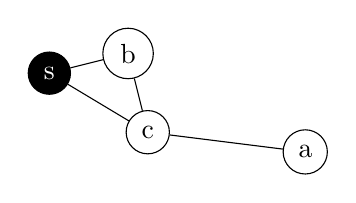
\begin{tikzpicture}
            \tikzstyle{white-fill}=[fill=white, draw=black, shape=circle]
            \tikzstyle{black-fill}=[fill=black, draw=black, shape=circle, text=white]

            \node [style=black-fill] (0) at (-1.75, -0.25) {s};
            \node [style=white-fill] (2) at (-0.75, 0) {b};
            \node [style=white-fill] (3) at (-0.5, -1) {c};
            \node [style=white-fill] (4) at (1.5, -1.25) {a};
            \draw (0) to (2);
            \draw (0) to (3);
            \draw (3) to (4);
            \draw (2) to (3);
        \end{tikzpicture}

        \begin{gather*}
            S = \{c\}\\
            P = \{b : s, c : s\}\\
        \end{gather*}

        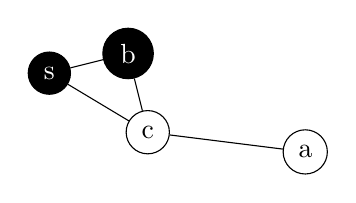
\begin{tikzpicture}
            \tikzstyle{white-fill}=[fill=white, draw=black, shape=circle]
            \tikzstyle{black-fill}=[fill=black, draw=black, shape=circle, text=white]

            \node [style=black-fill] (0) at (-1.75, -0.25) {s};
            \node [style=black-fill] (2) at (-0.75, 0) {b};
            \node [style=white-fill] (3) at (-0.5, -1) {c};
            \node [style=white-fill] (4) at (1.5, -1.25) {a};
            \draw (0) to (2);
            \draw (0) to (3);
            \draw (3) to (4);
            \draw (2) to (3);
        \end{tikzpicture}

        \begin{gather*}
            S = \{a\}\\
            P = \{b : s, c : s, a : c\}\\
        \end{gather*}

        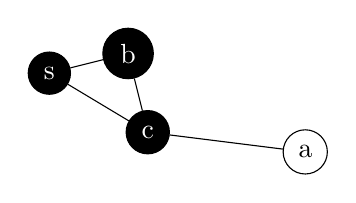
\begin{tikzpicture}
            \tikzstyle{white-fill}=[fill=white, draw=black, shape=circle]
            \tikzstyle{black-fill}=[fill=black, draw=black, shape=circle, text=white]

            \node [style=black-fill] (0) at (-1.75, -0.25) {s};
            \node [style=black-fill] (2) at (-0.75, 0) {b};
            \node [style=black-fill] (3) at (-0.5, -1) {c};
            \node [style=white-fill] (4) at (1.5, -1.25) {a};
            \draw (0) to (2);
            \draw (0) to (3);
            \draw (3) to (4);
            \draw (2) to (3);
        \end{tikzpicture}

        \begin{gather*}
            S = \{\}\\
            P = \{b : s, c : s, a : c\}\\
        \end{gather*}

        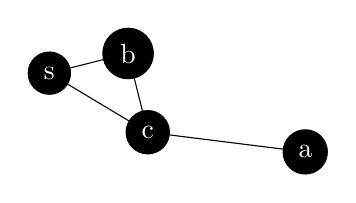
\begin{tikzpicture}
            \tikzstyle{white-fill}=[fill=white, draw=black, shape=circle]
            \tikzstyle{black-fill}=[fill=black, draw=black, shape=circle, text=white]

            \node [style=black-fill] (0) at (-1.75, -0.25) {s};
            \node [style=black-fill] (2) at (-0.75, 0) {b};
            \node [style=black-fill] (3) at (-0.5, -1) {c};
            \node [style=black-fill] (4) at (1.5, -1.25) {a};
            \draw (0) to (2);
            \draw (0) to (3);
            \draw (3) to (4);
            \draw (2) to (3);
        \end{tikzpicture}
    \end{center}

    \begin{center}

        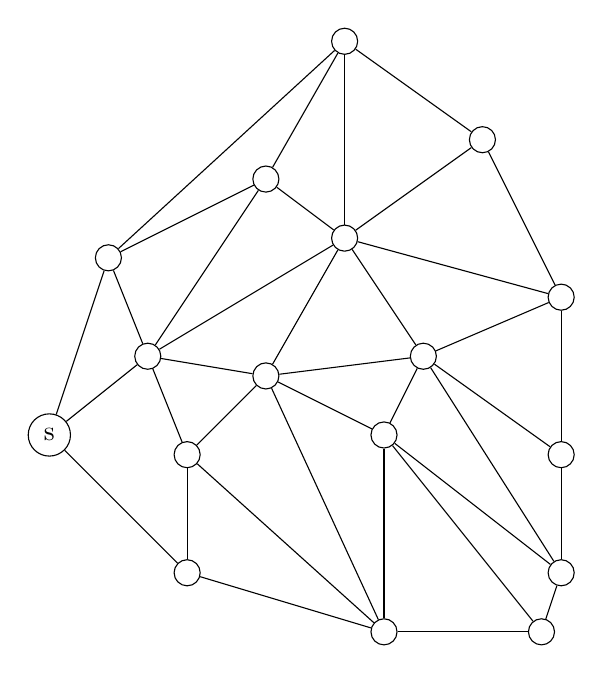
\begin{tikzpicture}
            \tikzstyle{white-fill}=[fill=white, draw=black, shape=circle]
            \tikzstyle{black-fill}=[fill=black, draw=black, shape=circle, text=white]

            \node [style=white-fill] (0) at (-2.25, -0.5) {s};
            \node [style=white-fill] (1) at (-1.5, 1.75) {};
            \node [style=white-fill] (2) at (0.5, 0.25) {};
            \node [style=white-fill] (3) at (-0.5, -0.75) {};
            \node [style=white-fill] (4) at (-0.5, -2.25) {};
            \node [style=white-fill] (5) at (-1, 0.5) {};
            \node [style=white-fill] (6) at (0.5, 2.75) {};
            \node [style=white-fill] (7) at (1.5, 2) {};
            \node [style=white-fill] (8) at (2.5, 0.5) {};
            \node [style=white-fill] (9) at (2, -0.5) {};
            \node [style=white-fill] (10) at (2, -3) {};
            \node [style=white-fill] (11) at (1.5, 4.5) {};
            \node [style=white-fill] (12) at (3.25, 3.25) {};
            \node [style=white-fill] (13) at (4.25, 1.25) {};
            \node [style=white-fill] (14) at (4.25, -0.75) {};
            \node [style=white-fill] (15) at (4.25, -2.25) {};
            \node [style=white-fill] (16) at (4, -3) {};
            \draw (1) to (0);
            \draw (5) to (3);
            \draw (0) to (5);
            \draw (0) to (4);
            \draw (4) to (10);
            \draw (3) to (2);
            \draw (11) to (1);
            \draw (5) to (7);
            \draw (6) to (7);
            \draw (6) to (11);
            \draw (6) to (1);
            \draw (7) to (12);
            \draw (11) to (12);
            \draw (7) to (8);
            \draw (7) to (2);
            \draw (2) to (10);
            \draw (2) to (9);
            \draw (8) to (9);
            \draw (3) to (4);
            \draw (9) to (16);
            \draw (10) to (16);
            \draw (8) to (15);
            \draw (15) to (16);
            \draw (8) to (14);
            \draw (14) to (13);
            \draw (13) to (7);
            \draw (8) to (13);
            \draw (15) to (14);
            \draw (3) to (10);
            \draw (9) to (10);
            \draw (5) to (2);
            \draw (5) to (1);
            \draw (5) to (6);
            \draw (2) to (8);
            \draw (11) to (7);
            \draw (12) to (13);
            \draw (9) to (15);
        \end{tikzpicture}

        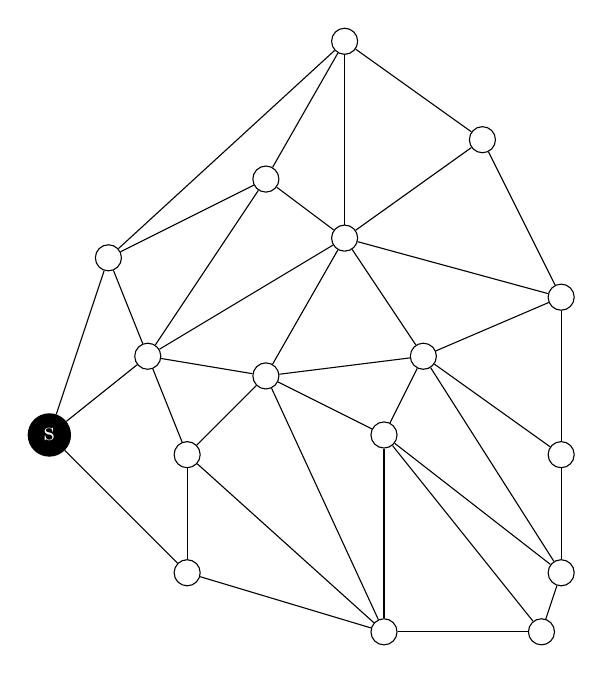
\begin{tikzpicture}
            \tikzstyle{white-fill}=[fill=white, draw=black, shape=circle]
            \tikzstyle{black-fill}=[fill=black, draw=black, shape=circle, text=white]
            \node [style=black-fill] (0) at (-2.25, -0.5) {s};
            \node [style=white-fill] (1) at (-1.5, 1.75) {};
            \node [style=white-fill] (2) at (0.5, 0.25) {};
            \node [style=white-fill] (3) at (-0.5, -0.75) {};
            \node [style=white-fill] (4) at (-0.5, -2.25) {};
            \node [style=white-fill] (5) at (-1, 0.5) {};
            \node [style=white-fill] (6) at (0.5, 2.75) {};
            \node [style=white-fill] (7) at (1.5, 2) {};
            \node [style=white-fill] (8) at (2.5, 0.5) {};
            \node [style=white-fill] (9) at (2, -0.5) {};
            \node [style=white-fill] (10) at (2, -3) {};
            \node [style=white-fill] (11) at (1.5, 4.5) {};
            \node [style=white-fill] (12) at (3.25, 3.25) {};
            \node [style=white-fill] (13) at (4.25, 1.25) {};
            \node [style=white-fill] (14) at (4.25, -0.75) {};
            \node [style=white-fill] (15) at (4.25, -2.25) {};
            \node [style=white-fill] (16) at (4, -3) {};
            \draw (1) to (0);
            \draw (5) to (3);
            \draw (0) to (5);
            \draw (0) to (4);
            \draw (4) to (10);
            \draw (3) to (2);
            \draw (11) to (1);
            \draw (5) to (7);
            \draw (6) to (7);
            \draw (6) to (11);
            \draw (6) to (1);
            \draw (7) to (12);
            \draw (11) to (12);
            \draw (7) to (8);
            \draw (7) to (2);
            \draw (2) to (10);
            \draw (2) to (9);
            \draw (8) to (9);
            \draw (3) to (4);
            \draw (9) to (16);
            \draw (10) to (16);
            \draw (8) to (15);
            \draw (15) to (16);
            \draw (8) to (14);
            \draw (14) to (13);
            \draw (13) to (7);
            \draw (8) to (13);
            \draw (15) to (14);
            \draw (3) to (10);
            \draw (9) to (10);
            \draw (5) to (2);
            \draw (5) to (1);
            \draw (5) to (6);
            \draw (2) to (8);
            \draw (11) to (7);
            \draw (12) to (13);
            \draw (9) to (15);
        \end{tikzpicture}


        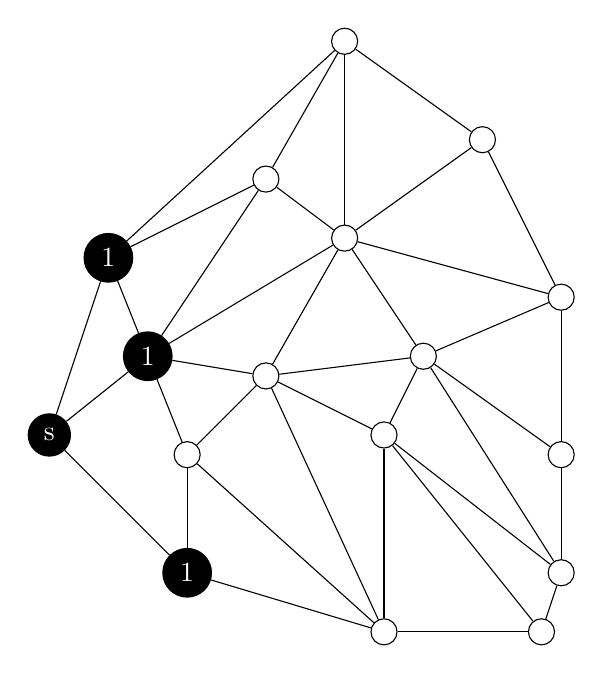
\begin{tikzpicture}
            \tikzstyle{white-fill}=[fill=white, draw=black, shape=circle]
            \tikzstyle{black-fill}=[fill=black, draw=black, shape=circle, text=white]

            \node [style=black-fill] (0) at (-2.25, -0.5) {s};
            \node [style=black-fill] (1) at (-1.5, 1.75) {1};
            \node [style=white-fill] (2) at (0.5, 0.25) {};
            \node [style=white-fill] (3) at (-0.5, -0.75) {};
            \node [style=black-fill] (4) at (-0.5, -2.25) {1};
            \node [style=black-fill] (5) at (-1, 0.5) {1};
            \node [style=white-fill] (6) at (0.5, 2.75) {};
            \node [style=white-fill] (7) at (1.5, 2) {};
            \node [style=white-fill] (8) at (2.5, 0.5) {};
            \node [style=white-fill] (9) at (2, -0.5) {};
            \node [style=white-fill] (10) at (2, -3) {};
            \node [style=white-fill] (11) at (1.5, 4.5) {};
            \node [style=white-fill] (12) at (3.25, 3.25) {};
            \node [style=white-fill] (13) at (4.25, 1.25) {};
            \node [style=white-fill] (14) at (4.25, -0.75) {};
            \node [style=white-fill] (15) at (4.25, -2.25) {};
            \node [style=white-fill] (16) at (4, -3) {};
            \draw (1) to (0);
            \draw (5) to (3);
            \draw (0) to (5);
            \draw (0) to (4);
            \draw (4) to (10);
            \draw (3) to (2);
            \draw (11) to (1);
            \draw (5) to (7);
            \draw (6) to (7);
            \draw (6) to (11);
            \draw (6) to (1);
            \draw (7) to (12);
            \draw (11) to (12);
            \draw (7) to (8);
            \draw (7) to (2);
            \draw (2) to (10);
            \draw (2) to (9);
            \draw (8) to (9);
            \draw (3) to (4);
            \draw (9) to (16);
            \draw (10) to (16);
            \draw (8) to (15);
            \draw (15) to (16);
            \draw (8) to (14);
            \draw (14) to (13);
            \draw (13) to (7);
            \draw (8) to (13);
            \draw (15) to (14);
            \draw (3) to (10);
            \draw (9) to (10);
            \draw (5) to (2);
            \draw (5) to (1);
            \draw (5) to (6);
            \draw (2) to (8);
            \draw (11) to (7);
            \draw (12) to (13);
            \draw (9) to (15);
        \end{tikzpicture}

        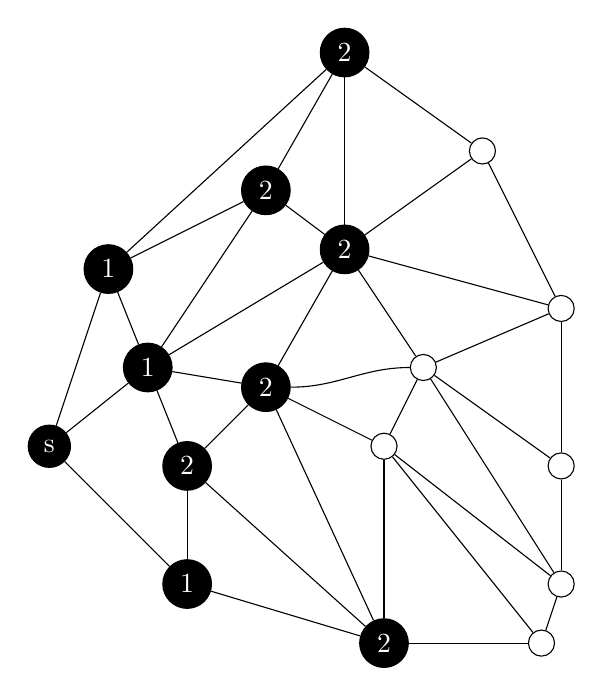
\begin{tikzpicture}
            \tikzstyle{white-fill}=[fill=white, draw=black, shape=circle]
            \tikzstyle{black-fill}=[fill=black, draw=black, shape=circle, text=white]

            \node [style=black-fill] (0) at (-2.25, -0.5) {s};
            \node [style=black-fill] (1) at (-1.5, 1.75) {1};
            \node [style=black-fill] (2) at (0.5, 0.25) {2};
            \node [style=black-fill] (3) at (-0.5, -0.75) {2};
            \node [style=black-fill] (4) at (-0.5, -2.25) {1};
            \node [style=black-fill] (5) at (-1, 0.5) {1};
            \node [style=black-fill] (6) at (0.5, 2.75) {2};
            \node [style=black-fill] (7) at (1.5, 2) {2};
            \node [style=white-fill] (8) at (2.5, 0.5) {};
            \node [style=white-fill] (9) at (2, -0.5) {};
            \node [style=black-fill] (10) at (2, -3) {2};
            \node [style=black-fill] (11) at (1.5, 4.5) {2};
            \node [style=white-fill] (12) at (3.25, 3.25) {};
            \node [style=white-fill] (13) at (4.25, 1.25) {};
            \node [style=white-fill] (14) at (4.25, -0.75) {};
            \node [style=white-fill] (15) at (4.25, -2.25) {};
            \node [style=white-fill] (16) at (4, -3) {};
            \draw (1) to (0);
            \draw (5) to (3);
            \draw (0) to (5);
            \draw (0) to (4);
            \draw (4) to (10);
            \draw (3) to (2);
            \draw (11) to (1);
            \draw (5) to (7);
            \draw (6) to (7);
            \draw (6) to (11);
            \draw (6) to (1);
            \draw (7) to (12);
            \draw (11) to (12);
            \draw (7) to (8);
            \draw (7) to (2);
            \draw (2) to (10);
            \draw (2) to (9);
            \draw (8) to (9);
            \draw (3) to (4);
            \draw (9) to (16);
            \draw (10) to (16);
            \draw (8) to (15);
            \draw (15) to (16);
            \draw (8) to (14);
            \draw (14) to (13);
            \draw (13) to (7);
            \draw (8) to (13);
            \draw (15) to (14);
            \draw (3) to (10);
            \draw (9) to (10);
            \draw (5) to (2);
            \draw (5) to (1);
            \draw (5) to (6);
            \draw [in=180, out=0] (2) to (8);
            \draw (11) to (7);
            \draw (12) to (13);
            \draw (9) to (15);
        \end{tikzpicture}

        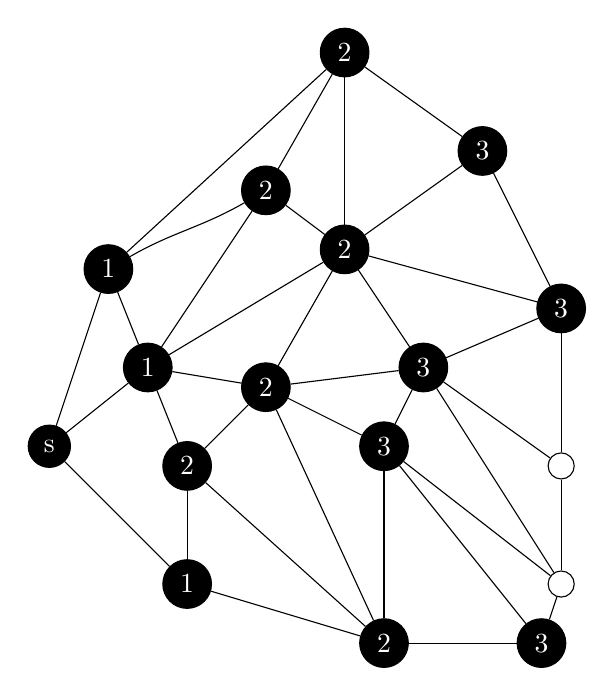
\begin{tikzpicture}
            \tikzstyle{white-fill}=[fill=white, draw=black, shape=circle]
            \tikzstyle{black-fill}=[fill=black, draw=black, shape=circle, text=white]

            \node [style=black-fill] (0) at (-2.25, -0.5) {s};
            \node [style=black-fill] (1) at (-1.5, 1.75) {1};
            \node [style=black-fill] (2) at (0.5, 0.25) {2};
            \node [style=black-fill] (3) at (-0.5, -0.75) {2};
            \node [style=black-fill] (4) at (-0.5, -2.25) {1};
            \node [style=black-fill] (5) at (-1, 0.5) {1};
            \node [style=black-fill] (6) at (0.5, 2.75) {2};
            \node [style=black-fill] (7) at (1.5, 2) {2};
            \node [style=black-fill] (8) at (2.5, 0.5) {3};
            \node [style=black-fill] (9) at (2, -0.5) {3};
            \node [style=black-fill] (10) at (2, -3) {2};
            \node [style=black-fill] (11) at (1.5, 4.5) {2};
            \node [style=black-fill] (12) at (3.25, 3.25) {3};
            \node [style=black-fill] (13) at (4.25, 1.25) {3};
            \node [style=white-fill] (14) at (4.25, -0.75) {};
            \node [style=white-fill] (15) at (4.25, -2.25) {};
            \node [style=black-fill] (16) at (4, -3) {3};
            \draw (1) to (0);
            \draw (5) to (3);
            \draw (0) to (5);
            \draw (0) to (4);
            \draw (4) to (10);
            \draw (3) to (2);
            \draw (11) to (1);
            \draw (5) to (7);
            \draw (6) to (7);
            \draw (6) to (11);
            \draw [in=30, out=-150] (6) to (1);
            \draw (7) to (12);
            \draw (11) to (12);
            \draw (7) to (8);
            \draw (7) to (2);
            \draw (2) to (10);
            \draw (2) to (9);
            \draw (8) to (9);
            \draw (3) to (4);
            \draw (9) to (16);
            \draw (10) to (16);
            \draw (8) to (15);
            \draw (15) to (16);
            \draw (8) to (14);
            \draw (14) to (13);
            \draw (13) to (7);
            \draw (8) to (13);
            \draw (15) to (14);
            \draw (3) to (10);
            \draw (9) to (10);
            \draw (5) to (2);
            \draw (5) to (1);
            \draw (5) to (6);
            \draw (2) to (8);
            \draw (11) to (7);
            \draw (12) to (13);
            \draw (9) to (15);
        \end{tikzpicture}

        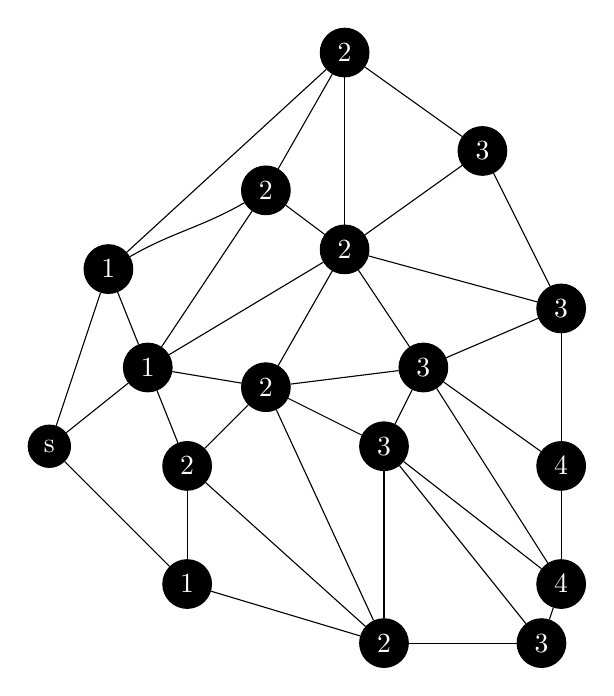
\begin{tikzpicture}
            \tikzstyle{white-fill}=[fill=white, draw=black, shape=circle]
            \tikzstyle{black-fill}=[fill=black, draw=black, shape=circle, text=white]
            \node [style=black-fill] (0) at (-2.25, -0.5) {s};
            \node [style=black-fill] (1) at (-1.5, 1.75) {1};
            \node [style=black-fill] (2) at (0.5, 0.25) {2};
            \node [style=black-fill] (3) at (-0.5, -0.75) {2};
            \node [style=black-fill] (4) at (-0.5, -2.25) {1};
            \node [style=black-fill] (5) at (-1, 0.5) {1};
            \node [style=black-fill] (6) at (0.5, 2.75) {2};
            \node [style=black-fill] (7) at (1.5, 2) {2};
            \node [style=black-fill] (8) at (2.5, 0.5) {3};
            \node [style=black-fill] (9) at (2, -0.5) {3};
            \node [style=black-fill] (10) at (2, -3) {2};
            \node [style=black-fill] (11) at (1.5, 4.5) {2};
            \node [style=black-fill] (12) at (3.25, 3.25) {3};
            \node [style=black-fill] (13) at (4.25, 1.25) {3};
            \node [style=black-fill] (14) at (4.25, -0.75) {4};
            \node [style=black-fill] (15) at (4.25, -2.25) {4};
            \node [style=black-fill] (16) at (4, -3) {3};
            \draw (1) to (0);
            \draw (5) to (3);
            \draw (0) to (5);
            \draw (0) to (4);
            \draw (4) to (10);
            \draw (3) to (2);
            \draw (11) to (1);
            \draw (5) to (7);
            \draw (6) to (7);
            \draw (6) to (11);
            \draw [in=30, out=-150] (6) to (1);
            \draw (7) to (12);
            \draw (11) to (12);
            \draw (7) to (8);
            \draw (7) to (2);
            \draw (2) to (10);
            \draw (2) to (9);
            \draw (8) to (9);
            \draw (3) to (4);
            \draw (9) to (16);
            \draw (10) to (16);
            \draw (8) to (15);
            \draw (15) to (16);
            \draw (8) to (14);
            \draw (14) to (13);
            \draw (13) to (7);
            \draw (8) to (13);
            \draw [in=270, out=90] (15) to (14);
            \draw (3) to (10);
            \draw (9) to (10);
            \draw (5) to (2);
            \draw (5) to (1);
            \draw (5) to (6);
            \draw (2) to (8);
            \draw (11) to (7);
            \draw (12) to (13);
            \draw (9) to (15);
        \end{tikzpicture}

    \end{center}

    \newpage

    \subsection{Przeszukiwanie wgłąb}
    \begin{center}

        \[P = \{\}\]

        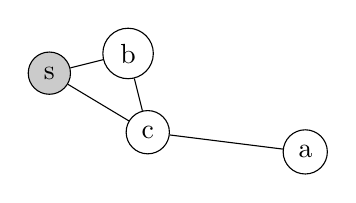
\begin{tikzpicture}
            % Node styles
            \tikzstyle{white-fill}=[fill=white, draw=black, shape=circle]
            \tikzstyle{black-fill}=[fill=black, draw=black, shape=circle, text=white]
            \tikzstyle{grey-fill}=[fill={rgb,255: red,203; green,203; blue,203}, draw=black, shape=circle]
            \node [style=grey-fill] (0) at (-1.75, -0.25) {s};
            \node [style=white-fill] (2) at (-0.75, 0) {b};
            \node [style=white-fill] (3) at (-0.5, -1) {c};
            \node [style=white-fill] (4) at (1.5, -1.25) {a};
            \draw (0) to (2);
            \draw (0) to (3);
            \draw (3) to (4);
            \draw (2) to (3);
        \end{tikzpicture}

        \[P = \{b : s\}\]

        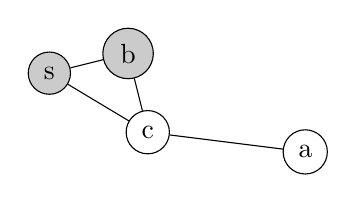
\begin{tikzpicture}
            % Node styles
            \tikzstyle{white-fill}=[fill=white, draw=black, shape=circle]
            \tikzstyle{black-fill}=[fill=black, draw=black, shape=circle, text=white]
            \tikzstyle{grey-fill}=[fill={rgb,255: red,203; green,203; blue,203}, draw=black, shape=circle]
            \node [style=grey-fill] (0) at (-1.75, -0.25) {s};
            \node [style=grey-fill] (2) at (-0.75, 0) {b};
            \node [style=white-fill] (3) at (-0.5, -1) {c};
            \node [style=white-fill] (4) at (1.5, -1.25) {a};
            \draw (0) to (2);
            \draw (0) to (3);
            \draw (3) to (4);
            \draw (2) to (3);
        \end{tikzpicture}

        \[P = \{b : s, c: b\}\]

        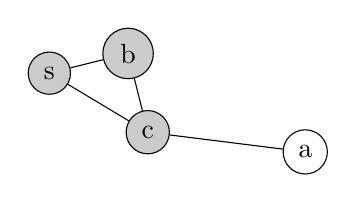
\begin{tikzpicture}
            % Node styles
            \tikzstyle{white-fill}=[fill=white, draw=black, shape=circle]
            \tikzstyle{black-fill}=[fill=black, draw=black, shape=circle, text=white]
            \tikzstyle{grey-fill}=[fill={rgb,255: red,203; green,203; blue,203}, draw=black, shape=circle]
            \node [style=grey-fill] (0) at (-1.75, -0.25) {s};
            \node [style=grey-fill] (2) at (-0.75, 0) {b};
            \node [style=grey-fill] (3) at (-0.5, -1) {c};
            \node [style=white-fill] (4) at (1.5, -1.25) {a};
            \draw (0) to (2);
            \draw (0) to (3);
            \draw (3) to (4);
            \draw (2) to (3);
        \end{tikzpicture}

        \[P = \{b : s, c : b, a : c\}\]

        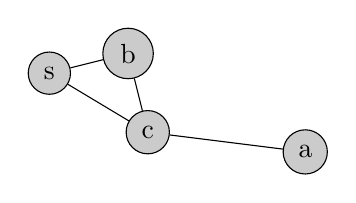
\begin{tikzpicture}
            % Node styles
            \tikzstyle{white-fill}=[fill=white, draw=black, shape=circle]
            \tikzstyle{black-fill}=[fill=black, draw=black, shape=circle, text=white]
            \tikzstyle{grey-fill}=[fill={rgb,255: red,203; green,203; blue,203}, draw=black, shape=circle]
            \node [style=grey-fill] (0) at (-1.75, -0.25) {s};
            \node [style=grey-fill] (2) at (-0.75, 0) {b};
            \node [style=grey-fill] (3) at (-0.5, -1) {c};
            \node [style=grey-fill] (4) at (1.5, -1.25) {a};
            \draw (0) to (2);
            \draw (0) to (3);
            \draw (3) to (4);
            \draw (2) to (3);
        \end{tikzpicture}

        \[P = \{b : s, c : b, a : c\}\]

        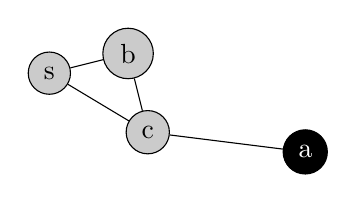
\begin{tikzpicture}
            % Node styles
            \tikzstyle{white-fill}=[fill=white, draw=black, shape=circle]
            \tikzstyle{black-fill}=[fill=black, draw=black, shape=circle, text=white]
            \tikzstyle{grey-fill}=[fill={rgb,255: red,203; green,203; blue,203}, draw=black, shape=circle]
            \node [style=grey-fill] (0) at (-1.75, -0.25) {s};
            \node [style=grey-fill] (2) at (-0.75, 0) {b};
            \node [style=grey-fill] (3) at (-0.5, -1) {c};
            \node [style=black-fill] (4) at (1.5, -1.25) {a};
            \draw (0) to (2);
            \draw (0) to (3);
            \draw (3) to (4);
            \draw (2) to (3);
        \end{tikzpicture}

        \[P = \{b : s, c : b, a : c\}\]

        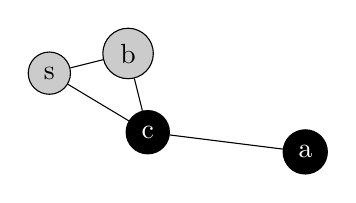
\begin{tikzpicture}
            % Node styles
            \tikzstyle{white-fill}=[fill=white, draw=black, shape=circle]
            \tikzstyle{black-fill}=[fill=black, draw=black, shape=circle, text=white]
            \tikzstyle{grey-fill}=[fill={rgb,255: red,203; green,203; blue,203}, draw=black, shape=circle]
            \node [style=grey-fill] (0) at (-1.75, -0.25) {s};
            \node [style=grey-fill] (2) at (-0.75, 0) {b};
            \node [style=black-fill] (3) at (-0.5, -1) {c};
            \node [style=black-fill] (4) at (1.5, -1.25) {a};
            \draw (0) to (2);
            \draw (0) to (3);
            \draw (3) to (4);
            \draw (2) to (3);
        \end{tikzpicture}

        \[P = \{b : s, c : b, a : c\}\]

        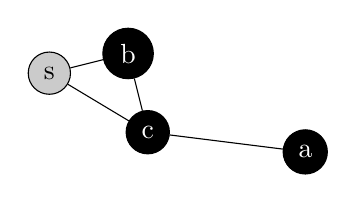
\begin{tikzpicture}
            % Node styles
            \tikzstyle{white-fill}=[fill=white, draw=black, shape=circle]
            \tikzstyle{black-fill}=[fill=black, draw=black, shape=circle, text=white]
            \tikzstyle{grey-fill}=[fill={rgb,255: red,203; green,203; blue,203}, draw=black, shape=circle]
            \node [style=grey-fill] (0) at (-1.75, -0.25) {s};
            \node [style=black-fill] (2) at (-0.75, 0) {b};
            \node [style=black-fill] (3) at (-0.5, -1) {c};
            \node [style=black-fill] (4) at (1.5, -1.25) {a};
            \draw (0) to (2);
            \draw (0) to (3);
            \draw (3) to (4);
            \draw (2) to (3);
        \end{tikzpicture}

        \[P = \{b : s, c : b, a : c\}\]

        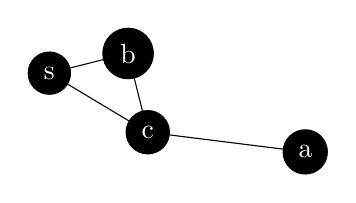
\begin{tikzpicture}
            % Node styles
            \tikzstyle{white-fill}=[fill=white, draw=black, shape=circle]
            \tikzstyle{black-fill}=[fill=black, draw=black, shape=circle, text=white]
            \tikzstyle{grey-fill}=[fill={rgb,255: red,203; green,203; blue,203}, draw=black, shape=circle]
            \node [style=black-fill] (0) at (-1.75, -0.25) {s};
            \node [style=black-fill] (2) at (-0.75, 0) {b};
            \node [style=black-fill] (3) at (-0.5, -1) {c};
            \node [style=black-fill] (4) at (1.5, -1.25) {a};
            \draw (0) to (2);
            \draw (0) to (3);
            \draw (3) to (4);
            \draw (2) to (3);
        \end{tikzpicture}
    \end{center}

    \newpage

    \subsubsection{Sortowanie topologiczne z użyciem DFS}
    \[\]
    \textbf{DAG} (\textit{directed acyclic graph}):
    graf skierowany bez cykli. Przykłady użycia: graf dziedziczenia, menadżer pakietów,
    drzewo technologii.
    \[\]
    \textbf{Problem:} Dla DAG podaj listę wierzchołków w takiej kolejności,
    aby dla każdej krawędzi $u \rightarrow v$, $u$ będzie występował przed $v$.
    \[\]
    \textbf{Algorytm:}
    \begin{enumerate}
        \item Wykonaj DFS (zaczynając od dowolnego białego wierzchołka).
        \item Przy kolorowaniu wierzchołka na czarno, przypisz mu rangę, zaczynając od 1.
        \item Powtarzaj kroki 1., 2. aż do pomalowania całego grafu.
        \item Zwróć listę wierzchołków posortowanych odwrotnie według rangi
    \end{enumerate}
    \[\]
    \textbf{Złożoność:} Taka sama jak dla DFS, tzn. $\theta(v + e)$

    \begin{center}
        \[rank = \{\}\]

        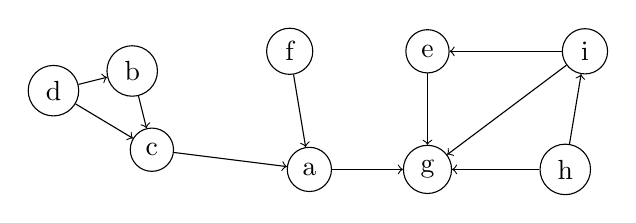
\begin{tikzpicture}
            % Node styles
            \tikzstyle{white-fill}=[fill=white, draw=black, shape=circle]
            \tikzstyle{black-fill}=[fill=black, draw=black, shape=circle, text=white]
            \tikzstyle{grey-fill}=[fill={rgb,255: red,203; green,203; blue,203}, draw=black, shape=circle]

            % Edge styles
            \tikzstyle{arrow}=[->]
            \node [style=white-fill] (0) at (-1.75, -0.25) {d};
            \node [style=white-fill] (2) at (-0.75, 0) {b};
            \node [style=white-fill] (3) at (-0.5, -1) {c};
            \node [style=white-fill] (4) at (1.5, -1.25) {a};
            \node [style=white-fill] (5) at (1.25, 0.25) {f};
            \node [style=white-fill] (6) at (3, 0.25) {e};
            \node [style=white-fill] (7) at (3, -1.25) {g};
            \node [style=white-fill] (8) at (4.75, -1.25) {h};
            \node [style=white-fill] (9) at (5, 0.25) {i};
            \draw [style=arrow] (0) to (3);
            \draw [style=arrow] (0) to (2);
            \draw [style=arrow] (2) to (3);
            \draw [style=arrow] (3) to (4);
            \draw [style=arrow] (5) to (4);
            \draw [style=arrow] (9) to (7);
            \draw [style=arrow] (8) to (9);
            \draw [style=arrow] (9) to (6);
            \draw [style=arrow] (8) to (7);
            \draw [style=arrow] (6) to (7);
            \draw [style=arrow] (4) to (7);
        \end{tikzpicture}

        \[rank = \{\}\]

        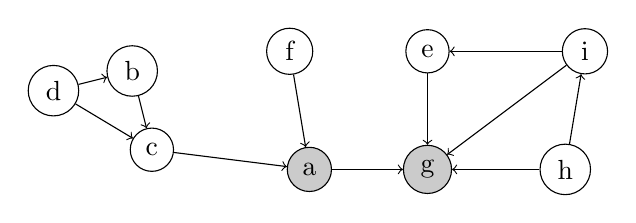
\begin{tikzpicture}
            % Node styles
            \tikzstyle{white-fill}=[fill=white, draw=black, shape=circle]
            \tikzstyle{black-fill}=[fill=black, draw=black, shape=circle, text=white]
            \tikzstyle{grey-fill}=[fill={rgb,255: red,203; green,203; blue,203}, draw=black, shape=circle]

            % Edge styles
            \tikzstyle{arrow}=[->]
            \node [style=white-fill] (0) at (-1.75, -0.25) {d};
            \node [style=white-fill] (2) at (-0.75, 0) {b};
            \node [style=white-fill] (3) at (-0.5, -1) {c};
            \node [style=grey-fill] (4) at (1.5, -1.25) {a};
            \node [style=white-fill] (5) at (1.25, 0.25) {f};
            \node [style=white-fill] (6) at (3, 0.25) {e};
            \node [style=grey-fill] (7) at (3, -1.25) {g};
            \node [style=white-fill] (8) at (4.75, -1.25) {h};
            \node [style=white-fill] (9) at (5, 0.25) {i};
            \draw [style=arrow] (0) to (3);
            \draw [style=arrow] (0) to (2);
            \draw [style=arrow] (2) to (3);
            \draw [style=arrow] (3) to (4);
            \draw [style=arrow] (5) to (4);
            \draw [style=arrow] (9) to (7);
            \draw [style=arrow] (8) to (9);
            \draw [style=arrow] (9) to (6);
            \draw [style=arrow] (8) to (7);
            \draw [style=arrow] (6) to (7);
            \draw [style=arrow] (4) to (7);
        \end{tikzpicture}

        \[rank = \{a : 2, g : 1\}\]

        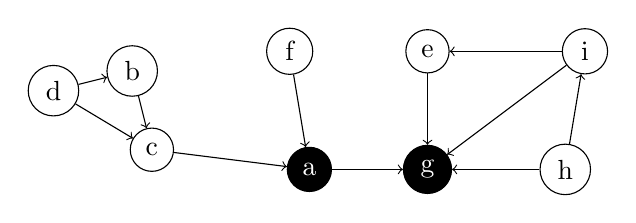
\begin{tikzpicture}
            % Node styles
            \tikzstyle{white-fill}=[fill=white, draw=black, shape=circle]
            \tikzstyle{black-fill}=[fill=black, draw=black, shape=circle, text=white]
            \tikzstyle{grey-fill}=[fill={rgb,255: red,203; green,203; blue,203}, draw=black, shape=circle]

            % Edge styles
            \tikzstyle{arrow}=[->]
            \node [style=white-fill] (0) at (-1.75, -0.25) {d};
            \node [style=white-fill] (2) at (-0.75, 0) {b};
            \node [style=white-fill] (3) at (-0.5, -1) {c};
            \node [style=black-fill] (4) at (1.5, -1.25) {a};
            \node [style=white-fill] (5) at (1.25, 0.25) {f};
            \node [style=white-fill] (6) at (3, 0.25) {e};
            \node [style=black-fill] (7) at (3, -1.25) {g};
            \node [style=white-fill] (8) at (4.75, -1.25) {h};
            \node [style=white-fill] (9) at (5, 0.25) {i};
            \draw [style=arrow] (0) to (3);
            \draw [style=arrow] (0) to (2);
            \draw [style=arrow] (2) to (3);
            \draw [style=arrow] (3) to (4);
            \draw [style=arrow] (5) to (4);
            \draw [style=arrow] (9) to (7);
            \draw [style=arrow] (8) to (9);
            \draw [style=arrow] (9) to (6);
            \draw [style=arrow] (8) to (7);
            \draw [style=arrow] (6) to (7);
            \draw [style=arrow] (4) to (7);
        \end{tikzpicture}

        \[rank = \{a : 2, g : 1\}\]

        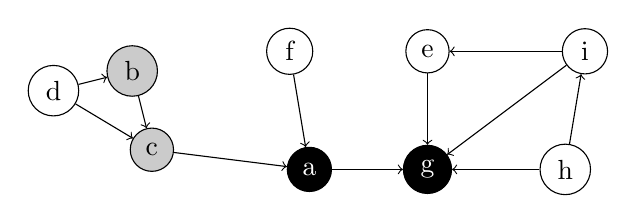
\begin{tikzpicture}
            % Node styles
            \tikzstyle{white-fill}=[fill=white, draw=black, shape=circle]
            \tikzstyle{black-fill}=[fill=black, draw=black, shape=circle, text=white]
            \tikzstyle{grey-fill}=[fill={rgb,255: red,203; green,203; blue,203}, draw=black, shape=circle]

            % Edge styles
            \tikzstyle{arrow}=[->]
            \node [style=white-fill] (0) at (-1.75, -0.25) {d};
            \node [style=grey-fill] (2) at (-0.75, 0) {b};
            \node [style=grey-fill] (3) at (-0.5, -1) {c};
            \node [style=black-fill] (4) at (1.5, -1.25) {a};
            \node [style=white-fill] (5) at (1.25, 0.25) {f};
            \node [style=white-fill] (6) at (3, 0.25) {e};
            \node [style=black-fill] (7) at (3, -1.25) {g};
            \node [style=white-fill] (8) at (4.75, -1.25) {h};
            \node [style=white-fill] (9) at (5, 0.25) {i};
            \draw [style=arrow] (0) to (3);
            \draw [style=arrow] (0) to (2);
            \draw [style=arrow] (2) to (3);
            \draw [style=arrow] (3) to (4);
            \draw [style=arrow] (5) to (4);
            \draw [style=arrow] (9) to (7);
            \draw [style=arrow] (8) to (9);
            \draw [style=arrow] (9) to (6);
            \draw [style=arrow] (8) to (7);
            \draw [style=arrow] (6) to (7);
            \draw [style=arrow] (4) to (7);
        \end{tikzpicture}

        \[rank = \{b : 4, c : 3, a : 2, g : 1\}\]

        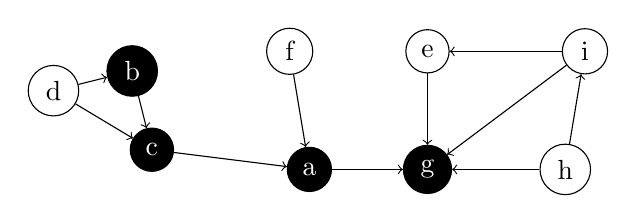
\begin{tikzpicture}
            % Node styles
            \tikzstyle{white-fill}=[fill=white, draw=black, shape=circle]
            \tikzstyle{black-fill}=[fill=black, draw=black, shape=circle, text=white]
            \tikzstyle{grey-fill}=[fill={rgb,255: red,203; green,203; blue,203}, draw=black, shape=circle]

            % Edge styles
            \tikzstyle{arrow}=[->]
            \node [style=white-fill] (0) at (-1.75, -0.25) {d};
            \node [style=black-fill] (2) at (-0.75, 0) {b};
            \node [style=black-fill] (3) at (-0.5, -1) {c};
            \node [style=black-fill] (4) at (1.5, -1.25) {a};
            \node [style=white-fill] (5) at (1.25, 0.25) {f};
            \node [style=white-fill] (6) at (3, 0.25) {e};
            \node [style=black-fill] (7) at (3, -1.25) {g};
            \node [style=white-fill] (8) at (4.75, -1.25) {h};
            \node [style=white-fill] (9) at (5, 0.25) {i};
            \draw [style=arrow] (0) to (3);
            \draw [style=arrow] (0) to (2);
            \draw [style=arrow] (2) to (3);
            \draw [style=arrow] (3) to (4);
            \draw [style=arrow] (5) to (4);
            \draw [style=arrow] (9) to (7);
            \draw [style=arrow] (8) to (9);
            \draw [style=arrow] (9) to (6);
            \draw [style=arrow] (8) to (7);
            \draw [style=arrow] (6) to (7);
            \draw [style=arrow] (4) to (7);
        \end{tikzpicture}

        \[rank = \{b : 4, c : 3, a : 2, g : 1\}\]

        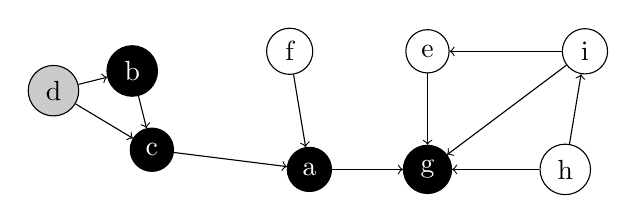
\begin{tikzpicture}
            % Node styles
            \tikzstyle{white-fill}=[fill=white, draw=black, shape=circle]
            \tikzstyle{black-fill}=[fill=black, draw=black, shape=circle, text=white]
            \tikzstyle{grey-fill}=[fill={rgb,255: red,203; green,203; blue,203}, draw=black, shape=circle]

            % Edge styles
            \tikzstyle{arrow}=[->]
            \node [style=grey-fill] (0) at (-1.75, -0.25) {d};
            \node [style=black-fill] (2) at (-0.75, 0) {b};
            \node [style=black-fill] (3) at (-0.5, -1) {c};
            \node [style=black-fill] (4) at (1.5, -1.25) {a};
            \node [style=white-fill] (5) at (1.25, 0.25) {f};
            \node [style=white-fill] (6) at (3, 0.25) {e};
            \node [style=black-fill] (7) at (3, -1.25) {g};
            \node [style=white-fill] (8) at (4.75, -1.25) {h};
            \node [style=white-fill] (9) at (5, 0.25) {i};
            \draw [style=arrow] (0) to (3);
            \draw [style=arrow] (0) to (2);
            \draw [style=arrow] (2) to (3);
            \draw [style=arrow] (3) to (4);
            \draw [style=arrow] (5) to (4);
            \draw [style=arrow] (9) to (7);
            \draw [style=arrow] (8) to (9);
            \draw [style=arrow] (9) to (6);
            \draw [style=arrow] (8) to (7);
            \draw [style=arrow] (6) to (7);
            \draw [style=arrow] (4) to (7);
        \end{tikzpicture}

        \[rank = \{d : 5, b : 4, c : 3, a : 2, g : 1\}\]

        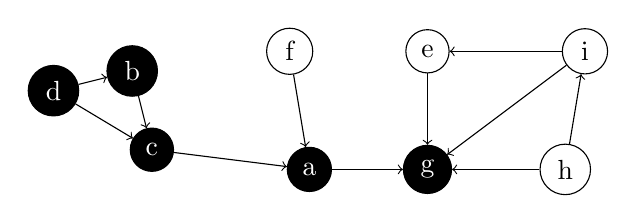
\begin{tikzpicture}
            % Node styles
            \tikzstyle{white-fill}=[fill=white, draw=black, shape=circle]
            \tikzstyle{black-fill}=[fill=black, draw=black, shape=circle, text=white]
            \tikzstyle{grey-fill}=[fill={rgb,255: red,203; green,203; blue,203}, draw=black, shape=circle]

            % Edge styles
            \tikzstyle{arrow}=[->]
            \node [style=black-fill] (0) at (-1.75, -0.25) {d};
            \node [style=black-fill] (2) at (-0.75, 0) {b};
            \node [style=black-fill] (3) at (-0.5, -1) {c};
            \node [style=black-fill] (4) at (1.5, -1.25) {a};
            \node [style=white-fill] (5) at (1.25, 0.25) {f};
            \node [style=white-fill] (6) at (3, 0.25) {e};
            \node [style=black-fill] (7) at (3, -1.25) {g};
            \node [style=white-fill] (8) at (4.75, -1.25) {h};
            \node [style=white-fill] (9) at (5, 0.25) {i};
            \draw [style=arrow] (0) to (3);
            \draw [style=arrow] (0) to (2);
            \draw [style=arrow] (2) to (3);
            \draw [style=arrow] (3) to (4);
            \draw [style=arrow] (5) to (4);
            \draw [style=arrow] (9) to (7);
            \draw [style=arrow] (8) to (9);
            \draw [style=arrow] (9) to (6);
            \draw [style=arrow] (8) to (7);
            \draw [style=arrow] (6) to (7);
            \draw [style=arrow] (4) to (7);
        \end{tikzpicture}

        \[rank = \{d : 5, b : 4, c : 3, a : 2, g : 1\}\]

        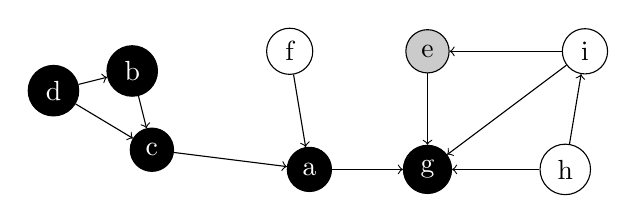
\begin{tikzpicture}
            % Node styles
            \tikzstyle{white-fill}=[fill=white, draw=black, shape=circle]
            \tikzstyle{black-fill}=[fill=black, draw=black, shape=circle, text=white]
            \tikzstyle{grey-fill}=[fill={rgb,255: red,203; green,203; blue,203}, draw=black, shape=circle]

            % Edge styles
            \tikzstyle{arrow}=[->]
            \node [style=black-fill] (0) at (-1.75, -0.25) {d};
            \node [style=black-fill] (2) at (-0.75, 0) {b};
            \node [style=black-fill] (3) at (-0.5, -1) {c};
            \node [style=black-fill] (4) at (1.5, -1.25) {a};
            \node [style=white-fill] (5) at (1.25, 0.25) {f};
            \node [style=grey-fill] (6) at (3, 0.25) {e};
            \node [style=black-fill] (7) at (3, -1.25) {g};
            \node [style=white-fill] (8) at (4.75, -1.25) {h};
            \node [style=white-fill] (9) at (5, 0.25) {i};
            \draw [style=arrow] (0) to (3);
            \draw [style=arrow] (0) to (2);
            \draw [style=arrow] (2) to (3);
            \draw [style=arrow] (3) to (4);
            \draw [style=arrow] (5) to (4);
            \draw [style=arrow] (9) to (7);
            \draw [style=arrow] (8) to (9);
            \draw [style=arrow] (9) to (6);
            \draw [style=arrow] (8) to (7);
            \draw [style=arrow] (6) to (7);
            \draw [style=arrow] (4) to (7);
        \end{tikzpicture}

        \[rank = \{e : 6, d : 5, b : 4, c : 3, a : 2, g : 1\}\]

        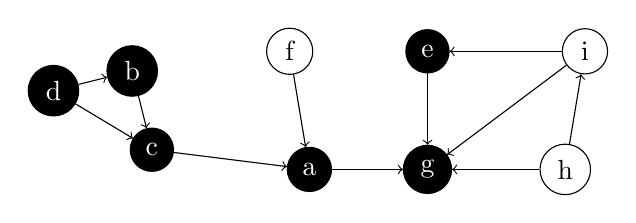
\begin{tikzpicture}
            % Node styles
            \tikzstyle{white-fill}=[fill=white, draw=black, shape=circle]
            \tikzstyle{black-fill}=[fill=black, draw=black, shape=circle, text=white]
            \tikzstyle{grey-fill}=[fill={rgb,255: red,203; green,203; blue,203}, draw=black, shape=circle]

            % Edge styles
            \tikzstyle{arrow}=[->]
            \node [style=black-fill] (0) at (-1.75, -0.25) {d};
            \node [style=black-fill] (2) at (-0.75, 0) {b};
            \node [style=black-fill] (3) at (-0.5, -1) {c};
            \node [style=black-fill] (4) at (1.5, -1.25) {a};
            \node [style=white-fill] (5) at (1.25, 0.25) {f};
            \node [style=black-fill] (6) at (3, 0.25) {e};
            \node [style=black-fill] (7) at (3, -1.25) {g};
            \node [style=white-fill] (8) at (4.75, -1.25) {h};
            \node [style=white-fill] (9) at (5, 0.25) {i};
            \draw [style=arrow] (0) to (3);
            \draw [style=arrow] (0) to (2);
            \draw [style=arrow] (2) to (3);
            \draw [style=arrow] (3) to (4);
            \draw [style=arrow] (5) to (4);
            \draw [style=arrow] (9) to (7);
            \draw [style=arrow] (8) to (9);
            \draw [style=arrow] (9) to (6);
            \draw [style=arrow] (8) to (7);
            \draw [style=arrow] (6) to (7);
            \draw [style=arrow] (4) to (7);
        \end{tikzpicture}

        \[rank = \{e : 6, d : 5, b : 4, c : 3, a : 2, g : 1\}\]

        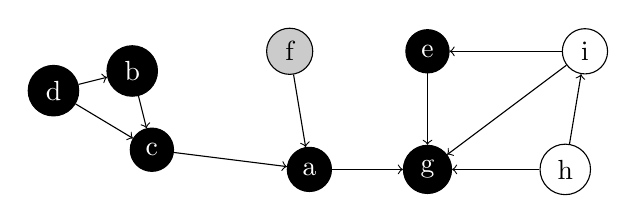
\begin{tikzpicture}
            % Node styles
            \tikzstyle{white-fill}=[fill=white, draw=black, shape=circle]
            \tikzstyle{black-fill}=[fill=black, draw=black, shape=circle, text=white]
            \tikzstyle{grey-fill}=[fill={rgb,255: red,203; green,203; blue,203}, draw=black, shape=circle]

            % Edge styles
            \tikzstyle{arrow}=[->]
            \node [style=black-fill] (0) at (-1.75, -0.25) {d};
            \node [style=black-fill] (2) at (-0.75, 0) {b};
            \node [style=black-fill] (3) at (-0.5, -1) {c};
            \node [style=black-fill] (4) at (1.5, -1.25) {a};
            \node [style=grey-fill] (5) at (1.25, 0.25) {f};
            \node [style=black-fill] (6) at (3, 0.25) {e};
            \node [style=black-fill] (7) at (3, -1.25) {g};
            \node [style=white-fill] (8) at (4.75, -1.25) {h};
            \node [style=white-fill] (9) at (5, 0.25) {i};
            \draw [style=arrow] (0) to (3);
            \draw [style=arrow] (0) to (2);
            \draw [style=arrow] (2) to (3);
            \draw [style=arrow] (3) to (4);
            \draw [style=arrow] (5) to (4);
            \draw [style=arrow] (9) to (7);
            \draw [style=arrow] (8) to (9);
            \draw [style=arrow] (9) to (6);
            \draw [style=arrow] (8) to (7);
            \draw [style=arrow] (6) to (7);
            \draw [style=arrow] (4) to (7);
        \end{tikzpicture}

        \[rank = \{f : 7, e : 6, d : 5, b : 4, c : 3, a : 2, g : 1\}\]

        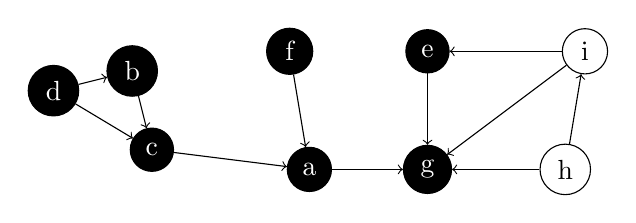
\begin{tikzpicture}
            % Node styles
            \tikzstyle{white-fill}=[fill=white, draw=black, shape=circle]
            \tikzstyle{black-fill}=[fill=black, draw=black, shape=circle, text=white]
            \tikzstyle{grey-fill}=[fill={rgb,255: red,203; green,203; blue,203}, draw=black, shape=circle]

            % Edge styles
            \tikzstyle{arrow}=[->]
            \node [style=black-fill] (0) at (-1.75, -0.25) {d};
            \node [style=black-fill] (2) at (-0.75, 0) {b};
            \node [style=black-fill] (3) at (-0.5, -1) {c};
            \node [style=black-fill] (4) at (1.5, -1.25) {a};
            \node [style=black-fill] (5) at (1.25, 0.25) {f};
            \node [style=black-fill] (6) at (3, 0.25) {e};
            \node [style=black-fill] (7) at (3, -1.25) {g};
            \node [style=white-fill] (8) at (4.75, -1.25) {h};
            \node [style=white-fill] (9) at (5, 0.25) {i};
            \draw [style=arrow] (0) to (3);
            \draw [style=arrow] (0) to (2);
            \draw [style=arrow] (2) to (3);
            \draw [style=arrow] (3) to (4);
            \draw [style=arrow] (5) to (4);
            \draw [style=arrow] (9) to (7);
            \draw [style=arrow] (8) to (9);
            \draw [style=arrow] (9) to (6);
            \draw [style=arrow] (8) to (7);
            \draw [style=arrow] (6) to (7);
            \draw [style=arrow] (4) to (7);
        \end{tikzpicture}

        \[rank = \{f : 7, e : 6, d : 5, b : 4, c : 3, a : 2, g : 1\}\]

        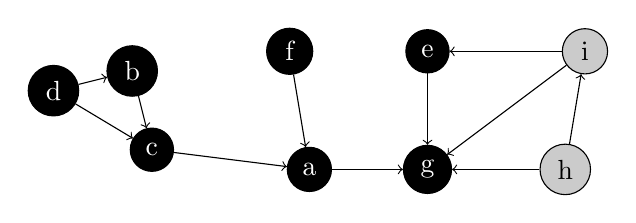
\begin{tikzpicture}
            % Node styles
            \tikzstyle{white-fill}=[fill=white, draw=black, shape=circle]
            \tikzstyle{black-fill}=[fill=black, draw=black, shape=circle, text=white]
            \tikzstyle{grey-fill}=[fill={rgb,255: red,203; green,203; blue,203}, draw=black, shape=circle]

            % Edge styles
            \tikzstyle{arrow}=[->]
            \node [style=black-fill] (0) at (-1.75, -0.25) {d};
            \node [style=black-fill] (2) at (-0.75, 0) {b};
            \node [style=black-fill] (3) at (-0.5, -1) {c};
            \node [style=black-fill] (4) at (1.5, -1.25) {a};
            \node [style=black-fill] (5) at (1.25, 0.25) {f};
            \node [style=black-fill] (6) at (3, 0.25) {e};
            \node [style=black-fill] (7) at (3, -1.25) {g};
            \node [style=grey-fill] (8) at (4.75, -1.25) {h};
            \node [style=grey-fill] (9) at (5, 0.25) {i};
            \draw [style=arrow] (0) to (3);
            \draw [style=arrow] (0) to (2);
            \draw [style=arrow] (2) to (3);
            \draw [style=arrow] (3) to (4);
            \draw [style=arrow] (5) to (4);
            \draw [style=arrow] (9) to (7);
            \draw [style=arrow] (8) to (9);
            \draw [style=arrow] (9) to (6);
            \draw [style=arrow] (8) to (7);
            \draw [style=arrow] (6) to (7);
            \draw [style=arrow] (4) to (7);
        \end{tikzpicture}

        \[rank = \{h : 9, i : 8, f : 7, e : 6, d : 5, b : 4, c : 3, a : 2, g : 1\}\]

        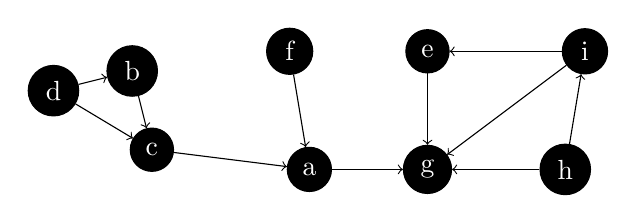
\begin{tikzpicture}
            % Node styles
            \tikzstyle{white-fill}=[fill=white, draw=black, shape=circle]
            \tikzstyle{black-fill}=[fill=black, draw=black, shape=circle, text=white]
            \tikzstyle{grey-fill}=[fill={rgb,255: red,203; green,203; blue,203}, draw=black, shape=circle]

            % Edge styles
            \tikzstyle{arrow}=[->]
            \node [style=black-fill] (0) at (-1.75, -0.25) {d};
            \node [style=black-fill] (2) at (-0.75, 0) {b};
            \node [style=black-fill] (3) at (-0.5, -1) {c};
            \node [style=black-fill] (4) at (1.5, -1.25) {a};
            \node [style=black-fill] (5) at (1.25, 0.25) {f};
            \node [style=black-fill] (6) at (3, 0.25) {e};
            \node [style=black-fill] (7) at (3, -1.25) {g};
            \node [style=black-fill] (8) at (4.75, -1.25) {h};
            \node [style=black-fill] (9) at (5, 0.25) {i};
            \draw [style=arrow] (0) to (3);
            \draw [style=arrow] (0) to (2);
            \draw [style=arrow] (2) to (3);
            \draw [style=arrow] (3) to (4);
            \draw [style=arrow] (5) to (4);
            \draw [style=arrow] (9) to (7);
            \draw [style=arrow] (8) to (9);
            \draw [style=arrow] (9) to (6);
            \draw [style=arrow] (8) to (7);
            \draw [style=arrow] (6) to (7);
            \draw [style=arrow] (4) to (7);
        \end{tikzpicture}

        \[result = [h, i, f, e, d, b, c, a, g]\]
    \end{center}

    \newpage

    \section{Algorytmy wyszukiwania najkrótszej ścieżki (Dijkstry oraz Bellmana-Forda).}

    \subsection{Algorytm Dijkstry}

    \begin{center}

        \begin{gather*}
            D = \{s : 0, a : \infty, b : \infty, c : \infty, d : \infty\}\\
            P = \{\}\\
        \end{gather*}

        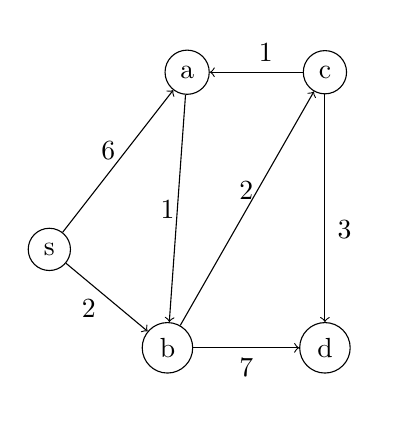
\begin{tikzpicture}
            % Node styles
            \tikzstyle{white-fill}=[fill=white, draw=black, shape=circle]
            \tikzstyle{invisible}=[fill=white, draw=white, shape=circle]
            \tikzstyle{black-fill}=[fill=black, draw=black, shape=circle, text=white]

            % Edge styles
            \tikzstyle{arrow}=[->]
            \node [style=white-fill] (0) at (-3, 0) {s};
            \node [style=white-fill] (1) at (-1.25, 2.25) {};
            \node [style=white-fill] (2) at (-1.5, -1.25) {b};
            \node [style=white-fill] (3) at (0.5, 2.25) {c};
            \node [style=white-fill] (4) at (0.5, -1.25) {d};
            \node [style=white-fill] (5) at (-1.25, 2.25) {a};
            \node [style=invisible] (6) at (-2.25, 1.25) {6};
            \node [style=invisible] (7) at (-2.5, -0.75) {2};
            \node [style=invisible] (8) at (-1.5, 0.5) {1};
            \node [style=invisible] (9) at (-0.25, 2.5) {1};
            \node [style=invisible] (10) at (-0.5, 0.75) {2};
            \node [style=invisible] (11) at (-0.5, -1.5) {7};
            \node [style=invisible] (12) at (0.75, 0.25) {3};
            \draw [style=arrow] (0) to (5);
            \draw [style=arrow] (5) to (2);
            \draw [style=arrow] (0) to (2);
            \draw [style=arrow] (2) to (4);
            \draw [style=arrow] (3) to (4);
            \draw [style=arrow] (2) to (3);
            \draw [style=arrow] (3) to (5);
        \end{tikzpicture}

        \begin{gather*}
            D = \{s : 0, \mathbf{a : 6, b : 2}, c : \infty, d : \infty\}\\
            P = \{\mathbf{a : s, b : s}\}\\
        \end{gather*}

        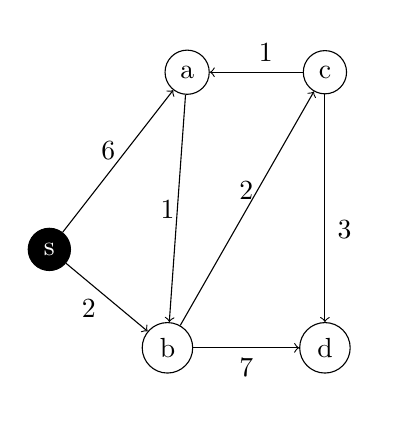
\begin{tikzpicture}
            % Node styles
            \tikzstyle{white-fill}=[fill=white, draw=black, shape=circle]
            \tikzstyle{invisible}=[fill=white, draw=white, shape=circle]
            \tikzstyle{black-fill}=[fill=black, draw=black, shape=circle, text=white]

            % Edge styles
            \tikzstyle{arrow}=[->]
            \node [style=black-fill] (0) at (-3, 0) {s};
            \node [style=white-fill] (1) at (-1.25, 2.25) {};
            \node [style=white-fill] (2) at (-1.5, -1.25) {b};
            \node [style=white-fill] (3) at (0.5, 2.25) {c};
            \node [style=white-fill] (4) at (0.5, -1.25) {d};
            \node [style=white-fill] (5) at (-1.25, 2.25) {a};
            \node [style=invisible] (6) at (-2.25, 1.25) {6};
            \node [style=invisible] (7) at (-2.5, -0.75) {2};
            \node [style=invisible] (8) at (-1.5, 0.5) {1};
            \node [style=invisible] (9) at (-0.25, 2.5) {1};
            \node [style=invisible] (10) at (-0.5, 0.75) {2};
            \node [style=invisible] (11) at (-0.5, -1.5) {7};
            \node [style=invisible] (12) at (0.75, 0.25) {3};
            \draw [style=arrow] (0) to (5);
            \draw [style=arrow] (5) to (2);
            \draw [style=arrow] (0) to (2);
            \draw [style=arrow] (2) to (4);
            \draw [style=arrow] (3) to (4);
            \draw [style=arrow] (2) to (3);
            \draw [style=arrow] (3) to (5);
        \end{tikzpicture}

        \begin{gather*}
            D = \{s : 0, a : 6, b : 2, \mathbf{c : 4, d : 9}\}\\
            P = \{a : s, b : s, \mathbf{c : b, d : b}\}\\
        \end{gather*}

        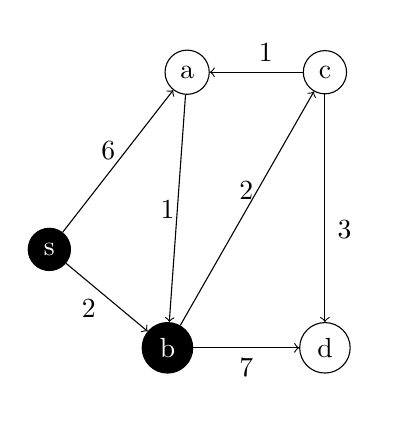
\begin{tikzpicture}
            % Node styles
            \tikzstyle{white-fill}=[fill=white, draw=black, shape=circle]
            \tikzstyle{invisible}=[fill=white, draw=white, shape=circle]
            \tikzstyle{black-fill}=[fill=black, draw=black, shape=circle, text=white]

            % Edge styles
            \tikzstyle{arrow}=[->]
            \node [style=black-fill] (0) at (-3, 0) {s};
            \node [style=white-fill] (1) at (-1.25, 2.25) {};
            \node [style=black-fill] (2) at (-1.5, -1.25) {b};
            \node [style=white-fill] (3) at (0.5, 2.25) {c};
            \node [style=white-fill] (4) at (0.5, -1.25) {d};
            \node [style=white-fill] (5) at (-1.25, 2.25) {a};
            \node [style=invisible] (6) at (-2.25, 1.25) {6};
            \node [style=invisible] (7) at (-2.5, -0.75) {2};
            \node [style=invisible] (8) at (-1.5, 0.5) {1};
            \node [style=invisible] (9) at (-0.25, 2.5) {1};
            \node [style=invisible] (10) at (-0.5, 0.75) {2};
            \node [style=invisible] (11) at (-0.5, -1.5) {7};
            \node [style=invisible] (12) at (0.75, 0.25) {3};
            \draw [style=arrow] (0) to (5);
            \draw [style=arrow] (5) to (2);
            \draw [style=arrow] (0) to (2);
            \draw [style=arrow] (2) to (4);
            \draw [style=arrow] (3) to (4);
            \draw [style=arrow] (2) to (3);
            \draw [style=arrow] (3) to (5);
        \end{tikzpicture}

        \begin{gather*}
            D = \{s : 0, \mathbf{a : 5}, b : 2, c : 4, \mathbf{d : 7}\}\\
            P = \{\mathbf{a : c}, b : s, c : b, \mathbf{d : c}\}\\
        \end{gather*}

        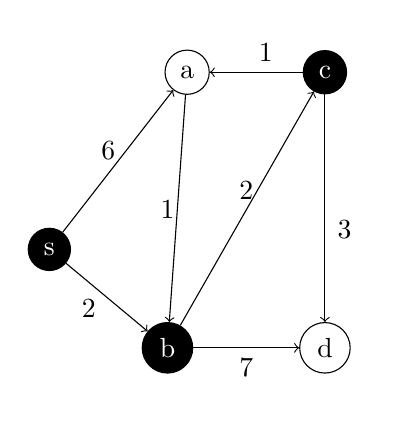
\begin{tikzpicture}
            % Node styles
            \tikzstyle{white-fill}=[fill=white, draw=black, shape=circle]
            \tikzstyle{invisible}=[fill=white, draw=white, shape=circle]
            \tikzstyle{black-fill}=[fill=black, draw=black, shape=circle, text=white]

            % Edge styles
            \tikzstyle{arrow}=[->]
            \node [style=black-fill] (0) at (-3, 0) {s};
            \node [style=white-fill] (1) at (-1.25, 2.25) {};
            \node [style=black-fill] (2) at (-1.5, -1.25) {b};
            \node [style=black-fill] (3) at (0.5, 2.25) {c};
            \node [style=white-fill] (4) at (0.5, -1.25) {d};
            \node [style=white-fill] (5) at (-1.25, 2.25) {a};
            \node [style=invisible] (6) at (-2.25, 1.25) {6};
            \node [style=invisible] (7) at (-2.5, -0.75) {2};
            \node [style=invisible] (8) at (-1.5, 0.5) {1};
            \node [style=invisible] (9) at (-0.25, 2.5) {1};
            \node [style=invisible] (10) at (-0.5, 0.75) {2};
            \node [style=invisible] (11) at (-0.5, -1.5) {7};
            \node [style=invisible] (12) at (0.75, 0.25) {3};
            \draw [style=arrow] (0) to (5);
            \draw [style=arrow] (5) to (2);
            \draw [style=arrow] (0) to (2);
            \draw [style=arrow] (2) to (4);
            \draw [style=arrow] (3) to (4);
            \draw [style=arrow] (2) to (3);
            \draw [style=arrow] (3) to (5);
        \end{tikzpicture}

        \begin{gather*}
            D = \{s : 0, a : 5, b : 2, c : 4, d : 7\}\\
            P = \{a : c, b : s, c : b, d : c\}\\
        \end{gather*}

        \begin{tikzpicture}
            % Node styles
            \tikzstyle{white-fill}=[fill=white, draw=black, shape=circle]
            \tikzstyle{invisible}=[fill=white, draw=white, shape=circle]
            \tikzstyle{black-fill}=[fill=black, draw=black, shape=circle, text=white]

            % Edge styles
            \tikzstyle{arrow}=[->]
            \node [style=black-fill] (0) at (-3, 0) {s};
            \node [style=white-fill] (1) at (-1.25, 2.25) {};
            \node [style=black-fill] (2) at (-1.5, -1.25) {b};
            \node [style=black-fill] (3) at (0.5, 2.25) {c};
            \node [style=white-fill] (4) at (0.5, -1.25) {d};
            \node [style=black-fill] (5) at (-1.25, 2.25) {a};
            \node [style=invisible] (6) at (-2.25, 1.25) {6};
            \node [style=invisible] (7) at (-2.5, -0.75) {2};
            \node [style=invisible] (8) at (-1.5, 0.5) {1};
            \node [style=invisible] (9) at (-0.25, 2.5) {1};
            \node [style=invisible] (10) at (-0.5, 0.75) {2};
            \node [style=invisible] (11) at (-0.5, -1.5) {7};
            \node [style=invisible] (12) at (0.75, 0.25) {3};
            \draw [style=arrow] (0) to (5);
            \draw [style=arrow] (5) to (2);
            \draw [style=arrow] (0) to (2);
            \draw [style=arrow] (2) to (4);
            \draw [style=arrow] (3) to (4);
            \draw [style=arrow] (2) to (3);
            \draw [style=arrow] (3) to (5);
        \end{tikzpicture}

        \begin{gather*}
            D = \{s : 0, a : 5, b : 2, c : 4, d : 7\}\\
            P = \{a : c, b : s, c : b, d : c\}\\
        \end{gather*}

        \begin{tikzpicture}
            % Node styles
            \tikzstyle{white-fill}=[fill=white, draw=black, shape=circle]
            \tikzstyle{invisible}=[fill=white, draw=white, shape=circle]
            \tikzstyle{black-fill}=[fill=black, draw=black, shape=circle, text=white]

            % Edge styles
            \tikzstyle{arrow}=[->]
            \node [style=black-fill] (0) at (-3, 0) {s};
            \node [style=white-fill] (1) at (-1.25, 2.25) {};
            \node [style=black-fill] (2) at (-1.5, -1.25) {b};
            \node [style=black-fill] (3) at (0.5, 2.25) {c};
            \node [style=black-fill] (4) at (0.5, -1.25) {d};
            \node [style=black-fill] (5) at (-1.25, 2.25) {a};
            \node [style=invisible] (6) at (-2.25, 1.25) {6};
            \node [style=invisible] (7) at (-2.5, -0.75) {2};
            \node [style=invisible] (8) at (-1.5, 0.5) {1};
            \node [style=invisible] (9) at (-0.25, 2.5) {1};
            \node [style=invisible] (10) at (-0.5, 0.75) {2};
            \node [style=invisible] (11) at (-0.5, -1.5) {7};
            \node [style=invisible] (12) at (0.75, 0.25) {3};
            \draw [style=arrow] (0) to (5);
            \draw [style=arrow] (5) to (2);
            \draw [style=arrow] (0) to (2);
            \draw [style=arrow] (2) to (4);
            \draw [style=arrow] (3) to (4);
            \draw [style=arrow] (2) to (3);
            \draw [style=arrow] (3) to (5);
        \end{tikzpicture}

    \end{center}

    \newpage

    \subsection{Algorytm Bellmana-Forda}

    \begin{center}
        \begin{tikzpicture}
            % Node styles
            \tikzstyle{white-fill}=[fill=white, draw=black, shape=circle]
            \tikzstyle{invisible}=[fill=white, draw=white, shape=circle]
            \tikzstyle{black-fill}=[fill=black, draw=black, shape=circle, text=white]

            % Edge styles
            \tikzstyle{arrow}=[->]
            \node [style=white-fill] (0) at (-3, 0) {s};
            \node [style=white-fill] (1) at (-1.25, 2.25) {};
            \node [style=white-fill] (2) at (-1.5, -1.25) {b};
            \node [style=white-fill] (3) at (0.5, 2.25) {c};
            \node [style=white-fill] (4) at (0.5, -1.25) {d};
            \node [style=white-fill] (5) at (-1.25, 2.25) {a};
            \node [style=invisible] (6) at (-2.25, 1.25) {6};
            \node [style=invisible] (7) at (-2.5, -0.75) {3};
            \node [style=invisible] (8) at (-1.75, 0.5) {-1};
            \node [style=invisible] (9) at (-0.25, 2.5) {1};
            \node [style=invisible] (10) at (-0.5, 0.75) {1};
            \node [style=invisible] (11) at (-0.5, -1.5) {-1};
            \node [style=invisible] (12) at (0.75, 0.25) {-1};
            \draw [style=arrow] (0) to (5);
            \draw [style=arrow] (5) to (2);
            \draw [style=arrow] (0) to (2);
            \draw [style=arrow] (2) to (4);
            \draw [style=arrow] (3) to (4);
            \draw [style=arrow] (2) to (3);
            \draw [style=arrow] (3) to (5);
        \end{tikzpicture}

        Wartości w $D$ w zależności od iteracji:

        \begin{tabular}{c||c|c|c|c}
            i & a & b & c & d \\
            \hline \hline
            0 & $\infty$ & $\infty$ & $\infty$ & $\infty$ \\
            \hline
            1 & 6 & 3 & $\infty$ & $\infty$ \\
            \hline
            2 & 5 & 3 & 4 & 2 \\
            \hline
            3 & 5 & 3 & 4 & 2 \\
        \end{tabular}

        Wartości w $P$ w zależności od iteracji:

        \begin{tabular}{c||c|c|c|c}
            i & a & b & c & d \\
            \hline \hline
            0 & & & &  \\
            \hline
            1 & s & s & &  \\
            \hline
            2 & c & s & b & b \\
            \hline
            3 & c & s & b & b \\
        \end{tabular}
    \end{center}

    \newpage


    \section{Programowanie dynamiczne: podział na podproblemy, porównanie z metodą "dziel i zwyciężaj".}
    \section{Algorytm zachłanny: przykład optymalnego i nieoptymalnego wykorzystania.}
    \section{Kolorowania wierzchołkowe (grafów planarnych) i krawędziowe grafów, algorytmy i ich złożoności.}

    \newpage

    \section{Algorytmy wyszukiwania minimalnego drzewa rozpinającego: Boruvki, Prima i Kruskala.}

    \begin{center}
        \begin{tikzpicture}[scale=0.15]
            \tikzstyle{every node}+=[inner sep=0pt]
            \draw [black] (17.6,-15.2) circle (3);
            \draw (17.6,-15.2) node {$1$};
            \draw [black] (39.6,-14.4) circle (3);
            \draw (39.6,-14.4) node {$2$};
            \draw [black] (59.1,-14.4) circle (3);
            \draw (59.1,-14.4) node {$3$};
            \draw [black] (72.3,-29.9) circle (3);
            \draw (72.3,-29.9) node {$4$};
            \draw [black] (59,-45.9) circle (3);
            \draw (59,-45.9) node {$5$};
            \draw [black] (40,-45.2) circle (3);
            \draw (40,-45.2) node {$6$};
            \draw [black] (17.1,-45.5) circle (3);
            \draw (17.1,-45.5) node {$7$};
            \draw [black] (6.8,-29.9) circle (3);
            \draw (6.8,-29.9) node {$0$};
            \draw [black] (39.6,-29.1) circle (3);
            \draw (39.6,-29.1) node {$8$};
            \draw [black] (8.58,-27.48) -- (15.82,-17.62);
            \draw (12.78,-23.94) node [right] {$4$};
            \draw [black] (20.6,-15.09) -- (36.6,-14.51);
            \draw (28.63,-15.34) node [below] {$8$};
            \draw [black] (42.6,-14.4) -- (56.1,-14.4);
            \draw (49.35,-14.9) node [below] {$7$};
            \draw [black] (61.05,-16.68) -- (70.35,-27.62);
            \draw (65.15,-23.59) node [left] {$9$};
            \draw [black] (70.38,-32.21) -- (60.92,-43.59);
            \draw (65.1,-36.46) node [left] {$10$};
            \draw [black] (56,-45.79) -- (43,-45.31);
            \draw (49.53,-45.01) node [above] {$2$};
            \draw [black] (37,-45.24) -- (20.1,-45.46);
            \draw (28.55,-44.84) node [above] {$1$};
            \draw [black] (15.45,-43) -- (8.45,-32.4);
            \draw (12.56,-36.37) node [right] {$8$};
            \draw [black] (17.55,-18.2) -- (17.15,-42.5);
            \draw (16.83,-30.35) node [left] {$11$};
            \draw [black] (19.52,-43.73) -- (37.18,-30.87);
            \draw (29.35,-37.8) node [below] {$7$};
            \draw [black] (39.67,-32.1) -- (39.93,-42.2);
            \draw (39.26,-37.16) node [left] {$6$};
            \draw [black] (39.6,-26.1) -- (39.6,-17.4);
            \draw (40.1,-21.75) node [right] {$2$};
            \draw [black] (41.17,-16.95) -- (57.43,-43.35);
            \draw (48.67,-31.43) node [left] {$4$};
            \draw [black] (59.01,-42.9) -- (59.09,-17.4);
            \draw (59.55,-30.15) node [right] {$14$};
        \end{tikzpicture}
    \end{center}

    \subsection{Algorytm Boruvki}
    \begin{enumerate}
        \item Wybrane krawędzie o najmniejszych wagach

        \begin{center}
            \begin{tikzpicture}[scale=0.1]
                \tikzstyle{every node}+=[inner sep=0pt]
                \draw [black] (22.8,-48.8) circle (3);
                \draw (22.8,-48.8) node {$7$};
                \draw [black] (39.7,-48.8) circle (3);
                \draw (39.7,-48.8) node {$6$};
                \draw [black] (39.7,-34.1) circle (3);
                \draw (39.7,-34.1) node {$8$};
                \draw [black] (39.7,-18.4) circle (3);
                \draw (39.7,-18.4) node {$2$};
                \draw [black] (57.3,-48.8) circle (3);
                \draw (57.3,-48.8) node {$5$};
                \draw [black] (22.8,-18.4) circle (3);
                \draw (22.8,-18.4) node {$1$};
                \draw [black] (11.5,-34.1) circle (3);
                \draw (11.5,-34.1) node {$0$};
                \draw [black] (57.3,-18.4) circle (3);
                \draw (57.3,-18.4) node {$3$};
                \draw [black] (68.3,-34.1) circle (3);
                \draw (68.3,-34.1) node {$4$};
                \draw [black] (25.8,-48.8) -- (36.7,-48.8);
                \draw (31.25,-49.3) node [below] {$1$};
                \draw [black] (39.7,-31.1) -- (39.7,-21.4);
                \draw (40.2,-26.25) node [right] {$2$};
                \draw [black] (54.3,-48.8) -- (42.7,-48.8);
                \draw (48.5,-48.3) node [above] {$2$};
                \draw [black] (13.25,-31.67) -- (21.05,-20.83);
                \draw (17.74,-27.63) node [right] {$4$};
                \draw [black] (54.3,-18.4) -- (42.7,-18.4);
                \draw (48.5,-17.9) node [above] {$7$};
                \draw [black] (66.58,-31.64) -- (59.02,-20.86);
                \draw (63.4,-24.89) node [right] {$9$};
            \end{tikzpicture}
        \end{center}

        \item Powtarzamy wybór krawędzi o najmniejszych wagach dla nowo powstałych zbiorów.

        \begin{center}
            \begin{tikzpicture}[scale=0.1]
                \tikzstyle{every node}+=[inner sep=0pt]
                \draw [black] (22.8,-48.8) circle (3);
                \draw (22.8,-48.8) node {$7$};
                \draw [black] (39.7,-48.8) circle (3);
                \draw (39.7,-48.8) node {$6$};
                \draw [black] (39.7,-34.1) circle (3);
                \draw (39.7,-34.1) node {$8$};
                \draw [black] (39.7,-18.4) circle (3);
                \draw (39.7,-18.4) node {$2$};
                \draw [black] (57.3,-48.8) circle (3);
                \draw (57.3,-48.8) node {$5$};
                \draw [black] (22.8,-18.4) circle (3);
                \draw (22.8,-18.4) node {$1$};
                \draw [black] (11.5,-34.1) circle (3);
                \draw (11.5,-34.1) node {$0$};
                \draw [black] (57.3,-18.4) circle (3);
                \draw (57.3,-18.4) node {$3$};
                \draw [black] (68.3,-34.1) circle (3);
                \draw (68.3,-34.1) node {$4$};
                \draw [black] (25.8,-48.8) -- (36.7,-48.8);
                \draw (31.25,-49.3) node [below] {$1$};
                \draw [black] (39.7,-31.1) -- (39.7,-21.4);
                \draw (40.2,-26.25) node [right] {$2$};
                \draw [black] (54.3,-48.8) -- (42.7,-48.8);
                \draw (48.5,-48.3) node [above] {$2$};
                \draw [black] (13.25,-31.67) -- (21.05,-20.83);
                \draw (17.74,-27.63) node [right] {$4$};
                \draw [black] (54.3,-18.4) -- (42.7,-18.4);
                \draw (48.5,-17.9) node [above] {$7$};
                \draw [black] (66.58,-31.64) -- (59.02,-20.86);
                \draw (63.4,-24.89) node [right] {$9$};
                \draw [black] (36.7,-18.4) -- (25.8,-18.4);
                \draw (31.25,-17.9) node [above] {$8$};
                \draw [black] (41.2,-21) -- (55.8,-46.2);
                \draw (47.85,-34.84) node [left] {$4$};
            \end{tikzpicture}
        \end{center}


    \end{enumerate}


    \subsection{Algorytm Prima}

    \begin{enumerate}
        \item
        \begin{center}
            \begin{tikzpicture}[scale=0.1]
                \tikzstyle{every node}+=[inner sep=0pt]
                \draw [black] (22.8,-18.4) circle (3);
                \draw (22.8,-18.4) node {$1$};
                \draw [black] (11.5,-33.2) circle (3);
                \draw (11.5,-33.2) node {$0$};
                \draw [black] (13.32,-30.82) -- (20.98,-20.78);
                \draw (17.72,-27.2) node [right] {$4$};
            \end{tikzpicture}
        \end{center}

        \item

        \begin{center}
            \begin{tikzpicture}[scale=0.1]
                \tikzstyle{every node}+=[inner sep=0pt]
                \draw [black] (22.8,-18.4) circle (3);
                \draw (22.8,-18.4) node {$1$};
                \draw [black] (11.5,-33.2) circle (3);
                \draw (11.5,-33.2) node {$0$};
                \draw [black] (22.8,-47.5) circle (3);
                \draw (22.8,-47.5) node {$7$};
                \draw [black] (13.32,-30.82) -- (20.98,-20.78);
                \draw (17.72,-27.2) node [right] {$4$};
                \draw [black] (13.36,-35.55) -- (20.94,-45.15);
                \draw (16.59,-41.77) node [left] {$8$};
            \end{tikzpicture}
        \end{center}

        \item

        \begin{center}
            \begin{tikzpicture}[scale=0.1]
                \tikzstyle{every node}+=[inner sep=0pt]
                \draw [black] (22.8,-18.4) circle (3);
                \draw (22.8,-18.4) node {$1$};
                \draw [black] (11.5,-33.2) circle (3);
                \draw (11.5,-33.2) node {$0$};
                \draw [black] (22.8,-47.5) circle (3);
                \draw (22.8,-47.5) node {$7$};
                \draw [black] (40.9,-47.5) circle (3);
                \draw (40.9,-47.5) node {$6$};
                \draw [black] (13.32,-30.82) -- (20.98,-20.78);
                \draw (17.72,-27.2) node [right] {$4$};
                \draw [black] (13.36,-35.55) -- (20.94,-45.15);
                \draw (16.59,-41.77) node [left] {$8$};
                \draw [black] (25.8,-47.5) -- (37.9,-47.5);
                \draw (31.85,-48) node [below] {$1$};
            \end{tikzpicture}
        \end{center}

        \item

        \begin{center}
            \begin{tikzpicture}[scale=0.1]
                \tikzstyle{every node}+=[inner sep=0pt]
                \draw [black] (22.8,-18.4) circle (3);
                \draw (22.8,-18.4) node {$1$};
                \draw [black] (11.5,-33.2) circle (3);
                \draw (11.5,-33.2) node {$0$};
                \draw [black] (22.8,-47.5) circle (3);
                \draw (22.8,-47.5) node {$7$};
                \draw [black] (40.9,-47.5) circle (3);
                \draw (40.9,-47.5) node {$6$};
                \draw [black] (59.8,-47.5) circle (3);
                \draw (59.8,-47.5) node {$5$};
                \draw [black] (13.32,-30.82) -- (20.98,-20.78);
                \draw (17.72,-27.2) node [right] {$4$};
                \draw [black] (13.36,-35.55) -- (20.94,-45.15);
                \draw (16.59,-41.77) node [left] {$8$};
                \draw [black] (25.8,-47.5) -- (37.9,-47.5);
                \draw (31.85,-48) node [below] {$1$};
                \draw [black] (43.9,-47.5) -- (56.8,-47.5);
                \draw (50.35,-48) node [below] {$2$};
            \end{tikzpicture}
        \end{center}

        \item

        \begin{center}
            \begin{tikzpicture}[scale=0.1]
                \tikzstyle{every node}+=[inner sep=0pt]
                \draw [black] (22.8,-18.4) circle (3);
                \draw (22.8,-18.4) node {$1$};
                \draw [black] (11.5,-33.2) circle (3);
                \draw (11.5,-33.2) node {$0$};
                \draw [black] (22.8,-47.5) circle (3);
                \draw (22.8,-47.5) node {$7$};
                \draw [black] (40.9,-47.5) circle (3);
                \draw (40.9,-47.5) node {$6$};
                \draw [black] (59.8,-47.5) circle (3);
                \draw (59.8,-47.5) node {$5$};
                \draw [black] (40.9,-18.4) circle (3);
                \draw (40.9,-18.4) node {$2$};
                \draw [black] (13.32,-30.82) -- (20.98,-20.78);
                \draw (17.72,-27.2) node [right] {$4$};
                \draw [black] (13.36,-35.55) -- (20.94,-45.15);
                \draw (16.59,-41.77) node [left] {$8$};
                \draw [black] (25.8,-47.5) -- (37.9,-47.5);
                \draw (31.85,-48) node [below] {$1$};
                \draw [black] (43.9,-47.5) -- (56.8,-47.5);
                \draw (50.35,-48) node [below] {$2$};
                \draw [black] (58.17,-44.98) -- (42.53,-20.92);
                \draw (50.97,-31.63) node [right] {$4$};
            \end{tikzpicture}
        \end{center}

        \item

        \begin{center}
            \begin{tikzpicture}[scale=0.1]
                \tikzstyle{every node}+=[inner sep=0pt]
                \draw [black] (22.8,-18.4) circle (3);
                \draw (22.8,-18.4) node {$1$};
                \draw [black] (11.5,-33.2) circle (3);
                \draw (11.5,-33.2) node {$0$};
                \draw [black] (22.8,-47.5) circle (3);
                \draw (22.8,-47.5) node {$7$};
                \draw [black] (40.9,-47.5) circle (3);
                \draw (40.9,-47.5) node {$6$};
                \draw [black] (59.8,-47.5) circle (3);
                \draw (59.8,-47.5) node {$5$};
                \draw [black] (40.9,-18.4) circle (3);
                \draw (40.9,-18.4) node {$2$};
                \draw [black] (40.9,-33.2) circle (3);
                \draw (40.9,-33.2) node {$8$};
                \draw [black] (13.32,-30.82) -- (20.98,-20.78);
                \draw (17.72,-27.2) node [right] {$4$};
                \draw [black] (13.36,-35.55) -- (20.94,-45.15);
                \draw (16.59,-41.77) node [left] {$8$};
                \draw [black] (25.8,-47.5) -- (37.9,-47.5);
                \draw (31.85,-48) node [below] {$1$};
                \draw [black] (43.9,-47.5) -- (56.8,-47.5);
                \draw (50.35,-48) node [below] {$2$};
                \draw [black] (58.17,-44.98) -- (42.53,-20.92);
                \draw (50.97,-31.63) node [right] {$4$};
                \draw [black] (40.9,-21.4) -- (40.9,-30.2);
                \draw (40.4,-25.8) node [left] {$2$};
            \end{tikzpicture}
        \end{center}


        \item

        \begin{center}
            \begin{tikzpicture}[scale=0.1]
                \tikzstyle{every node}+=[inner sep=0pt]
                \draw [black] (22.8,-18.4) circle (3);
                \draw (22.8,-18.4) node {$1$};
                \draw [black] (11.5,-33.2) circle (3);
                \draw (11.5,-33.2) node {$0$};
                \draw [black] (22.8,-47.5) circle (3);
                \draw (22.8,-47.5) node {$7$};
                \draw [black] (40.9,-47.5) circle (3);
                \draw (40.9,-47.5) node {$6$};
                \draw [black] (59.8,-47.5) circle (3);
                \draw (59.8,-47.5) node {$5$};
                \draw [black] (40.9,-18.4) circle (3);
                \draw (40.9,-18.4) node {$2$};
                \draw [black] (40.9,-33.2) circle (3);
                \draw (40.9,-33.2) node {$8$};
                \draw [black] (59.8,-18.4) circle (3);
                \draw (59.8,-18.4) node {$3$};
                \draw [black] (13.32,-30.82) -- (20.98,-20.78);
                \draw (17.72,-27.2) node [right] {$4$};
                \draw [black] (13.36,-35.55) -- (20.94,-45.15);
                \draw (16.59,-41.77) node [left] {$8$};
                \draw [black] (25.8,-47.5) -- (37.9,-47.5);
                \draw (31.85,-48) node [below] {$1$};
                \draw [black] (43.9,-47.5) -- (56.8,-47.5);
                \draw (50.35,-48) node [below] {$2$};
                \draw [black] (58.17,-44.98) -- (42.53,-20.92);
                \draw (50.97,-31.63) node [right] {$4$};
                \draw [black] (40.9,-21.4) -- (40.9,-30.2);
                \draw (40.4,-25.8) node [left] {$2$};
                \draw [black] (43.9,-18.4) -- (56.8,-18.4);
                \draw (50.35,-18.9) node [below] {$7$};
            \end{tikzpicture}
        \end{center}

        \item

        \begin{center}
            \begin{tikzpicture}[scale=0.1]
                \tikzstyle{every node}+=[inner sep=0pt]
                \draw [black] (22.8,-18.4) circle (3);
                \draw (22.8,-18.4) node {$1$};
                \draw [black] (11.5,-33.2) circle (3);
                \draw (11.5,-33.2) node {$0$};
                \draw [black] (22.8,-47.5) circle (3);
                \draw (22.8,-47.5) node {$7$};
                \draw [black] (40.9,-47.5) circle (3);
                \draw (40.9,-47.5) node {$6$};
                \draw [black] (59.8,-47.5) circle (3);
                \draw (59.8,-47.5) node {$5$};
                \draw [black] (40.9,-18.4) circle (3);
                \draw (40.9,-18.4) node {$2$};
                \draw [black] (40.9,-33.2) circle (3);
                \draw (40.9,-33.2) node {$8$};
                \draw [black] (59.8,-18.4) circle (3);
                \draw (59.8,-18.4) node {$3$};
                \draw [black] (70.4,-33.2) circle (3);
                \draw (70.4,-33.2) node {$4$};
                \draw [black] (13.32,-30.82) -- (20.98,-20.78);
                \draw (17.72,-27.2) node [right] {$4$};
                \draw [black] (13.36,-35.55) -- (20.94,-45.15);
                \draw (16.59,-41.77) node [left] {$8$};
                \draw [black] (25.8,-47.5) -- (37.9,-47.5);
                \draw (31.85,-48) node [below] {$1$};
                \draw [black] (43.9,-47.5) -- (56.8,-47.5);
                \draw (50.35,-48) node [below] {$2$};
                \draw [black] (58.17,-44.98) -- (42.53,-20.92);
                \draw (50.97,-31.63) node [right] {$4$};
                \draw [black] (40.9,-21.4) -- (40.9,-30.2);
                \draw (40.4,-25.8) node [left] {$2$};
                \draw [black] (43.9,-18.4) -- (56.8,-18.4);
                \draw (50.35,-18.9) node [below] {$7$};
                \draw [black] (61.55,-20.84) -- (68.65,-30.76);
                \draw (64.51,-27.17) node [left] {$9$};
            \end{tikzpicture}
        \end{center}


    \end{enumerate}

    \subsection{Algorytm Kruskala}
    \begin{enumerate}
        \item Wybierz krawędź 7--6: Brak cyklu, uwzględnij ją.

        \begin{center}
            \begin{tikzpicture}[scale=0.1]
                \tikzstyle{every node}+=[inner sep=0pt]
                \draw [black] (27.7,-29) circle (3);
                \draw (27.7,-29) node {$7$};
                \draw [black] (51.3,-29) circle (3);
                \draw (51.3,-29) node {$6$};
                \draw [black] (30.7,-29) -- (48.3,-29);
                \draw (39.5,-29.5) node [below] {$1$};
            \end{tikzpicture}
        \end{center}

        \item Wybierz krawędź 8--2: Brak cyklu, uwzględnij ją.

        \begin{center}
            \begin{tikzpicture}[scale=0.1]
                \tikzstyle{every node}+=[inner sep=0pt]
                \draw [black] (28.8,-48.1) circle (3);
                \draw (28.8,-48.1) node {$7$};
                \draw [black] (50.5,-48.1) circle (3);
                \draw (50.5,-48.1) node {$6$};
                \draw [black] (50.1,-34.8) circle (3);
                \draw (50.1,-34.8) node {$8$};
                \draw [black] (50.1,-17.8) circle (3);
                \draw (50.1,-17.8) node {$2$};
                \draw [black] (31.8,-48.1) -- (47.5,-48.1);
                \draw (39.65,-48.6) node [below] {$1$};
                \draw [black] (50.1,-31.8) -- (50.1,-20.8);
                \draw (50.6,-26.3) node [right] {$2$};
            \end{tikzpicture}
        \end{center}

        \item Wybierz krawędź 6--5: Brak cyklu, uwzględnij ją.

        \begin{center}
            \begin{tikzpicture}[scale=0.1]
                \tikzstyle{every node}+=[inner sep=0pt]
                \draw [black] (22.8,-48.8) circle (3);
                \draw (22.8,-48.8) node {$7$};
                \draw [black] (39.7,-48.8) circle (3);
                \draw (39.7,-48.8) node {$6$};
                \draw [black] (39.7,-34.1) circle (3);
                \draw (39.7,-34.1) node {$8$};
                \draw [black] (39.7,-18.4) circle (3);
                \draw (39.7,-18.4) node {$2$};
                \draw [black] (59.5,-48.9) circle (3);
                \draw (59.5,-48.9) node {$5$};
                \draw [black] (25.8,-48.8) -- (36.7,-48.8);
                \draw (31.25,-49.3) node [below] {$1$};
                \draw [black] (39.7,-31.1) -- (39.7,-21.4);
                \draw (40.2,-26.25) node [right] {$2$};
                \draw [black] (56.5,-48.88) -- (42.7,-48.82);
                \draw (49.6,-48.34) node [above] {$2$};
            \end{tikzpicture}
        \end{center}

        \item Wybierz krawędź 0--1: Brak cyklu, uwzględnij ją.

        \begin{center}
            \begin{tikzpicture}[scale=0.1]
                \tikzstyle{every node}+=[inner sep=0pt]
                \draw [black] (22.8,-48.8) circle (3);
                \draw (22.8,-48.8) node {$7$};
                \draw [black] (39.7,-48.8) circle (3);
                \draw (39.7,-48.8) node {$6$};
                \draw [black] (39.7,-34.1) circle (3);
                \draw (39.7,-34.1) node {$8$};
                \draw [black] (39.7,-18.4) circle (3);
                \draw (39.7,-18.4) node {$2$};
                \draw [black] (59.5,-48.9) circle (3);
                \draw (59.5,-48.9) node {$5$};
                \draw [black] (22.8,-18.4) circle (3);
                \draw (22.8,-18.4) node {$1$};
                \draw [black] (9,-34.1) circle (3);
                \draw (9,-34.1) node {$0$};
                \draw [black] (25.8,-48.8) -- (36.7,-48.8);
                \draw (31.25,-49.3) node [below] {$1$};
                \draw [black] (39.7,-31.1) -- (39.7,-21.4);
                \draw (40.2,-26.25) node [right] {$2$};
                \draw [black] (56.5,-48.88) -- (42.7,-48.82);
                \draw (49.6,-48.34) node [above] {$2$};
                \draw [black] (10.98,-31.85) -- (20.82,-20.65);
                \draw (16.44,-27.7) node [right] {$4$};
            \end{tikzpicture}
        \end{center}

        \item Wybierz krawędź 2--5: Brak cyklu, uwzględnij ją.

        \begin{center}
            \begin{tikzpicture}[scale=0.1]
                \tikzstyle{every node}+=[inner sep=0pt]
                \draw [black] (22.8,-48.8) circle (3);
                \draw (22.8,-48.8) node {$7$};
                \draw [black] (39.7,-48.8) circle (3);
                \draw (39.7,-48.8) node {$6$};
                \draw [black] (39.7,-34.1) circle (3);
                \draw (39.7,-34.1) node {$8$};
                \draw [black] (39.7,-18.4) circle (3);
                \draw (39.7,-18.4) node {$2$};
                \draw [black] (57.3,-48.8) circle (3);
                \draw (57.3,-48.8) node {$5$};
                \draw [black] (22.8,-18.4) circle (3);
                \draw (22.8,-18.4) node {$1$};
                \draw [black] (9,-34.1) circle (3);
                \draw (9,-34.1) node {$0$};
                \draw [black] (25.8,-48.8) -- (36.7,-48.8);
                \draw (31.25,-49.3) node [below] {$1$};
                \draw [black] (39.7,-31.1) -- (39.7,-21.4);
                \draw (40.2,-26.25) node [right] {$2$};
                \draw [black] (54.3,-48.8) -- (42.7,-48.8);
                \draw (48.5,-48.3) node [above] {$2$};
                \draw [black] (10.98,-31.85) -- (20.82,-20.65);
                \draw (16.44,-27.7) node [right] {$4$};
                \draw [black] (55.8,-46.2) -- (41.2,-21);
                \draw (49.15,-32.36) node [right] {$4$};
            \end{tikzpicture}
        \end{center}


        \item Wybierz krawędź 8--6: Cykl, odrzuć krawędź.



        \item Wybierz krawędź 2--3: Brak cyklu, uwzględnij ją.

        \begin{center}
            \begin{tikzpicture}[scale=0.1]
                \tikzstyle{every node}+=[inner sep=0pt]
                \draw [black] (22.8,-48.8) circle (3);
                \draw (22.8,-48.8) node {$7$};
                \draw [black] (39.7,-48.8) circle (3);
                \draw (39.7,-48.8) node {$6$};
                \draw [black] (39.7,-34.1) circle (3);
                \draw (39.7,-34.1) node {$8$};
                \draw [black] (39.7,-18.4) circle (3);
                \draw (39.7,-18.4) node {$2$};
                \draw [black] (57.3,-48.8) circle (3);
                \draw (57.3,-48.8) node {$5$};
                \draw [black] (22.8,-18.4) circle (3);
                \draw (22.8,-18.4) node {$1$};
                \draw [black] (10.8,-34.1) circle (3);
                \draw (10.8,-34.1) node {$0$};
                \draw [black] (57.3,-18.4) circle (3);
                \draw (57.3,-18.4) node {$3$};
                \draw [black] (25.8,-48.8) -- (36.7,-48.8);
                \draw (31.25,-49.3) node [below] {$1$};
                \draw [black] (39.7,-31.1) -- (39.7,-21.4);
                \draw (40.2,-26.25) node [right] {$2$};
                \draw [black] (54.3,-48.8) -- (42.7,-48.8);
                \draw (48.5,-48.3) node [above] {$2$};
                \draw [black] (12.62,-31.72) -- (20.98,-20.78);
                \draw (17.37,-27.66) node [right] {$4$};
                \draw [black] (55.8,-46.2) -- (41.2,-21);
                \draw (49.15,-32.36) node [right] {$4$};
                \draw [black] (54.3,-18.4) -- (42.7,-18.4);
                \draw (48.5,-17.9) node [above] {$7$};
            \end{tikzpicture}
        \end{center}

        \item Wybierz krawędź 7--8: Cykl, odrzuć krawędź.


        \item Wybierz krawędź 0--7: Brak cyklu, uwzględnij ją.

        \begin{center}
            \begin{tikzpicture}[scale=0.1]
                \tikzstyle{every node}+=[inner sep=0pt]
                \draw [black] (22.8,-48.8) circle (3);
                \draw (22.8,-48.8) node {$7$};
                \draw [black] (39.7,-48.8) circle (3);
                \draw (39.7,-48.8) node {$6$};
                \draw [black] (39.7,-34.1) circle (3);
                \draw (39.7,-34.1) node {$8$};
                \draw [black] (39.7,-18.4) circle (3);
                \draw (39.7,-18.4) node {$2$};
                \draw [black] (57.3,-48.8) circle (3);
                \draw (57.3,-48.8) node {$5$};
                \draw [black] (22.8,-18.4) circle (3);
                \draw (22.8,-18.4) node {$1$};
                \draw [black] (11.5,-34.1) circle (3);
                \draw (11.5,-34.1) node {$0$};
                \draw [black] (57.3,-18.4) circle (3);
                \draw (57.3,-18.4) node {$3$};
                \draw [black] (25.8,-48.8) -- (36.7,-48.8);
                \draw (31.25,-49.3) node [below] {$1$};
                \draw [black] (39.7,-31.1) -- (39.7,-21.4);
                \draw (40.2,-26.25) node [right] {$2$};
                \draw [black] (54.3,-48.8) -- (42.7,-48.8);
                \draw (48.5,-48.3) node [above] {$2$};
                \draw [black] (13.25,-31.67) -- (21.05,-20.83);
                \draw (17.74,-27.63) node [right] {$4$};
                \draw [black] (55.8,-46.2) -- (41.2,-21);
                \draw (49.15,-32.36) node [right] {$4$};
                \draw [black] (54.3,-18.4) -- (42.7,-18.4);
                \draw (48.5,-17.9) node [above] {$7$};
                \draw [black] (13.33,-36.48) -- (20.97,-46.42);
                \draw (16.58,-42.86) node [left] {$8$};
            \end{tikzpicture}
        \end{center}

        \item Wybierz krawędź 1--2: Cykl, odrzuć krawędź.


        \item Wybierz krawędź 3--4: Brak cyklu, uwzględnij ją.

        \begin{center}
            \begin{tikzpicture}[scale=0.1]
                \tikzstyle{every node}+=[inner sep=0pt]
                \draw [black] (22.8,-48.8) circle (3);
                \draw (22.8,-48.8) node {$7$};
                \draw [black] (39.7,-48.8) circle (3);
                \draw (39.7,-48.8) node {$6$};
                \draw [black] (39.7,-34.1) circle (3);
                \draw (39.7,-34.1) node {$8$};
                \draw [black] (39.7,-18.4) circle (3);
                \draw (39.7,-18.4) node {$2$};
                \draw [black] (57.3,-48.8) circle (3);
                \draw (57.3,-48.8) node {$5$};
                \draw [black] (22.8,-18.4) circle (3);
                \draw (22.8,-18.4) node {$1$};
                \draw [black] (11.5,-34.1) circle (3);
                \draw (11.5,-34.1) node {$0$};
                \draw [black] (57.3,-18.4) circle (3);
                \draw (57.3,-18.4) node {$3$};
                \draw [black] (68.3,-34.1) circle (3);
                \draw (68.3,-34.1) node {$4$};
                \draw [black] (25.8,-48.8) -- (36.7,-48.8);
                \draw (31.25,-49.3) node [below] {$1$};
                \draw [black] (39.7,-31.1) -- (39.7,-21.4);
                \draw (40.2,-26.25) node [right] {$2$};
                \draw [black] (54.3,-48.8) -- (42.7,-48.8);
                \draw (48.5,-48.3) node [above] {$2$};
                \draw [black] (13.25,-31.67) -- (21.05,-20.83);
                \draw (17.74,-27.63) node [right] {$4$};
                \draw [black] (55.8,-46.2) -- (41.2,-21);
                \draw (49.15,-32.36) node [right] {$4$};
                \draw [black] (54.3,-18.4) -- (42.7,-18.4);
                \draw (48.5,-17.9) node [above] {$7$};
                \draw [black] (13.33,-36.48) -- (20.97,-46.42);
                \draw (16.58,-42.86) node [left] {$8$};
                \draw [black] (66.58,-31.64) -- (59.02,-20.86);
                \draw (63.4,-24.89) node [right] {$9$};
            \end{tikzpicture}
        \end{center}

        Liczba użytych krawędzi wynosi $(V-1)$, algorytm kończy pracę.
    \end{enumerate}

    \newpage

    \section{Najważniejsze algorytmy wyznaczania otoczki wypukłej zbioru punktów w układzie współrzędnych (Grahama, Jarvisa, algorytm przyrostowy (quickhull)).}

    \subsection{Algorytm Grahama}.

    \begin{center}
        \begin{tikzpicture}[scale=0.15]
            \tikzstyle{every node}+=[inner sep=0pt]
            \draw [black, fill={green}] (30.8,-54.8) circle (3);
            \draw  (30.8,-54.8) node {$O$};
            \draw [black, fill={green}] (70.4,-44.8) circle (3);
            \draw (70.4,-44.8) node {$A$};
            \draw [red] (61.6,-40.9) circle (3);
            \draw (61.6,-40.9) node {$B$};
            \draw [black] (75.7,-27.9) circle (3);
            \draw (75.7,-27.9) node {$C$};
            \draw [black] (63.5,-24.4) circle (3);
            \draw [black] (62.3,-12.2) circle (3);
            \draw [black] (48.2,-9.9) circle (3);
            \draw [black] (38.6,-22.7) circle (3);
            \draw [black] (30.8,-37.2) circle (3);
            \draw [black] (14.5,-25.9) circle (3);
            \draw [black] (33.71,-54.07) -- (67.49,-45.53);
            \draw [black, dotted] (67.66,-43.58) -- (64.34,-42.12);
            \draw [black, dotted] (63.81,-38.87) -- (73.49,-29.93);
        \end{tikzpicture}
    \end{center}

    Bierzemy pierwsze trzy punkty A, B, C. Sprawdzamy, czy B należy do trójkąta AOC - należy, więc nie należy
    do otoczki wypukłej. Usuwamy go z listy, cofamy się o jeden (do O).

    \begin{center}
        \begin{tikzpicture}[scale=0.15]
            \tikzstyle{every node}+=[inner sep=0pt]
            \draw [black, fill={green}] (30.8,-54.8) circle (3);
            \draw (30.8,-54.8)  node {$A$};
            \draw [green] (70.4,-44.8) circle (3);
            \draw (70.4,-44.8) node {$B$};
            \draw [black, fill={red}] (61.6,-40.9) circle (3);
            \draw [black] (75.7,-27.9) circle (3);
            \draw (75.7,-27.9) node {$C$};
            \draw [black] (63.5,-24.4) circle (3);
            \draw [black] (62.3,-12.2) circle (3);
            \draw [black] (48.2,-9.9) circle (3);
            \draw [black] (38.6,-22.7) circle (3);
            \draw [black] (30.8,-37.2) circle (3);
            \draw [black] (14.5,-25.9) circle (3);
            \draw [black, dotted] (33.71,-54.07) -- (67.49,-45.53);
            \draw [black, dotted] (71.3,-41.94) -- (74.8,-30.76);
        \end{tikzpicture}
    \end{center}

    B nie należy do trójkąta AOC. Bierzemy kolejne wierzchołki z listy.

    \begin{center}
        \begin{tikzpicture}[scale=0.15]
            \tikzstyle{every node}+=[inner sep=0pt]
            \draw [black, fill={green}] (30.8,-54.8) circle (3);
            \draw  (30.8,-54.8) node {$O$};
            \draw [black, fill={green}] (70.4,-44.8) circle (3);
            \draw (70.4,-44.8) node {$A$};
            \draw [black, fill={red}] (61.6,-40.9) circle (3);
            \draw [green] (75.7,-27.9) circle (3);
            \draw (75.7,-27.9) node {$B$};
            \draw [black] (63.5,-24.4) circle (3);
            \draw (63.5,-24.4) node {$C$};
            \draw [black] (62.3,-12.2) circle (3);
            \draw [black] (48.2,-9.9) circle (3);
            \draw [black] (38.6,-22.7) circle (3);
            \draw [black] (30.8,-37.2) circle (3);
            \draw [black] (14.5,-25.9) circle (3);
            \draw [black] (33.71,-54.07) -- (67.49,-45.53);
            \draw [black, dotted] (71.3,-41.94) -- (74.8,-30.76);
            \draw [black, dotted] (72.82,-27.07) -- (66.38,-25.23);
        \end{tikzpicture}
    \end{center}

    B nie należy do trójkąta AOC. Bierzemy kolejne wierzchołki z listy.

    \begin{center}
        \begin{tikzpicture}[scale=0.15]
            \tikzstyle{every node}+=[inner sep=0pt]
            \draw [black, fill={green}] (30.8,-54.8) circle (3);
            \draw  (30.8,-54.8) node {$O$};
            \draw [black, fill={green}] (70.4,-44.8) circle (3);
            \draw [black, fill={red}] (61.6,-40.9) circle (3);
            \draw [black, fill={green}] (75.7,-27.9) circle (3);
            \draw (75.7,-27.9) node {$A$};
            \draw [red] (63.5,-24.4) circle (3);
            \draw (63.5,-24.4) node {$B$};
            \draw [black] (62.3,-12.2) circle (3);
            \draw (62.3,-12.2) node {$C$};
            \draw [black] (48.2,-9.9) circle (3);
            \draw [black] (38.6,-22.7) circle (3);
            \draw [black] (30.8,-37.2) circle (3);
            \draw [black] (14.5,-25.9) circle (3);
            \draw [black] (33.71,-54.07) -- (67.49,-45.53);
            \draw [black] (71.3,-41.94) -- (74.8,-30.76);
            \draw [black, dotted] (72.82,-27.07) -- (66.38,-25.23);
            \draw [black, dotted] (63.21,-21.41) -- (62.59,-15.19);
        \end{tikzpicture}
    \end{center}

    B należy do trójkąta AOC. Usuwamy go z listy i cofamy się na poprzednią pozycję.

    \begin{center}
        \begin{tikzpicture}[scale=0.15]
            \tikzstyle{every node}+=[inner sep=0pt]
            \draw [black, fill={green}] (30.8,-54.8) circle (3);
            \draw  (30.8,-54.8) node {$O$};
            \draw [black, fill={green}] (70.4,-44.8) circle (3);
            \draw (70.4,-44.8) node {$A$};
            \draw [black, fill={red}] (61.6,-40.9) circle (3);
            \draw [green] (75.7,-27.9) circle (3);
            \draw (75.7,-27.9) node {$B$};
            \draw [black, fill={red}] (63.5,-24.4) circle (3);
            \draw [black] (62.3,-12.2) circle (3);
            \draw (62.3,-12.2) node {$C$};
            \draw [black] (48.2,-9.9) circle (3);
            \draw [black] (38.6,-22.7) circle (3);
            \draw [black] (30.8,-37.2) circle (3);
            \draw [black] (14.5,-25.9) circle (3);
            \draw [black] (33.71,-54.07) -- (67.49,-45.53);
            \draw [black, dotted] (71.3,-41.94) -- (74.8,-30.76);
            \draw [black, dotted] (73.75,-25.62) -- (64.25,-14.48);
        \end{tikzpicture}
    \end{center}

    B nie należy do trójkąta AOC. Bierzemy kolejne wierzchołki z listy.

    \begin{center}
        \begin{tikzpicture}[scale=0.15]
            \tikzstyle{every node}+=[inner sep=0pt]
            \draw [black, fill={green}] (30.8,-54.8) circle (3);
            \draw  (30.8,-54.8) node {$O$};
            \draw [black, fill={green}] (70.3,-44.8) circle (3);
            \draw [black, fill={red}] (61.6,-40.9) circle (3);
            \draw [black, fill={green}] (75.7,-27.9) circle (3);
            \draw (75.7,-27.9) node {$A$};
            \draw [black, fill={red}] (63.5,-24.4) circle (3);
            \draw [green] (62.3,-12.2) circle (3);
            \draw (62.3,-12.2) node {$B$};
            \draw [black] (48.2,-9.9) circle (3);
            \draw (48.2,-9.9) node {$C$};
            \draw [black] (38.6,-22.7) circle (3);
            \draw [black] (30.8,-37.2) circle (3);
            \draw [black] (14.5,-25.9) circle (3);
            \draw [black] (33.71,-54.06) -- (67.39,-45.54);
            \draw [black] (71.21,-41.94) -- (74.79,-30.76);
            \draw [black, dotted] (73.75,-25.62) -- (64.25,-14.48);
            \draw [black, dotted] (59.34,-11.72) -- (51.16,-10.38);
        \end{tikzpicture}
    \end{center}

    B nie należy do trójkąta AOC. Bierzemy kolejne wierzchołki z listy.

    \begin{center}
        \begin{tikzpicture}[scale=0.15]
            \tikzstyle{every node}+=[inner sep=0pt]
            \draw [black, fill={green}] (30.8,-54.8) circle (3);
            \draw  (30.8,-54.8) node {$O$};
            \draw [black, fill={green}] (70.3,-44.8) circle (3);
            \draw [black, fill={red}] (61.6,-40.9) circle (3);
            \draw [black, fill={green}] (75.7,-27.9) circle (3);
            \draw [black, fill={red}] (63.5,-24.4) circle (3);
            \draw [black, fill={green}] (62.3,-12.2) circle (3);
            \draw (62.3,-12.2) node {$A$};
            \draw [green] (48.1,-9.9) circle (3);
            \draw (48.1,-9.9) node {$B$};
            \draw [black] (38.6,-22.7) circle (3);
            \draw (38.6,-22.7) node {$C$};
            \draw [black] (30.8,-37.2) circle (3);
            \draw [black] (14.5,-25.9) circle (3);
            \draw [black] (33.71,-54.06) -- (67.39,-45.54);
            \draw [black] (71.21,-41.94) -- (74.79,-30.76);
            \draw [black] (73.75,-25.62) -- (64.25,-14.48);
            \draw [black, dotted] (59.34,-11.72) -- (51.06,-10.38);
            \draw [black, dotted] (46.31,-12.31) -- (40.39,-20.29);
        \end{tikzpicture}
    \end{center}

    B nie należy do trójkąta AOC. Bierzemy kolejne wierzchołki z listy.

    \begin{center}
        \begin{tikzpicture}[scale=0.15]
            \tikzstyle{every node}+=[inner sep=0pt]
            \draw [black, fill={green}] (30.8,-54.8) circle (3);
            \draw  (30.8,-54.8) node {$O$};
            \draw [black, fill={green}] (70.3,-44.8) circle (3);
            \draw [black, fill={red}] (61.6,-40.9) circle (3);
            \draw [black, fill={green}] (75.7,-27.9) circle (3);
            \draw [black, fill={red}] (63.5,-24.4) circle (3);
            \draw [black, fill={green}] (62.4,-12.2) circle (3);
            \draw [black, fill={green}] (48.1,-9.9) circle (3);
            \draw (48.1,-9.9) node {$A$};
            \draw [green] (38.6,-22.7) circle (3);
            \draw (38.6,-22.7) node {$B$};
            \draw [black] (30.8,-37.2) circle (3);
            \draw (30.8,-37.2) node {$C$};
            \draw [black] (14.5,-25.9) circle (3);
            \draw [black] (33.71,-54.06) -- (67.39,-45.54);
            \draw [black] (71.21,-41.94) -- (74.79,-30.76);
            \draw [black] (73.76,-25.61) -- (64.34,-14.49);
            \draw [black] (59.44,-11.72) -- (51.06,-10.38);
            \draw [black, dotted] (46.31,-12.31) -- (40.39,-20.29);
            \draw [black, dotted] (37.18,-25.34) -- (32.22,-34.56);
        \end{tikzpicture}
    \end{center}

    B nie należy do trójkąta AOC. Bierzemy kolejne wierzchołki z listy.

    \begin{center}
        \begin{tikzpicture}[scale=0.15]
            \tikzstyle{every node}+=[inner sep=0pt]
            \draw [black, fill={green}] (30.8,-54.8) circle (3);
            \draw  (30.8,-54.8) node {$O$};
            \draw [black, fill={green}] (70.3,-44.8) circle (3);
            \draw [black, fill={red}] (61.6,-40.9) circle (3);
            \draw [black, fill={green}] (75.7,-27.9) circle (3);
            \draw [black, fill={red}] (63.5,-24.4) circle (3);
            \draw [black, fill={green}] (62.4,-12.2) circle (3);
            \draw [black, fill={green}] (48.1,-9.9) circle (3);
            \draw [black, fill={green}] (38.5,-22.7) circle (3);
            \draw (38.5,-22.7) node {$A$};
            \draw [red] (30.8,-37.2) circle (3);
            \draw (30.8,-37.2) node {$B$};
            \draw [black] (14.5,-25.9) circle (3);
            \draw (14.5,-25.9) node {$C$};
            \draw [black] (33.71,-54.06) -- (67.39,-45.54);
            \draw [black] (71.21,-41.94) -- (74.79,-30.76);
            \draw [black] (73.76,-25.61) -- (64.34,-14.49);
            \draw [black] (59.44,-11.72) -- (51.06,-10.38);
            \draw [black] (46.3,-12.3) -- (40.3,-20.3);
            \draw [black, dotted] (37.09,-25.35) -- (32.21,-34.55);
            \draw [black, dotted] (28.33,-35.49) -- (16.97,-27.61);
        \end{tikzpicture}
    \end{center}

    B należy do trójkąta AOC. Usuwamy go z listy i cofamy się na poprzednią pozycję.

    \begin{center}
        \begin{tikzpicture}[scale=0.15]
            \tikzstyle{every node}+=[inner sep=0pt]
            \draw [black, fill={green}] (30.8,-54.8) circle (3);
            \draw  (30.8,-54.8) node {$O$};
            \draw [black, fill={green}] (70.3,-44.8) circle (3);
            \draw [black, fill={red}] (61.6,-40.9) circle (3);
            \draw [black, fill={green}] (75.7,-27.9) circle (3);
            \draw [black, fill={red}] (63.5,-24.4) circle (3);
            \draw [black, fill={green}] (62.4,-12.2) circle (3);
            \draw [black, fill={green}] (48.1,-9.9) circle (3);
            \draw (48.1,-9.9) node {$A$};
            \draw [red] (38.5,-22.7) circle (3);
            \draw (38.5,-22.7) node {$B$};
            \draw [black, fill={red}] (30.8,-37.2) circle (3);
            \draw [black] (14.5,-25.9) circle (3);
            \draw (14.5,-25.9) node {$C$};
            \draw [black] (33.71,-54.06) -- (67.39,-45.54);
            \draw [black] (71.21,-41.94) -- (74.79,-30.76);
            \draw [black] (73.76,-25.61) -- (64.34,-14.49);
            \draw [black] (59.44,-11.72) -- (51.06,-10.38);
            \draw [black, dotted] (46.3,-12.3) -- (40.3,-20.3);
            \draw [black, dotted] (35.53,-23.1) -- (17.47,-25.5);
        \end{tikzpicture}
    \end{center}

    B należy do trójkąta AOC. Usuwamy go z listy i cofamy się na poprzednią pozycję.

    \begin{center}
        \begin{tikzpicture}[scale=0.15]
            \tikzstyle{every node}+=[inner sep=0pt]
            \draw [black, fill={green}] (30.8,-54.8) circle (3);
            \draw  (30.8,-54.8) node {$O$};
            \draw [black, fill={green}] (70.3,-44.8) circle (3);
            \draw [black, fill={red}] (61.6,-40.9) circle (3);
            \draw [black, fill={green}] (75.7,-27.9) circle (3);
            \draw [black, fill={red}] (63.5,-24.4) circle (3);
            \draw [black, fill={green}] (62.4,-12.2) circle (3);
            \draw (62.4,-12.2) node {$A$};
            \draw [green] (48.1,-9.9) circle (3);
            \draw (48.1,-9.9) node {$B$};
            \draw [black] (38.5,-22.7) circle (3);
            \draw [black] (30.8,-37.2) circle (3);
            \draw [black] (14.5,-25.9) circle (3);
            \draw (14.5,-25.9) node {$C$};
            \draw [black] (33.71,-54.06) -- (67.39,-45.54);
            \draw [black] (71.21,-41.94) -- (74.79,-30.76);
            \draw [black] (73.76,-25.61) -- (64.34,-14.49);
            \draw [black, dotted] (59.44,-11.72) -- (51.06,-10.38);
            \draw [black, dotted] (45.39,-11.19) -- (17.21,-24.61);
        \end{tikzpicture}
    \end{center}

    B nie należy do trójkąta AOC. Bierzemy kolejne wierzchołki z listy.

    \begin{center}
        \begin{tikzpicture}[scale=0.15]
            \tikzstyle{every node}+=[inner sep=0pt]
            \draw [black, fill={green}] (30.8,-54.8) circle (3);
            \draw (30.8,-54.8) node {$C$};
            \draw [black, fill={green}] (70.3,-44.8) circle (3);
            \draw [black, fill={red}] (61.6,-40.9) circle (3);
            \draw [black, fill={green}] (75.7,-27.9) circle (3);
            \draw [black, fill={red}] (63.5,-24.4) circle (3);
            \draw [black, fill={green}] (62.4,-12.2) circle (3);
            \draw [black, fill={green}] (48.1,-9.9) circle (3);
            \draw (48.1,-9.9) node {$A$};
            \draw [black, fill={red}] (38.5,-22.7) circle (3);
            \draw [black, fill={red}] (30.8,-37.2) circle (3);
            \draw [green] (13.9,-25.3) circle (3);
            \draw (13.9,-25.3) node {$B$};
            \draw [black] (33.71,-54.06) -- (67.39,-45.54);
            \draw [black] (71.21,-41.94) -- (74.79,-30.76);
            \draw [black] (73.76,-25.61) -- (64.34,-14.49);
            \draw [black] (59.44,-11.72) -- (51.06,-10.38);
            \draw [black, dotted] (45.36,-11.13) -- (16.64,-24.07);
            \draw [black, dotted] (15.39,-27.9) -- (29.31,-52.2);
        \end{tikzpicture}
    \end{center}

    B nie należy do trójkąta AOC, więc należy do otoczki. Doszliśmy do punktu O - mamy otoczkę.


    \begin{center}
        \begin{tikzpicture}[scale=0.15]
            \tikzstyle{every node}+=[inner sep=0pt]
            \draw [black, fill={green}] (30.8,-54.8) circle (3);
            \draw [black, fill={green}] (70.3,-44.8) circle (3);
            \draw [black, fill={red}] (61.6,-40.9) circle (3);
            \draw [black, fill={green}] (75.7,-27.9) circle (3);
            \draw [black, fill={red}] (63.5,-24.4) circle (3);
            \draw [black, fill={green}] (62.4,-12.2) circle (3);
            \draw [black, fill={green}] (48.1,-9.9) circle (3);
            \draw [black, fill={red}] (38.5,-22.7) circle (3);
            \draw [black, fill={red}] (30.8,-37.2) circle (3);
            \draw [black, fill={green}] (13.9,-25.3) circle (3);
            \draw [black] (33.71,-54.06) -- (67.39,-45.54);
            \draw [black] (71.21,-41.94) -- (74.79,-30.76);
            \draw [black] (73.76,-25.61) -- (64.34,-14.49);
            \draw [black] (59.44,-11.72) -- (51.06,-10.38);
            \draw [black] (45.36,-11.13) -- (16.64,-24.07);
            \draw [black] (15.39,-27.9) -- (29.31,-52.2);
        \end{tikzpicture}
    \end{center}

    \subsection{Algorytm Jarvisa.}

    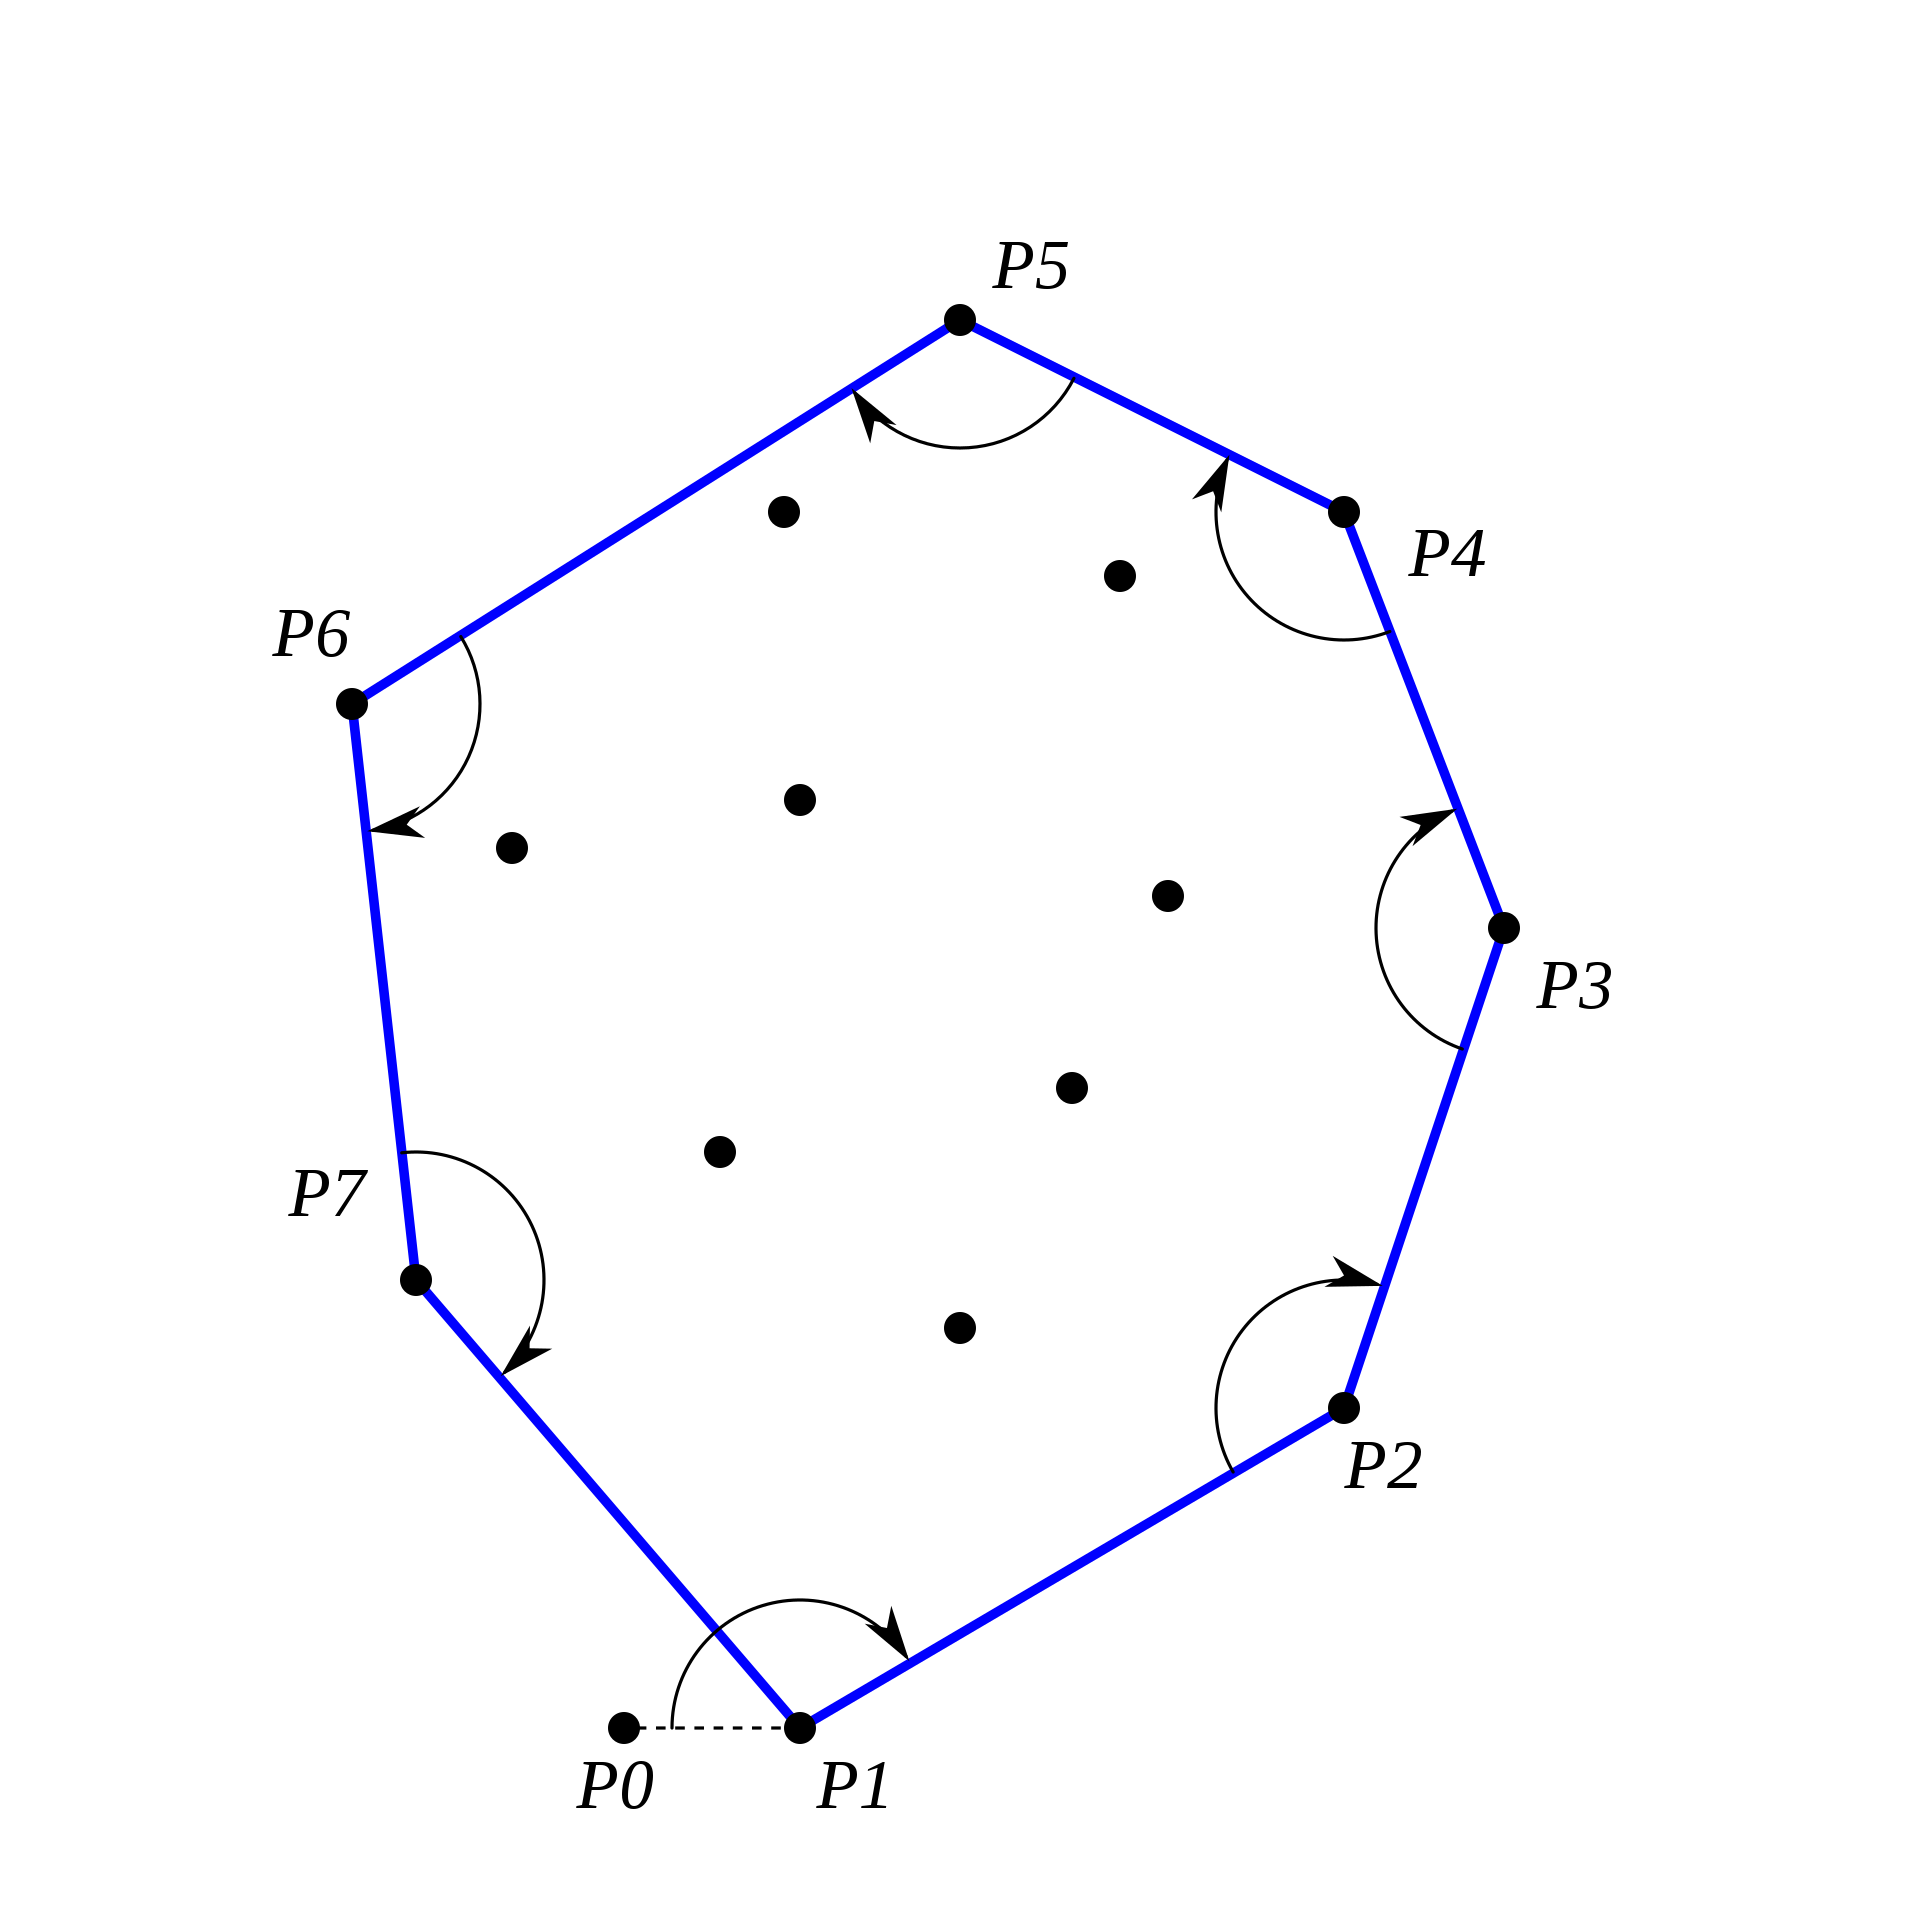
\includegraphics[width=\linewidth]{jarvis.png}

    \subsection{QuickHull}

    https://upload.wikimedia.org/wikipedia/commons/9/9e/Quickhull.gif

    \newpage

    \section{Problemy P, NP, NP-zupełne i zależności między nimi. Hipoteza P vs. NP.}

    \textbf{P vs NP - przykład:}

    \begin{center}
        \textit{Czy jakikolwiek podzbiór zadanego zbioru {-2,6,-3,72,10,-11} sumuje się do zera?}
    \end{center}

    \noindent Trudno znaleźć rozwiązanie tego zagadnienia w czasie wielomianowym. Nasuwający się algorytm sprawdzenia wszystkich
    możliwych podzbiorów ma złożoność wykładniczą ze względu na liczebność zbioru. \textbf{Nie wiadomo zatem czy problem ten
    jest klasy P}.\\

    \noindent Na pewno natomiast uzyskawszy z zewnątrz kandydata na rozwiązanie (np. {-2,6,-3,10,-11}) można w
    liniowym, czyli również wielomianowym, czasie sprawdzić czy sumuje się do zera. \textbf{Jest to zatem problem NP}.


    \newpage

    \section{Automat minimalny, wybrany algorytm minimalizacji.}
    \subsection{Automat minimalny}
    Konstrukcja automatu minimalnego oparta na pochodnych brzozowskiego opisana została w sekcji \textbf{32.1}

    \subsection{Minimalizacja automatu}
    \begin{exercise}
        Niech A = \{a, b\} będzie alfabetem. \\
        Zminimalizuj automat $\mathcal{A} = (S, A, f, s_0, T)$, gdzie S = \{0, 1, 2, 3, 4, 5, 6\}, \\
        $s_0$ = 0, T = \{2, 3, 4, 5, 6\}, a f to funkcja przejść zdefiniowana w tabeli poniżej
    \end{exercise}

    \begin{table}[H]
        \centering
        \begin{tabular}{|c|c|c|c|c|c|c|c|}
            \hline
            f & 0 & 1 & 2 & 3 & 4 & 5 & 6 \\ \hline
            a & 1 & 1 & 2 & 1 & 6 & 5 & 6 \\ \hline
            b & 2 & 3 & 4 & 5 & 2 & 3 & 6 \\ \hline
        \end{tabular}
    \end{table}

    \noindent Zgodnie z algorytmem rozpoczynamy od dwóch zbiorów: stanów terminalnych i pozostałych:
    \begin{verbatim}
        I II
        {0, 1}, {2, 3, 4, 5, 6}
    \end{verbatim}

    \noindent Zbiory są ponumerowane. W następnych krokach będziemy sprawdzać do jakich zbiorów będziemy trafiać zaczynając od danego stanu pod wpływem wszystkich liter alfabetu,
    a następnie rozdzielać te zbiory na tej podstawie:
    \begin{verbatim}
        I II
        { 0 , 1  }, { 2 , 3 , 4 , 5 , 6  }
        I,II I,II II I,II II II II
    \end{verbatim}

    \noindent Jak widać na powyższym przykładzie ze stanu 0 pod wpływem litery a przechodzimy do stanu 1, który jest aktualnie w zbiorze I,
    a pod wpływem litery b przechodzimy do stanu 2, który jest aktualnie w zbiorze II - stąd pod stanem 0 napisaliśmy I,II.
    Dla odmiany ze stanu 2 pod wpływem a przechodzimy do stanu 2, który aktualnie znajduje się w zbiorze II,a pod wpływem b przechodzimy do stanu 4,
    który aktualnie również znajduje się w zbiorze II, stąd pod stanem 2 mamy napisane tylko II. \\

    \noindent Jak widzimy wszystkie stany ze zbioru I trafiają do tych samych ''grup" zbiorów - wszystkie trafiają do I,II (kolejność nie ma znaczenia),
    więc zbiór I nie wymaga na razie podziału. W przypadku zbioru II, stan 3 trafia do innego zestawu zbiorów niż pozostałe stany, więc musimy go wydzielić ze zbioru:
    \begin{verbatim}
        I II III
        {0, 1}, {3}, {2, 4, 5, 6}
    \end{verbatim}

    \noindent Całą procedurę powtarzamy, aż do ustabilizowania się zbiorów (braku nowych podziałów): \\
    \noindent Wyliczenia dla 3 możemy pominąć - zbioru 1-elementowego już nie podzielimy
    \begin{verbatim}
        I II III
        {  0 , 1  }, {  3  }, {  2 , 4 , 5 , 6  }
        I,III I,II III III II,III III

        I II III IV V
        {0}, {1}, {3}, {5}, {  2 , 4 , 6  }
        V V V

        I II III IV V
        {0}, {1}, {3}, {5}, {2, 4, 6}
    \end{verbatim}

    \noindent Jak widzimy zbiory się ustabilizowały. Te zbiory reprezentują stany naszego automatu minimalnego.
    Stanem początkowym jest ten zbiór, w którym znajduje się stan początkowy oryginalnego automatu.
    Stanami końcowymi są te zbiory, w których znajduje się przynajmniej jeden stan końcowy oryginalnego automatu. \\

    \noindent Nasz zminimalizowany automat wygląda następująco:
    \begin{center}
        \begin{tikzpicture}[scale=0.2]
            \tikzstyle{every node}+=[inner sep=0pt]
            \draw [black] (22.4,-32.1) circle (3);
            \draw (22.4,-32.1) node {$I$};
            \draw [black] (38.7,-39.6) circle (3);
            \draw (38.7,-39.6) node {$II$};
            \draw [black] (51.9,-23) circle (3);
            \draw (51.9,-23) node {$III$};
            \draw [black] (51.9,-23) circle (2.4);
            \draw [black] (38.7,-15.6) circle (3);
            \draw (38.7,-15.6) node {$IV$};
            \draw [black] (38.7,-15.6) circle (2.4);
            \draw [black] (25.4,-18) circle (3);
            \draw (25.4,-18) node {$V$};
            \draw [black] (25.4,-18) circle (2.4);
            \draw [black] (23.02,-29.17) -- (24.78,-20.93);
            \fill [black] (24.78,-20.93) -- (24.12,-21.61) -- (25.1,-21.82);
            \draw (24.64,-25.4) node [right] {$b$};
            \draw [black] (41.481,-40.693) arc (96.27369:-191.72631:2.25);
            \draw (44.2,-45.08) node [below] {$a$};
            \fill [black] (39.52,-42.47) -- (39.11,-43.32) -- (40.11,-43.21);
            \draw [black] (39.115,-36.632) arc (167.37011:115.6478:18.394);
            \fill [black] (49.1,-24.07) -- (48.16,-23.97) -- (48.6,-24.87);
            \draw (42.1,-27.79) node [left] {$b$};
            \draw [black] (37.377,-12.92) arc (234:-54:2.25);
            \draw (38.7,-8.35) node [above] {$a$};
            \fill [black] (40.02,-12.92) -- (40.9,-12.57) -- (40.09,-11.98);
            \draw [black] (51.146,-25.901) arc (-18.33446:-58.64763:22.821);
            \fill [black] (41.36,-38.21) -- (42.3,-38.22) -- (41.78,-37.37);
            \draw (47.91,-34.35) node [right] {$a$};
            \draw [black] (24.704,-15.094) arc (221.19573:-66.80427:2.25);
            \draw (28.16,-10.76) node [above] {$a,\mbox{ }b$};
            \fill [black] (27.28,-15.68) -- (28.21,-15.53) -- (27.56,-14.78);
            \draw [black] (41.69,-15.488) arc (85.07615:36.37334:12.157);
            \fill [black] (50.44,-20.39) -- (50.36,-19.45) -- (49.56,-20.04);
            \draw (47.59,-16.49) node [above] {$b$};
            \draw [black] (25.13,-33.35) -- (35.97,-38.35);
            \fill [black] (35.97,-38.35) -- (35.46,-37.56) -- (35.04,-38.47);
            \draw (29.62,-36.36) node [below] {$a$};
            \draw [black] (48.917,-22.732) arc (-100.78239:-137.76812:15.237);
            \fill [black] (40.49,-18) -- (40.65,-18.93) -- (41.39,-18.26);
            \draw (43.32,-21.56) node [below] {$b$};
        \end{tikzpicture}
    \end{center}

    \newpage

    \section{Lemat o pompowaniu dla języków regularnych.}
    \begin{exercise}
        Wykorzystując lemat o pompowaniu udowodnij, że język $\{a^n b^m c^{n+m} | n, m > 0\} \subset \{a, b, c\}^*$ nie jest regularny
    \end{exercise}

    \noindent Załóżmy, że język ten jest regularny. Wtedy zgodnie z lematem o pompowaniu:
    \begin{center}
        $\exists N \in \mathbb{N}_1 : \forall w \in L : |w| \geq N$ $\exists v_1, v_2 \in A^*$ $\exists u \in A^+$ $|v_1 u| < N$ \\
        $w = v_1 u v_2$   $v_1 u^* v_2 \subset L$ \\
        $\forall_i \geq 0$    $v_1 u^i v_2 \in L$
    \end{center}

    \noindent Niech nasze $w = a^N b^N c^{2N}$. Rozważmy wszystkie możliwe podziały słowa w, takie że $|v_1 u| < N$. W przypadku tak dobranego słowa jest tylko jeden typ takiego podziału: \\
    \noindent $v_1 = a^{N-i}$ \\
    \noindent $u = a^i$ \\
    \noindent gdzie $1 \leq i \leq N-1$ \\

    \noindent Musimy teraz znaleźć takie j dla którego słowo $v_1 u^j v_2 \notin L$. Takie j to np. 2 (choć tutaj zasadniczo każde $j \neq 1$ się nadaje).
    Dla j = 2 nasze słowo przyjmuje postać $a^{N+i} b^N c^{2N} \notin L$, więc ten język nie jest językiem regularnym.

    \newpage
    \section{Warunki równoważne definicji języka regularnego: automat, prawa kongruencja syntaktyczna, wyrażenia regularne.}

    \begin{exercise}
        Dla automatu $\mathcal{A}$ zdefiniuj prawą kongruencję syntaktyczną
        oraz wyrażenie regularne opisujące język L akceptowany przez automat $\mathcal{A}$.

        \begin{center}
            \begin{tikzpicture}[scale=0.2]
                \tikzstyle{every node}+=[inner sep=0pt]
                \draw [black] (21.7,-16.4) circle (3);
                \draw (21.7,-16.4) node {$s_0$};
                \draw [black] (34,-16.4) circle (3);
                \draw (34,-16.4) node {$s_1$};
                \draw [black] (45.4,-16.4) circle (3);
                \draw (45.4,-16.4) node {$s_2$};
                \draw [black] (45.4,-16.4) circle (2.4);
                \draw [black] (19.02,-17.723) arc (-36:-324:2.25);
                \draw (14.45,-16.4) node [left] {$b$};
                \fill [black] (19.02,-15.08) -- (18.67,-14.2) -- (18.08,-15.01);
                \draw [black] (22.883,-13.675) arc (142.76071:37.23929:6.239);
                \fill [black] (32.82,-13.67) -- (32.73,-12.74) -- (31.93,-13.34);
                \draw (27.85,-10.71) node [above] {$a$};
                \draw [black] (32.724,-19.083) arc (-39.11992:-140.88008:6.282);
                \fill [black] (22.98,-19.08) -- (23.09,-20.02) -- (23.87,-19.39);
                \draw (27.85,-21.9) node [below] {$b$};
                \draw [black] (37,-16.4) -- (42.4,-16.4);
                \fill [black] (42.4,-16.4) -- (41.6,-15.9) -- (41.6,-16.9);
                \draw (39.7,-16.9) node [below] {$a$};
                \draw [black] (48.08,-15.077) arc (144:-144:2.25);
                \draw (52.65,-16.4) node [right] {$a,b$};
                \fill [black] (48.08,-17.72) -- (48.43,-18.6) -- (49.02,-17.79);
            \end{tikzpicture}
        \end{center}
    \end{exercise}

    \noindent $[1] = (b + ab)^*$ \\
    \noindent $[a] = (b + ab)^*a$ \\
    \noindent $[a^2] = (b + ab)^*a^2(a+b)^*$ \\
    \noindent $\alpha = (b + ab)^*a^2(a+b)^*$

    \newpage
    \section{Automaty niedeterministyczne i deterministyczne (w tym ze stosem); determinizacja.}
    \subsection{Determinizacja automatu niedeterministycznego}
    $\mathcal{A}_{ND}:$

    \begin{center}
        \begin{tikzpicture}[scale=0.2]
            \tikzstyle{every node}+=[inner sep=0pt]
            \draw [black] (11.9,-15.1) circle (3);
            \draw (11.9,-15.1) node {$s_0$};
            \draw [black] (22.8,-8.6) circle (3);
            \draw (22.8,-8.6) node {$s_1$};
            \draw [black] (22.8,-22.3) circle (3);
            \draw (22.8,-22.3) node {$s_2$};
            \draw [black] (35,-15.1) circle (3);
            \draw (35,-15.1) node {$s_3$};
            \draw [black] (35,-15.1) circle (2.4);
            \draw [black] (14.48,-13.56) -- (20.22,-10.14);
            \fill [black] (20.22,-10.14) -- (19.28,-10.12) -- (19.79,-10.98);
            \draw (16.41,-11.35) node [above] {$a$};
            \draw [black] (14.4,-16.75) -- (20.3,-20.65);
            \fill [black] (20.3,-20.65) -- (19.9,-19.79) -- (19.35,-20.62);
            \draw (16.4,-19.2) node [below] {$a$};
            \draw [black] (25.38,-20.78) -- (32.42,-16.62);
            \fill [black] (32.42,-16.62) -- (31.47,-16.6) -- (31.98,-17.46);
            \draw (29.84,-19.2) node [below] {$a$};
            \draw [black] (25.45,-10.01) -- (32.35,-13.69);
            \fill [black] (32.35,-13.69) -- (31.88,-12.87) -- (31.41,-13.75);
            \draw (27.9,-12.35) node [below] {$b$};
            \draw [black] (37.68,-13.777) arc (144:-144:2.25);
            \draw (42.25,-15.1) node [right] {$a,b$};
            \fill [black] (37.68,-16.42) -- (38.03,-17.3) -- (38.62,-16.49);
        \end{tikzpicture}
    \end{center}

    Determinizacja $\mathcal{A}_{ND}$, krok po kroku:
    \begin{center}
        \begin{tikzpicture}[scale=0.2]
            \tikzstyle{every node}+=[inner sep=0pt]
            \draw [black] (14.9,-13.3) circle (3);
            \draw (14.9,-13.3) node {$\{s_0\}$};
        \end{tikzpicture}
    \end{center}

    \begin{center}
        \begin{tikzpicture}[scale=0.2]
            \tikzstyle{every node}+=[inner sep=0pt]
            \draw [black] (14.9,-13.3) circle (3);
            \draw (14.9,-13.3) node {$\{s_0\}$};
            \draw [black] (25.6,-13.3) circle (4);
            \draw (25.6,-13.3) node {$\{s_1,\mbox{ }s_2\}$};
            \draw [black] (17.9,-13.3) -- (20.6,-13.3);
            \fill [black] (21.6,-13.3) -- (20.8,-12.8) -- (20.8,-13.8);
            \draw (19.75,-13.8) node [below] {$a$};
        \end{tikzpicture}
    \end{center}

    \begin{center}
        \begin{tikzpicture}[scale=0.2]
            \tikzstyle{every node}+=[inner sep=0pt]
            \draw [black] (14.9,-13.3) circle (3);
            \draw (14.9,-13.3) node {$\{s_0\}$};
            \draw [black] (25.6,-13.3) circle (4);
            \draw (25.6,-13.3) node {$\{s_1,\mbox{ }s_2\}$};
            \draw [black] (37.6,-13.3) circle (3);
            \draw (37.6,-13.3) node {$\{s_3\}$};
            \draw [black] (37.6,-13.3) circle (2.4);
            \draw [black] (17.9,-13.3) -- (20.6,-13.3);
            \fill [black] (21.6,-13.3) -- (20.8,-12.8) -- (20.8,-13.8);
            \draw (19.75,-13.8) node [below] {$a$};
            \draw [black] (29.6,-13.3) -- (34.6,-13.3);
            \fill [black] (34.6,-13.3) -- (33.8,-12.8) -- (33.8,-13.8);
            \draw (31.6,-13.8) node [below] {$a,b$};
            \draw [black] (39.479,-10.976) arc (168.77514:-119.22486:2.25);
            \draw (44.45,-9.44) node [right] {$a,b$};
            \fill [black] (40.59,-13.38) -- (41.27,-14.02) -- (41.47,-13.04);
        \end{tikzpicture}
    \end{center}


    \newpage
    \subsection{Determinizm automatu ze stosem}
    \begin{exercise}
        Określ, czy podane języki są deterministyczne

        \noindent $L_1 = \{w\overleftarrow{w}\ \; | \; w \in \{a, b\}^*\}$ \\
        \noindent $L_2 = \{wc\overleftarrow{w}\ \; | \; w \in \{a, b\}^*\}$

    \end{exercise}

    \begin{itemize}
        \item $L_1$ jest niedeterministyczny. Automat:
        \begin{center}
            \begin{tikzpicture}[scale=0.2]
                \tikzstyle{every node}+=[inner sep=0pt]
                \draw [black] (11.7,-19.9) circle (3);
                \draw (11.7,-19.9) node {$s_0$};
                \draw [black] (45.4,-19.9) circle (3);
                \draw (45.4,-19.9) node {$s_2$};
                \draw [black] (28.9,-19.9) circle (3);
                \draw (28.9,-19.9) node {$s_1$};
                \draw [black] (59.3,-19.9) circle (3);
                \draw (59.3,-19.9) node {$s_3$};
                \draw [black] (59.3,-19.9) circle (2.4);
                \draw [black] (13.745,-17.719) arc (128.65764:51.34236:10.494);
                \fill [black] (26.86,-17.72) -- (26.54,-16.83) -- (25.92,-17.61);
                \draw (20.3,-14.92) node [above] {$z_0\mbox{ }|\mbox{ }z_0 a$};
                \draw (20.3,-16.42) node [below] {a};
                \draw [black] (26.671,-21.895) arc (-55.76684:-124.23316:11.325);
                \fill [black] (26.67,-21.89) -- (25.73,-21.93) -- (26.29,-22.76);
                \draw (20.3,-24.36) node [below] {$z_0\mbox{ }|\mbox{ }z_0 b$};
                \draw (20.3,-22.86) node [above] {b};
                \draw [black] (31.9,-19.9) -- (42.4,-19.9);
                \fill [black] (42.4,-19.9) -- (41.6,-19.4) -- (41.6,-20.4);
                \draw (37.15,-20.4) node [below] {$1$};
                \draw [black] (27.577,-17.22) arc (234:-54:2.25);
                \draw (28.9,-12.65) node [above] {$1\mbox{ }|\mbox{ }a$};
                \draw (28.9,-14.15) node [below] {a};
                \fill [black] (30.22,-17.22) -- (31.1,-16.87) -- (30.29,-16.28);
                \draw [black] (30.223,-22.58) arc (54:-234:2.25);
                \draw (28.9,-27.15) node [below] {$1\mbox{ }|\mbox{ }b$};
                \draw (28.9,-25.65) node [above] {b};
                \fill [black] (27.58,-22.58) -- (26.7,-22.93) -- (27.51,-23.52);
                \draw [black] (48.4,-19.9) -- (56.3,-19.9);
                \fill [black] (56.3,-19.9) -- (55.5,-19.4) -- (55.5,-20.4);
                \draw (52.35,-18.9) node [above] {$z_0 | 1$};
                \draw (52.35,-20.4) node [below] {$1$};
                \draw [black] (44.077,-17.22) arc (234:-54:2.25);
                \draw (45.4,-12.65) node [above] {$a\mbox{ }|\mbox{ }1$};
                \draw (45.4,-14.15) node [below] {a};
                \fill [black] (46.72,-17.22) -- (47.6,-16.87) -- (46.79,-16.28);
                \draw [black] (46.723,-22.58) arc (54:-234:2.25);
                \draw (45.4,-27.15) node [below] {$b\mbox{ }|\mbox{ }1$};
                \draw (45.4,-25.65) node [above] {b};
                \fill [black] (44.08,-22.58) -- (43.2,-22.93) -- (44.01,-23.52);
            \end{tikzpicture}
        \end{center}
        \item $L_2$ jest deterministyczny. Automat:
        \begin{center}
            \begin{tikzpicture}[scale=0.2]
                \tikzstyle{every node}+=[inner sep=0pt]
                \draw [black] (11.7,-19.9) circle (3);
                \draw (11.7,-19.9) node {$s_0$};
                \draw [black] (45.4,-19.9) circle (3);
                \draw (45.4,-19.9) node {$s_2$};
                \draw [black] (28.9,-19.9) circle (3);
                \draw (28.9,-19.9) node {$s_1$};
                \draw [black] (59.3,-19.9) circle (3);
                \draw (59.3,-19.9) node {$s_3$};
                \draw [black] (59.3,-19.9) circle (2.4);
                \draw [black] (13.745,-17.719) arc (128.65764:51.34236:10.494);
                \fill [black] (26.86,-17.72) -- (26.54,-16.83) -- (25.92,-17.61);
                \draw (20.3,-14.92) node [above] {$z_0\mbox{ }|\mbox{ }z_0 a$};
                \draw (20.3,-16.42) node [below] {a};
                \draw [black] (26.671,-21.895) arc (-55.76684:-124.23316:11.325);
                \fill [black] (26.67,-21.89) -- (25.73,-21.93) -- (26.29,-22.76);
                \draw (20.3,-24.36) node [below] {$z_0\mbox{ }|\mbox{ }z_0 b$};
                \draw (20.3,-22.86) node [above] {b};
                \draw [black] (31.9,-19.9) -- (42.4,-19.9);
                \fill [black] (42.4,-19.9) -- (41.6,-19.4) -- (41.6,-20.4);
                \draw (37.15,-20.4) node [below] {$c$};
                \draw [black] (27.577,-17.22) arc (234:-54:2.25);
                \draw (28.9,-12.65) node [above] {$1\mbox{ }|\mbox{ }a$};
                \draw (28.9,-14.15) node [below] {a};
                \fill [black] (30.22,-17.22) -- (31.1,-16.87) -- (30.29,-16.28);
                \draw [black] (30.223,-22.58) arc (54:-234:2.25);
                \draw (28.9,-27.15) node [below] {$1\mbox{ }|\mbox{ }b$};
                \draw (28.9,-25.65) node [above] {b};
                \fill [black] (27.58,-22.58) -- (26.7,-22.93) -- (27.51,-23.52);
                \draw [black] (48.4,-19.9) -- (56.3,-19.9);
                \fill [black] (56.3,-19.9) -- (55.5,-19.4) -- (55.5,-20.4);
                \draw (52.35,-18.9) node [above] {$z_0 | 1$};
                \draw (52.35,-20.4) node [below] {$1$};
                \draw [black] (44.077,-17.22) arc (234:-54:2.25);
                \draw (45.4,-12.65) node [above] {$a\mbox{ }|\mbox{ }1$};
                \draw (45.4,-14.15) node [below] {a};
                \fill [black] (46.72,-17.22) -- (47.6,-16.87) -- (46.79,-16.28);
                \draw [black] (46.723,-22.58) arc (54:-234:2.25);
                \draw (45.4,-27.15) node [below] {$b\mbox{ }|\mbox{ }1$};
                \draw (45.4,-25.65) node [above] {b};
                \fill [black] (44.08,-22.58) -- (43.2,-22.93) -- (44.01,-23.52);
            \end{tikzpicture}
        \end{center}
    \end{itemize}
    \newpage
    \section{Problemy rozstrzygalne i nierozstrzygalne w teorii języków.}

    \newpage

    \section{Klasy języków w hierarchii Chomsky’ego oraz ich zamkniętość ze względu na operacje boolowskie, homomorfizmy, itp.}

    \begin{itemize}
        \item Gramatyka $G_1 = (V_N,V_T,P,v_0)$ w której

        $V_N = \{v_0\}, \;\; V_T = \{a\}, \;\; P = \{ v_0 \rightarrow v_0 a, \; v_0 \rightarrow a \}$

        generuje język

        $L(G_1) = \{ a^n : n = 1,2,\dots \}$

        Gramatyka jest typu (3)

        \item Gramatyka $G_2 = (V_N,V_T,P,v_0)$, w której

        $V_N = \{v_0\}, \;\; V_T = \{a\}, \;\; P = \{ v_0 \rightarrow v_0 v_0, \; v_0 \rightarrow a \}$

        generuje język


        $L(G_2) = \{ a^n : n = 1,2,\dots \}$

        Gramatyka jest typu (2)


        \item Gramatyka $G_3 = (V_N,V_T,P,v_0)$, w której

        $V_N = \{v_0, v_1, v_2 \}, \;\; V_T = \{a,b,c\}$

        $P=\{v_0~\rightarrow~abc, v_0~\rightarrow~a v_1 bc, v_1 b~\rightarrow~b v_1,v_1 c~\rightarrow~v_2 bcc, bv_2~\rightarrow~ v_2 b,  \\ av_2~\rightarrow~aav_1, av_2~\rightarrow~aa\}$

        generuje język

        $L(G_3) = \{ a^n b^n c^n : n = 1,2,\dots \}$.
        Gramatyka jest typu (0)
        \\

        Gramatyki $G_1$ i $G_2$ są równoważne.
    \end{itemize}

    \newpage

\end{document}
